\documentclass[12pt]{ucthesis}

% This needs to be added before hyperref
\usepackage[papersize={8.5in,11in},inner=1.5in,outer=1.25in,top=1.25in,bottom=1.25in]{geometry}

\usepackage{bbm}
\usepackage{fixltx2e}
\usepackage{url}
\usepackage{amsmath, amsthm, amssymb}
\usepackage{mathtools}
\usepackage{color}
\usepackage{xspace}
\usepackage{verbatim}
\usepackage{graphicx}
\usepackage{psfrag}
\usepackage{pbox}
\usepackage{epstopdf}
\usepackage{textcomp} % For copyright symbol
\DeclareGraphicsExtensions{.pdf,.eps,.png,.jpg}
\usepackage[font=singlespacing]{subcaption}
\captionsetup[table]{labelfont=bf,font=singlespacing}
\captionsetup[figure]{labelfont=bf,font=singlespacing}
\captionsetup[subfigure]{labelfont=bf,font=singlespacing}
\usepackage[titletoc,title]{appendix}
\usepackage{tabularx}
\usepackage{rotating}
\usepackage{hyperref} % Turns all internal references into links to pages within the document

\usepackage{lmodern} % Use the Latin Modern font
\usepackage[T1]{fontenc} % Use a modern font encoding

\newtheorem{lemma}{Lemma}
%\pdfminorversion=4
% NOTE: To produce blinded version, replace "0" with "1" below.
\newcommand{\blind}{0}

% DON'T change margins - should be 1 inch all around.
\addtolength{\oddsidemargin}{0in}%
\addtolength{\evensidemargin}{0in}%
\addtolength{\textwidth}{0in}%
\addtolength{\textheight}{0in}%
\addtolength{\topmargin}{0in}%



\newcommand{\hb}{\hat{b}}
\newcommand{\ha}{\hat{a}}
\newcommand{\htheta}{\hat{\theta}}
\newcommand{\halpha}{\hat{\alpha}}
\newcommand{\hmu}{\hat{\mu}}
\newcommand{\hsigma}{\hat{\sigma}}
\newcommand{\hphi}{\hat{\phi}}
\newcommand{\htau}{\hat{\tau}}
\newcommand{\heta}{\hat{\eta}}
\newcommand{\E}[1]{\mbox{E}\left[#1\right]}
\newcommand{\Var}[1]{\mbox{Var}\left[#1\right]}
\newcommand{\Indicator}[1]{\mathbbm{1}_{ \left( #1 \right) } }
\newcommand{\dNormal}[3]{ N\left( #1 \left| #2, #3 \right. \right) }
\newcommand{\Beta}[2]{\mbox{Beta}\left( #1, #2 \right)}
\newcommand{\alphaphi}{\alpha_{\hphi}}
\newcommand{\betaphi}{\beta_{\hphi}}
\newcommand{\expo}[1]{ \exp\left\{ #1 \right\}}
\newcommand{\tauSquareDelta}{\htau^2
  \left(\frac{1-\expo{-2\htheta\Delta}}{2\htheta} \right)}
\newcommand{\mumu}{\mu_{\hmu}}
\newcommand{\sigmamu}{\sigma^2_{\hmu}}
\newcommand{\sigmamuexpr}{\log\left( \frac{\VarX}{\EX^2} + 1 \right)}
\newcommand{\mumuexpr}{\log(\EX) -  \log\left( \frac{\VarX}{\EX^2} + 1 \right) /2 }

\newcommand{\EX}{\mbox{E}\left[ X \right] }
\newcommand{\VarX}{\mbox{Var}\left[ X \right] }
\newcommand{\mueta}{\mu_{\heta} }
\newcommand{\sigmaeta}{\sigma^2_{\heta}}
\newcommand{\sigmaetaexpr}{ \log\left( \frac{\VarX}{\EX^2} + 1 \right) }
\newcommand{\muetaexpr}{ \log(\EX) -  \sigmaetaexpr /2 }

\newcommand{\mualpha}{\mu_{\halpha} }
\newcommand{\sigmaalpha}{\sigma^2_{\halpha}}
\newcommand{\sigmaalphaexpr}{ \log\left( \frac{\VarX}{\EX^2} + 1 \right) }
\newcommand{\mualphaexpr}{ \log(\EX) -  \sigmaalphaexpr /2 }

\newcommand{\mutauexpr}{ \frac{2}{T} \EX }
\newcommand{\sigmatauexpr}{ \frac{4}{T^2} \Var{X}}

\newcommand{\alphatau}{\alpha_{\htau^2}}
\newcommand{\betatau}{\beta_{\htau^2}}

\newcommand{\Gam}[2]{\mbox{Gamma}\left( #1, #2 \right) }
\newcommand{\InvGam}[2]{\mbox{Inv-Gamma}\left( #1, #2 \right) }

\makeatletter % Hack to get setspace working properly
\let\@currsize\normalsize
\makeatother
\usepackage{setspace}% http://ctan.org/pkg/setspace

% Set default spacing to double (yes, it should be 1.6 here...)
\linespread{1.6}



\def\newblock{\hskip .11em plus.33em minus.07em}

\begin{document}

\title{Volatility Estimation Methods for High-Frequency and Bivariate
  Open, Close, High, Low Prices} \author{Georgi Dinolov}
\degreeyear{2019} \degreemonth{March} \degree{DOCTOR OF PHILOSOPHY}
\chair{Abel Rodr\'iguez} \committeememberone{Hongyun Wang}
\committeemembertwo{Raquel Prado}
\committeememberthree{Daniele Venturi}
%\committeememberthree{Professor 4} % Uncomment if you have 4 committee members. Also change the next line to `\numberofmembers{4}`
\numberofmembers{4}
\deanlineone{Lori Kletzer}
\deanlinetwo{Vice Provost and Dean of Graduate Studies}
\deanlinethree{}
\field{Statistics and Applied Mathematics}
\campus{Santa Cruz}

\begin{frontmatter}
\maketitle

\copyrightpage

\tableofcontents

\listoffigures

\listoftables

\begin{abstract}
A clear, concise abstract explaining the why, what, and how of your work.
\end{abstract}

\begin{dedication}
\vspace*{\fill}
\begin{center}
  In loving dedication to my wife, Alison, who makes it all worth it.
\end{center}
\vspace*{\fill}
\end{dedication}

\begin{acknowledgements}
  I want to thank my advisers, Professor Abel Rodr\'iguez and
  Professor Hongyun Wang, for helping and mentoring me through
  completing this work. Thank you both for your unyielding patience
  and never losing faith in me. I have learned tremendously, and I
  cannot have done this without you both guiding me at every step. I
  also want to thank both Professor Raquel Prado and Professor
  Athanasios Kottas for advising me during my first as a statistics
  graduate student at UC Santa Cruz, and Professor Prado in particular
  for serving on my dissertation committee. Finally, I want to thanks
  Professor Daniele Venturi for also serving on my committee and
  providing an invaluable perspective.

  I want to thank my wife, Alison, for always supporting me and
  reminding me of the light at the end of the tunnel. Thank you also
  to the rest of my family for your encouragement and love.
\end{acknowledgements}

\end{frontmatter}

\chapter{Introduction}
\documentclass[10pt]{article}

\usepackage{amsthm}
\usepackage[toc,page]{appendix}
\usepackage{amssymb}
\usepackage{bm}
\usepackage{pslatex,palatino,avant,graphicx,color}
\usepackage{colortbl}
\usepackage{fullpage}
\usepackage{mathtools}
\usepackage{natbib}
\usepackage{amsmath}
\usepackage{caption}
%\usepackage{subfigure}
\usepackage{subcaption}
\usepackage{bm}
\usepackage{wrapfig}
\usepackage{enumerate}
\usepackage{rotating}
\usepackage{multirow}
\usepackage{tabularx}
\usepackage{tikz}
\usepackage{pgfplots}
\usepackage{bbm}
\usepackage[titles,subfigure]{tocloft} % Alter the style of the Table of Contents

\newtheorem{lemma}{Lemma}
%\pdfminorversion=4
% NOTE: To produce blinded version, replace "0" with "1" below.
\newcommand{\blind}{0}

% DON'T change margins - should be 1 inch all around.
\addtolength{\oddsidemargin}{0in}%
\addtolength{\evensidemargin}{0in}%
\addtolength{\textwidth}{0in}%
\addtolength{\textheight}{0in}%
\addtolength{\topmargin}{0in}%


\renewcommand{\cftsecfont}{\rmfamily\mdseries\upshape}
\renewcommand{\cftsecpagefont}{\rmfamily\mdseries\upshape} % No bold!

\newcommand{\indicator}[1]{\mathbbm{1}\left( #1 \right) }
\newcommand{\hb}{\hat{b}}
\newcommand{\ha}{\hat{a}}
\newcommand{\htheta}{\hat{\theta}}
\newcommand{\halpha}{\hat{\alpha}}
\newcommand{\hmu}{\hat{\mu}}
\newcommand{\hsigma}{\hat{\sigma}}
\newcommand{\hphi}{\hat{\phi}}
\newcommand{\htau}{\hat{\tau}}
\newcommand{\heta}{\hat{\eta}}
\newcommand{\E}[1]{\mbox{E}\left[#1\right]}
\newcommand{\Var}[1]{\mbox{Var}\left[#1\right]}
\newcommand{\Indicator}[1]{\mathbbm{1}_{ \left( #1 \right) } }
\newcommand{\dNormal}[3]{ N\left( #1 \left| #2, #3 \right. \right) }
\newcommand{\Beta}[2]{\mbox{Beta}\left( #1, #2 \right)}
\newcommand{\alphaphi}{\alpha_{\hphi}}
\newcommand{\betaphi}{\beta_{\hphi}}
\newcommand{\expo}[1]{ \exp\left\{ #1 \right\}}
\newcommand{\tauSquareDelta}{\htau^2
  \left(\frac{1-\expo{-2\htheta\Delta}}{2\htheta} \right)}
\newcommand{\mumu}{\mu_{\hmu}}
\newcommand{\sigmamu}{\sigma^2_{\hmu}}
\newcommand{\sigmamuexpr}{\log\left( \frac{\VarX}{\EX^2} + 1 \right)}
\newcommand{\mumuexpr}{\log(\EX) -  \log\left( \frac{\VarX}{\EX^2} + 1 \right) /2 }

\newcommand{\EX}{\mbox{E}\left[ X \right] }
\newcommand{\VarX}{\mbox{Var}\left[ X \right] }
\newcommand{\mueta}{\mu_{\heta} }
\newcommand{\sigmaeta}{\sigma^2_{\heta}}
\newcommand{\sigmaetaexpr}{ \log\left( \frac{\VarX}{\EX^2} + 1 \right) }
\newcommand{\muetaexpr}{ \log(\EX) -  \sigmaetaexpr /2 }

\newcommand{\mualpha}{\mu_{\halpha} }
\newcommand{\sigmaalpha}{\sigma^2_{\halpha}}
\newcommand{\sigmaalphaexpr}{ \log\left( \frac{\VarX}{\EX^2} + 1 \right) }
\newcommand{\mualphaexpr}{ \log(\EX) -  \sigmaalphaexpr /2 }

\newcommand{\mutauexpr}{ \frac{2}{T} \EX }
\newcommand{\sigmatauexpr}{ \frac{4}{T^2} \Var{X}}

\newcommand{\alphatau}{\alpha_{\htau^2}}
\newcommand{\betatau}{\beta_{\htau^2}}

\newcommand{\Gam}[2]{\mbox{Gamma}\left( #1, #2 \right) }
\newcommand{\InvGam}[2]{\mbox{Inv-Gamma}\left( #1, #2 \right) }

%%% END Article customizations

%%% The "real" document content comes below...

% \newbox{\LegendeA}
% \savebox{\LegendeA}{
%    (\begin{pspicture}(0,0)(0.6,0)
%    \psline[linewidth=0.04,linecolor=red](0,0.1)(0.6,0.1)
%    \end{pspicture})}
% \newbox{\LegendeB}
%    \savebox{\LegendeB}{
%    (\begin{pspicture}(0,0)(0.6,0)
%    \psline[linestyle=dashed,dash=1pt 2pt,linewidth=0.04,linecolor=blue](0,0.1)(0.6,0.1)
%    \end{pspicture})}

\title{Solution to a Non-Seperable Diffusion Equation on a Regular Domain}
\author{Georgi Dinolov, Abel Rodriguez, Hongyun Wang}
\date{} % Activate to display a given date or no date (if empty),
         % otherwise the current date is printed 

\begin{document}
\def\spacingset#1{\renewcommand{\baselinestretch}%
{#1}\small\normalsize} \spacingset{1}

\bigskip

\vspace{1cm}
\noindent

\spacingset{1.00} % 
\section{Introduction}

We consider two-dimensional correlated Brownian motion with absorbing boundaries:
\begin{align}
  X(t) &= x_0 + \mu_x t + \sigma_x W_x(t) &a_x &< X(t) < b_x   \label{eq:X} \\
  Y(t) &= y_0 + \mu_y t + \sigma_y W_y(t) &a_y &< Y(t) < b_y   \label{eq:Y} 
\end{align}
where $W_i$ are standard Brownian motions with
$\mbox{Cov}(W_1(t), W_2(t)) = \rho t$ for $0 < t' \leq t$. In
particular, we find the joint transition density function for
$(X(t), Y(t))$ under the boundary conditions:
\begin{align}
  \Pr\left(X(t) \in dx, Y(t) \in dy,  \min_{t'}X(t') \geq a_x,
  \max_{t'}X(t')\leq b_x, \min_{t'} Y(t')\geq a_y, \max_{t'} Y(t')\leq b_y|  X(0)=x_0, Y(0)=y_0, \theta \right), \label{eq:CDF}
\end{align}
with $\theta := (\mu_x, \mu_y, \sigma_x, \sigma_y, \rho).$ This
function, which we shorten to $q(x,y,t)$ from now on, is the solution
to the Fokker-Planck equation \citep{oksendal2013stochastic}:
\begin{align}
  \frac{\partial}{\partial t} q(x,y,t') &= -\mu_x \frac{\partial}{\partial x}q(x,y,t')
                                         - \mu_y \frac{\partial}{\partial y}q(x,y,t')
                                         + \frac{1}{2}\sigma_x^2 \frac{\partial^2}{\partial x^2}q(x,y,t')
                                         + \rho\sigma_x\sigma_y \frac{\partial^2}{\partial x \partial y}q(x,y,t')
                                         + \frac{1}{2}\sigma_y^2 \frac{\partial^2}{\partial y^2}q(x,y,t'),
  \label{eq:1} \\
  q(a_x, y,t') &= q(b_x,y,t') = q(x,a_y,t') = q(x,b_y,t') = 0, \label{eq:2} \\
   0 &< t' \leq t. \nonumber
\end{align}
Differentiating $q(x,y,t)$ with respect to the boundaries produces the
transition density of a particle beginning and ending at the points
$(X_1(0), X_2(0))$ and $(X_1(t), X_2(t))$, respectively, while
attaining the minima $a_x/a_y$ and maxima $b_x/b_y$ in each coordinate
direction:
\begin{align*}
  \frac{\partial^4}{\partial a_x \partial b_x \partial a_y \partial
  b_y} q(x,y,t) = 
\end{align*}
\begin{align}
  \Pr\left(X(t) \in dx, Y(t) \in dy, \min_{t'}X(t') = a_x,
  \max_{t'}X(t')=b_x, \min_{t'} Y(t')=a_y, \max_{t'} Y(t')=b_y \left| 0 <
  t' \leq t, X(0)=x_0, Y(0)=y_0, \theta \right.\right). \label{eq:pdf}
\end{align}
The transition density (\ref{eq:CDF}) with less than all four
boundaries has been used in computing first passage times
\citep{kou2016first, sacerdote2016first}, with application to
structural models in credit risk and default correlations
\citep{haworth2008modelling, ching2014correlated}. \cite{he1998double}
use variants of (\ref{eq:pdf}) with respect to some of the boundaries
to price financial derivative instruments whose payoff depends on
\textbf{some} of the observed maxima/minima. \cite{rodriguez2012} use
a full likelihood-based (Bayesian) approach to estimate volatility in
\textit{univariate} financial timeseries where open, closing, highest,
and lowest prices are included. Their work
fits into a body of literature and collection of techniques by
practitioners where the observed range of prices is used to make
similar estimates. In this paper we will provide the efficient
numerical methods necessary to carry out similar inferential
procedures with correlated financial timeseries.

Closed-form solutions to (\ref{eq:1}) - (\ref{eq:2}) are available for
some parameter regimes. When $\rho = 0$, the transition density of the
process is the solution to a well-understood Sturm-Liouville problem
where the eigenfunctions of the differential operator are sine
functions. When $a_1 = -\infty$ and $b_1 = \infty$, the method of
images can be used to enforce the remaining boundaries. For either
$a_1, a_2 = -\infty$ or $b_1, b_2 = \infty$, eigenfunction of the
Fokker-Plank equation can be found in radial coordinates. Both of
these techniques are used and detailed by
\cite{he1998double}. However, to the best of our knowledge, there is
no closed-form solution to the general problem in (\ref{eq:1}) -
(\ref{eq:2}). This also limits the available ways to compute
(\ref{eq:pdf}), with the most straightforward approach being finite
difference with respect to the boundary conditions. This, however,
requires one to solve at least 16 eigenvalue problems to evaluate the
density function for a single observation (see Section
\ref{sec:likelihood-calc}), motivating the need for an efficient
numerical method to solve (\ref{eq:1}) - (\ref{eq:2}).

It is still possible to approach the general problem by proposing a
biorthogonal expansion in time and space
(\cite{risken1989fokker-planck}, sections 6.2), where the
eigenfunctions for the differential operator are approximated as a
sine series satisfying the boundary conditions. However, a drawback of
this out-of-the-box solution is that the system matrix for the
corresponding eigenvalue problem is dense. Additionally, for nonzero
$\rho$, it is necessary to have a large number of basis elements for
an accurate approximation. The denseness and size of the resultant
system matrices makes the eigenvalue expansion a slow, if not
unfeasible, solution. An alternative is to use a finite difference
scheme to directly solve the evolution problem after suitable
transformations. However, both of these methods need a high degree of
numerical resolution to produce practically useful approximations of
the transition density. We conjecture that these inefficiencies come
from either using a \textit{separable} representation for the
differential operator (trigonometric series) or introducing numerical
diffusion (finite difference).

In this paper, we propose a solution to the general problem
(\ref{eq:1}) - (\ref{eq:2}) which is obtained by combining a
small-time analytic solution with a finite-element method. Our method
directly takes into account the correlation parameter present in the
differential operator in order to efficiently represent the analytic
small-time solution and propagate it forward in time. We apply our
computational method to estimate equation parameters with a maximum
likelihood approach in settings where the model assumptions of
constant $(\mu_x, \mu_y, \sigma_x, \sigma_y, \rho)$ and Brownian
motion driving stochastic evolution are appropriate. Section
\ref{sec:approximate-sols} outlines some methods we considered,
including the one we used. Section [] includes our numerical
experiments.


\section{Approximate Numerical Solutions} \label{sec:approximate-sols}
Before considering solutions to the full Fokker-Planck equation
(\ref{eq:1}) - (\ref{eq:2}), we simplify the PDE by proposing a
scaling transformation and an exponential decomposition of the
solution, so that we can construct
\begin{align}
  p(x,y,t) &= \exp(\alpha x + \beta y + \gamma t) q\left( x(b_x - a_x) + a_x, \,\, y(b_y - a_y) + a_y, \,\, t \right), \label{eq:q-to-p}
\end{align}
where


\begin{align*}
  \alpha &= -\frac{\mu_x}{\sigma_x^2} - \frac{\rho}{\sigma_x\sigma_y(1-\rho^2)}\left( -\frac{\mu_y}{\sigma_y^2} + \frac{\mu_x \rho}{\sigma_x \sigma_y} \right), \\
  \beta &= \left( -\frac{\mu_y}{\sigma_y^2} + \frac{\mu_x \rho}{\sigma_x \sigma_y} \right), \\
  \gamma &= \frac{1}{2}\left( \frac{\sigma_x}{(b_x-a_x)} \right)^2 \alpha^2 + \frac{1}{2}\left(\frac{\sigma_y}{(b_y-a_y)}\right)^2 \beta^2 + \alpha\beta.
\end{align*}
This new formula satisfies the simpler diffusion equation:
\begin{equation}
  \frac{\partial}{\partial t} p(x,y,t) = \mathcal{L}p(x,y,t),\quad (x,y) \in (0,1) \times (0,1) := \Omega \label{eq:qq}
\end{equation}
subject to the constraints
\begin{align}
  p(x,y,t) &=0, & \mbox{ for } & (x,y) \in \{ x | x = 0\} \cup \{ y | y = 0\}, \nonumber \\
  p(x,y,0) &= \delta\left( x - \frac{x_0-a_x}{b_x - a_x} \right) \delta\left(y-\frac{y_0 - a_y}{b_y - a_y}\right), \nonumber
\end{align}
where the differential operator $\mathcal{L}$ takes the form
\[
  \mathcal{L} = \frac{1}{2} \tau_x^2 \frac{\partial^2}{\partial x^2}
  + \rho\tau_x\tau_y \frac{\partial^2}{\partial x \partial y} + \frac{1}{2}\tau_y^2 \frac{\partial^2}{\partial y^2},
  % \left(  \right)^2
  %                                                   \frac{\partial^2}{\partial x^2}p(x,y,t) + \rho\left( \frac{\sigma_x}{(b_x-a_x)} \right)\left( \frac{\sigma_y}{(b_y-a_y)} \right)
  %                                                   \frac{\partial^2}{\partial x \partial y}p(x,y,t) +
  %                                        \frac{1}{2}\left( \frac{\sigma_y}{(b_y-a_y)} \right)^2 \frac{\partial^2}{\partial y^2}p(x,y,t) , \label{eq:qq} \\
\]
where $\tau_x = \frac{\sigma_x}{(b_x-a_x)}$,
$\tau_y = \frac{\sigma_y}{(b_y-a_y)}$.  Note here that under this
transformation $\rho$ remains the same as in the original problem. We
will call equation (\ref{eq:qq}) the \textit{normalized} problem and
will consider its solution in terms of the diffusion parameters
$(\tau_x, \tau_y, \rho)$ without a loss of generality.

\subsection{Eigenfunction Expansion} \label{sec:eigenfunction}
Following Section 6.2 of \cite{risken1989fokker-planck}, we may use
the biorthogonal decomposition of the solution as a sum of
eigenfunctions and time-dependent coefficients determined by eigenvalues:
\begin{equation}
  p(x,y,t) = \phi_\nu(x,y) e^{-\lambda_\nu t}, \label{eq:biorthogonal}
\end{equation}
where the eigenfunctions $\phi_\nu(x, y)$ satisfy the boundary
conditions. Because the differential operator $\mathcal{L}$ is
self-adjoint, the family of eigenfunctions is complete in the Hilbert
space $L_2(\Omega)$. Moreover, the eigenvalues are bounded below by a
positive constant $c$, so that the solution behaves as expected (see
section 6.3 of \cite{risken1989fokker-planck}).

Since we require $\phi_\nu(x,y)$ to be zero on the boundaries, we
may represent the eigenfunction as a linear combination of sines
\[
  \phi_\nu(x,y) = \sum_{l=0}^L \sum_{m=0}^M c_{l,m, \nu}
  \sin\left(2\pi\, l\, x \right) \sin\left(2\pi\, m\, y \right) := \Psi(x,y)^T c_\nu,
\]
where we have truncated the infinite series for some suitably large
$L$ and $M$ and defined
\begin{align*}
  \psi_{l,m}(x,y) &= \sin\left(2\pi\, l\, x \right)
                         \sin\left(2\pi\, m\, y \right), \\
  \Psi(x,y) &= (\psi_{0,0}(x,y), \ldots, \psi_{L,M}(x,y))^T, \\
  c_\nu &= (c_{0,0,\nu}, \ldots, c_{L,M,\nu})^T.
\end{align*}

The biorthogonal representation (\ref{eq:biorthogonal}) leads to the
eigenvalue problem
\begin{equation}
  \mathcal{L} \phi_\nu = -\lambda_\nu \phi_\nu, \label{eq:eigenproblem}
\end{equation}
where $\mathcal{L}$ is the differential operator in the normalized
Fokker-Planck equation. Applying $\mathcal{L}$ to $\phi_\nu$ produces
the linear system
\[
  \mathcal{L}\phi_\nu = \mathcal{L}(\Psi(x,y)^T c_\nu) =
  \mathcal{L}(\Psi(x,y)^T) c_\nu = (A \Psi(x,y))^T c_\nu,
\] 
where $A$ is a constant matrix dependent on $\tilde{\theta}$. In the
case where $\rho = 0$, $A$ is diagonal because
$\left\{ \psi_{l,m}(x,y) \right\}_{l,m}$ are the eigenfunctions to
$\mathcal{L}$. When $\rho \neq 0$, $A$ is no longer diagonal and is in
fact dense. This caused by the mixing terms
\[
  \frac{\partial^2}{\partial x \partial y} \sin\left(2\pi\, l\,
    x\right) \sin\left(2\pi\, m\, y\right) = (2\pi\, l)(2\pi\, m)
  \cos\left(2\pi\, l\, x\right) \cos\left(2\pi\, m\, y\right)
\]
being the products of cosine functions, which have an inefficient sine
series representation [CITE]. Substituting the linear representation
of $\mathcal{L}\phi_\nu$ into the eigenvalue problem
(\ref{eq:eigenproblem}), we arrive to the system
\[
  \Psi(x,y)^T A^T c_\nu = -\lambda_\nu \Psi(x,y)^T c_\nu
  \quad \Leftrightarrow \quad A^T c_\nu = -\lambda_\nu c_\nu
\]
whose solution gives the family of orthonormal eigenfunctions. As
mentioned already, the efficiency of this approach is dependent on the
cost of solving the eigenvalue problem
$A^T c_\nu = -\lambda_\nu c_\nu$.

With all of the eigenpairs $(c_\nu, \lambda_\nu)$, the approximate solution is then
\[
  p(x,y,t) \approx \sum_{\nu}\Psi(x,y)^T c_\nu e^{-\lambda_\nu t}.
\]

\subsubsection{Likelihood Calculation} \label{sec:likelihood-calc}
Recalling equation (\ref{eq:pdf}), to compute the likelihood we are
interested in we must take derivatives of the solution $p(x,y,t)$ with
respect to the boundary parameters $(a_x, b_x, a_y, b_y)$. Because the
eigenvalues and eigenvectors for this problem are functions of the
parameters without explicit analytic form,
$\frac{\partial^4}{\partial a_x\partial b_x \partial a_y \partial
  b_y}p(x,y,t)$ must be computed numerically using a finite difference
approximation. We must therefore find the eigenvalues and
eigenvectors for each of the sixteen perturbed problems
\[
  p(x,y,t | a_x \pm \epsilon, b_x \pm \epsilon, a_y \pm \epsilon, b_y \pm \epsilon),
\]
such that
\[
  \frac{\partial^4}{\partial a_x\partial b_x \partial a_y \partial
    b_y}p(x,y,t) \approx \frac{\sum_{k} c_k p(x,y,t | a_x \pm \epsilon, b_x \pm \epsilon, a_y \pm \epsilon, b_y \pm \epsilon)}{(2\epsilon)^4}.
\]
Because a good, working approximation to $p(x,y,t)$ requires many
terms in the expansion of the eigenfunctions, and because each
resultant system matrix is dense, repeated computation of the
likelihood in this way is unfeasible.

\subsection{Finite Difference} \label{sec:finite-difference} A finite
difference method which approximates the spatial derivatives in
problem (\ref{eq:qq}) requires the solution a system of differential
equations
\begin{align}
  \dot{c}(t)= A c(t) &\Rightarrow& c(t) = \exp\left( At \right)c(0) \label{eq:eigenproblem-fd}, 
\end{align}
which reduces to the eigenvalue decomposition of a matrix $A$. Here,
$c(t)$ is a vector of coefficients representing the value of the
solution in (\ref{eq:qq}) on each point on a grid over $\Omega$ at
time $t$, and the product $Ac(t)$ approximates
$\mathcal{L}p(x,y,t)$. The system matrix $A$ is dependent on the
discretization scheme used to approximate $\mathcal{L}$. Using a
central in space scheme over a \textbf{regular} grid on $\Omega$ with
$\Delta x = \Delta y = h$,
\[ A = \frac{1}{2}\tau_x^2 \frac{1}{h^2}A_{x,x} +
  \rho\tau_x\tau_y \frac{1}{4h^2}A_{x,y} + \frac{1}{2}\tau_y^2
  \frac{1}{h^2}A_{y,y},
\]
where each of the matrices $A_{x,x}, A_{x,y}, A_{y,y}$ approximate
$\frac{\partial^2}{\partial x^2}, \frac{\partial^2}{\partial
  x \partial y}, \frac{\partial^2}{\partial y^2}$, respectively. For
example, using the labeling $c_{l,m}(t) \to c_k(t)$ on the vector
$c(t)$ to denote the approximation of the solution at point
$(x_l, y_m)$ on the grid,
\begin{align*}
  \frac{1}{2}\tau_x^2 \frac{\partial^2}{\partial x^2} p(x_l,y_m,t) \approx \frac{1}{2}\tau_x^2 \left( \frac{c_{l+1,m}(t) - 2c_{l,m}(t) + c_{l-1,m}(t)}{h^2} \right) = \frac{1}{2}\tau_x^2 \frac{1}{h^2}A_{x,x}[k,] c(t) 
\end{align*}
where $A_{x,x}[k,]$ is the $k^{th}$ row of $A_{x,x}$. Similarly,
\begin{align*}
  \rho\tau_x\tau_y \frac{\partial^2}{\partial x \partial y} p(x_l,y_m,t) \approx \rho\tau_x\tau_y \left( \frac{c_{l+1,m+1}(t) - c_{l+1,m-1}(t) - c_{l-1,m+1}(t) + c_{l-1,m-1}(t)}{4h^2} \right) = \rho\tau_x\tau_y \frac{1}{4h^2}A_{x,y}[k,] c(t) 
\end{align*}
It should be noted here that a regular grid approach with a constant
$h$ is appealing, because it allows us to construct once and store the
matrices $A_{x,x}, A_{x,y}, A_{y,y}$, which saves valuable
computational resources if we are to solve the finite difference
eigenproblem (\ref{eq:eigenproblem-fd}) repeatedly for different
parameter values $(\tau_x,\tau_y,\rho)$.

Unlike the system matrix for the trigonometric expansion, the system
matrix $A$ here is sparse: each row of $(A_{x,x}, A_{x,y}, A_{y,y})$
is composed of all zeros except for three or four entries. This
structure does not change as $h \to 0$. The eigenvalue problem is
therefore much cheaper to solve. The system matrix can be made even
sparser on a regular grid by performing a $45^{\circ}$ rotation which
removes the mixing term
$\rho\tau_x \tau_y\frac{\partial^2}{\partial x \partial y}$ from
the problem PDE and preserves the boundaries.

However, the fundamental limitation of using a finite difference
method is that differentiation with respect to boundaries is also done
using finite differences and it is of fourth order. Given this high
order differentiation, $h$ cannot be made too small because truncation
error becomes an issue relatively quickly. More explicitly, assuming
consistency and stability of the finite difference approximation to
$\mathcal{L}$, we can write down the finite difference solution as
\[
  p_{FD}(x_l,y_m,t | a_x) = p(x_l,y_m,t) + O(h^2; a_x).
\]
Note here the residual term $O(h^2; a_x)$ a function of the paramter
$a_x$. The finite difference approximation yields:
\begin{align*}
  \frac{p_{FD}(x_l,y_m,t | a_x) - p_{FD}(x_l,y_m,t | a_x - \epsilon)}{\epsilon} &= \frac{p(x_l,y_m,t | a_x) - p(x_l,y_m,t | a_x - \epsilon)}{\epsilon} + \frac{O(h^2 | a_x) - O(h^2 | a_x - \epsilon)}{\epsilon} \\
      &\approx \frac{\partial}{\partial a_x} p(x_l,y_m,t) + O(\epsilon) + \frac{O(h^2 | a_x) - O(h^2 | a_x - \epsilon)}{\epsilon}.
\end{align*}
If the residual term $O(h^2 | a_x)$ is differentiable with respect to
$a_x$,
\[
  \frac{O(h^2 | a_x) - O(h^2 | a_x - \epsilon)}{\epsilon} \to O(h^2) \mbox{ as } \epsilon \to 0.
\]
Otherwise
\[
  \frac{O(h^2 | a_x) - O(h^2 | a_x - \epsilon)}{\epsilon} \to O(h^2/\epsilon^r) \mbox{ as } \epsilon \to 0.
\]
for some $r > 0$. Under this condition, as $\epsilon \to 0$ with $h$
fixed, the term $O(h^2/\epsilon^r)$ begins to dominate the
approximation. Hence, for a fixed $h$, we have a bound on how
accurately we may represent the likelihood function provided the
finite difference residual term is not differentiable with respect to
the boundary parameters.

The finite value for $h$ introduces yet another practical concern. On
a regular grid, the delta function initial condition needs to be
either rounded to the nearest grid point or represented as a weighted
sum of delta functions on the four nearest grid points. Either
approach introduces a numerical diffusion into the problem which, for
a finite $h$, can bias the numerical solution. We will demonstrate
this phenomenon in Section [].

\subsection{Semidiscrete Galerkin Method} \label{sec:semidiscrete-galerkin}
We propose a semidiscrete Galerkin (continuous in time, discrete in
space) solution to the general diffusion problem (\ref{eq:qq}). The
success of this approach is based on an analytic approximation for the
solution $p(x,y,t)$ for small time $t$ and a basic convergence
estimate from approximation theory for semidiscrete Galerkin-type
solutions to parabolic problems. 

Our numerical method produces a functional representation for the
approximate solution which $1)$ imposes a computational burden
comparable to or better than that of the finite difference method and
$2)$ is infinitely differentiable with respect to the boundary
parameters, allowing us to perform the crucial numerical
differentiation with respect to these parameters.

As described in Section \ref{sec:eigenfunction}, the solution to the
model problem has the eigenfunction expansion 
\[
  p(x,y,t) = \sum_{\nu=0}^\infty\phi_\nu(x,y) e^{-\lambda_\nu t}.
\]
Proceeding with the standandard Galerkin approach, we propose a
solution $p_{k}(x,y,t)$ of similar form
\[
  p_{k}(x,y,t) = \sum_{i=0}^k c_i(t) \psi_i(x,y),
\]
where the basis functions $\psi_i(x,y)$ satisfy the boundary
conditions. We also require that all first- and second-order
derivatives of $\psi_i(x,y)$ are in $L_2(\Omega)$, i.e.
$\psi_k(x,y) \in W_{2}^{2}(\Omega)$. In other words, we look for a
solution in the span of $S_k = \{\psi_0, \ldots, \psi_k\}$. Since
$p_k$ is an approximation to the solution $p$, it does not follow the
differential equation exactly nor can it represent the initial
condition fully. We capture this by defining residuals
\begin{align*}
  \frac{\partial}{\partial t} p_k(x,y,t) - \mathcal{L}p_k(x,y,t) &:= R_e(k), \\
  p(x,y,0) - p_k(x,y,0) &:= R_0(k).
\end{align*}
There are various conditions that could be imposed on the residual
functions (see Section 2.10.3 of \cite{norrie1973finite} for a
summary). The \textit{orthogonality} condition coincides with the
Galerkin procedure:
\begin{align}
  \displaystyle \int_{\Omega} R_e(k) \psi_i(x,y) dx\,dy &= 0,& \displaystyle \int_{\Omega} R_0(k) \psi_i(x,y) dx\,dy &= 0,& i = 0,\ldots k, \label{eq:orthogonality-conditions}
\end{align}
which is equivalent to the weak formulation of the heat problem
\begin{align*}
  \left( \partial_t p_k(x,y,t), \psi_i \right) &= \left(\mathcal{L}p_k(x,y,t), \psi_i \right), \\
  \left( p_k(x,y,0), \psi_i \right) &= \left(p(x,y,0), \psi_i\right),
\end{align*}
where $(\cdot, \cdot)$ is the usual inner product in
$L_2(\Omega)$. The orthogonality conditions
(\ref{eq:orthogonality-conditions}) lead to the system of equations
\begin{align}
  M \mathbf{\dot{c}}(t) &= S \mathbf{c}(t), \label{eq:orthogonality-conditions-mat-1}\\
  M \mathbf{c}(0) &= \mathbf{p}(0), \label{eq:orthogonality-conditions-mat-2}
\end{align}
where $M$ is the mass matrix, $S$ is the stiffness matrix, and
$\mathbf{p}(0)$ is the vector projection of $p(x,y,0)$ onto the
span of $S_k$ with elements
\begin{align*}
  M_{ij} &= \displaystyle \int_\Omega \psi_i \psi_j dx\,dy, \\
  S_{ij} &= -\frac{1}{2}\tau_x^2 \displaystyle \int_\Omega \left( \frac{\partial}{\partial x} \psi_i(x,y) \right) \left( \frac{\partial}{\partial x} \psi_j(x,y) \right) dx\,dy -\rho\tau_x\tau_y \displaystyle \int_\Omega \left( \frac{\partial}{\partial x} \psi_i(x,y) \right) \left( \frac{\partial}{\partial y} \psi_j(x,y) \right) dx\,dy \\
         &\quad -\frac{1}{2}\tau_y^2 \displaystyle \int_\Omega \left( \frac{\partial}{\partial y} \psi_i(x,y) \right) \left( \frac{\partial}{\partial y} \psi_j(x,y) \right) dx\,dy \\
  \mathbf{p}_i(0) &= \displaystyle \int_\Omega p(x,y,0) \psi_i(x,y) dx\,dy.
\end{align*}
The entries of $S_{ij}$ are computed with integration by parts and
using the boundary conditions. The semidiscrete Galerkin approximation
becomes
\[
  p_k(x,y,t) = \boldsymbol{\psi}(x,y)^T \exp\left( M^{-1}S\, t \right) \mathbf{c}(0),
\]
with $\boldsymbol{\psi}(x,y) = (\psi_0(x,y), \ldots, \psi_k(x,y))^T.$

A bound on the closeness of the approximate solution $p_k(x,y,t)$ to
the strong solution $p(x,y,t)$ is developed in \cite{bramble1977some}
shows that the Galerkin approximation we use converges to the strong
solution, and it motivates the thrust of our numerical
solution. First, we define the \textit{error} term
\[
  e_k(t) = p(x,y,t) - p_k(x,y,t),
\]
as well as the norm
\[
  \| w \|_2 = \sum_{j=0}^\infty \lambda_j^2 (w, \phi_j)
\]
for the eigenpairs $(\lambda_j, \phi_j)$ of the operator
$\mathcal{L}$. As referred in \cite{bramble1977some}, functions
$w \in L_2(\Omega)$ with $\|w\|_2 < \infty$ are also in $W_2^2(\Omega)$. In a
sense, $\| \cdot \|_2$ measures the variation of functions. Functions
having higher-order eigenmodes have a bigger norm, and vice
versa. Finally, if we have the condition (corresponding to equation
2.1 in \cite{bramble1977some})
\begin{align}
  \| p(x,y,0) - p_k(x,y,0) \|_{L_2(\Omega)} &\leq C\, h(k)^2 \| p(x,y,0) \|_2. \label{eq:ic-bound}
\end{align}
as a decreasing function $h(k)$, Theorem 2.1 in \cite{bramble1977some}
applies and we have the error estimate
\begin{align}
  \| e(t) \|_{L_2(\Omega)} \leq C h(k)^2 \| p(x,y,0) \|_{2}. \label{eq:error-est}
\end{align}
We can ensure condition (\ref{eq:ic-bound}) is met if $S_k$ is complete
in $L_2(\Omega)$ as $k$ grows. The other two conditions for Theorem
2.1 to apply are demonstrated by \cite{bramble1977some} for the
Galerkin method. Equation (\ref{eq:error-est}) can be summarized in a
simple way: the error of the method is controlled by how much
variation the initial condition has; the rate of decrease of the error
is controlled by how well the span of $S_k$ represents the initial
condition compared to the variation of the initial condition.

However, the initial condition for (\ref{eq:qq}) requires all in
eigenmodes being included in the representation of the initial
conditions, so that
\[
  \| p(x,y,0) \|_{2} = \left\| \delta\left( x - \frac{x_0 - a_x}{b_x-a_x}
  \right) \delta\left( y - \frac{y_0 - a_y}{b_y-a_y} \right)\right\|_{2} = +\infty.
\]
It is obvious that we cannot apply the error estimates above. However,
evolving the solution forward in time, even for a short period,
diffuses the delta-function IC and attenuates out the highest
frequency modes. Further, because solutions to the diffusion equation
are smooth, $p(x,y,t_\epsilon)$ will give us a smooth initial function
which will make the error bounds admissible.

\subsubsection{Small-time Solution}
The small-time solution is derived by considering the fundamental
solution $G(x,y,t)$ for the unbounded problem in (\ref{eq:qq}), which
is the bivariate Gaussian density with mean and covariance determined
by the initial condition and the diffusion parameters
\citep{stakgold2011green}. We can then find a small enough
$t_\epsilon$ such that
$G\left(x,y, t_\epsilon \left| \frac{x_0-a_x}{b_x - a_x},
    \frac{y_0-a_y}{b_y - a_y} \right.\right)$ is numerically zero on
the boundaries of $\Omega$. This is done in the following way.
\begin{enumerate}[1.]
\item Scale and rotate the coordinate axes by
  \[
    \left( \begin{array}{c}
             \xi \\
             \eta
           \end{array} \right) = \mbox{Transformation goes here}
             \left( \begin{array}{cc}
             x \\
             y
           \end{array} \right) 
       \]
       so that the problem obeys the diffusion equation. The
       computational domain is transformed to the parallelogram
       $\tilde{\Omega}$. The transformed initial condition will be
       denoted as $(\xi_0, \eta_0)$.

     \item The fundamental solution $G(\xi,\eta,t | \xi_0, \eta_0)$ in
       this coordinate frame which does not take into account
       boundaries follows the bivariate Gaussian probability density
       function
  \[
    G(\xi,\eta,t | \xi_0, \eta_0) = \frac{1}{2\pi t} \exp\left(-\frac{(\xi-\xi_0)^2 +
        (\eta-\eta_0)^2}{2\,t} \right).
  \]
  We define \textbf{distance} between $G(\xi,\eta,t | \xi_0, \eta_0)$
  and any of the linear boundaries of $\tilde{\Omega}$ as the
  Euclidean norm of the segment of the vector extending from
  $(\xi_0,\eta_0)$ and normal to the boundary. There are four such
  distances $d_1, d_2, d_3, d_4$. Assume that they are listed in
  increasing magnitude.

  Setting $t_\epsilon = d_2/8$ ensures that the fundamental solution
  $G(\xi,\eta,t_\epsilon | \xi_0, \eta_0)$ is \textit{at most}
  $\approx 10^{-15}$ on the second-farthest boundary, as well as the
  other two farthest boundaries. In this way,
  $G(\xi,\eta,t_\epsilon | xi_0, \eta_0)$ satisfies the boundary
  condition on the three farthest boundaries numerically.

\item Reflect the point $(\xi_0, \eta_0) \to (\xi_0', \eta_0')$ about
  the closest boundary. The image function
  $G(\xi,\eta,t_\epsilon | \xi_0', \eta_0')$ satisfies the diffusion
  equation and is equal to $G(\xi,\eta,t_\epsilon | \xi_0, \eta_0)$ on
  the closest boundary. Further,
  $G(\xi,\eta,t_\epsilon | \xi_0', \eta_0')$ takes on values less than
  $10^{-15}$ on all other boundaries, because it is outside of
  $\bar{\Omega}$.

  Considering the difference of the two images, the small-time solution 
  \[
    p(\xi,\eta,t_\epsilon) := G(\xi,\eta,t_\epsilon | \xi_0, \eta_0) -
    G(\xi,\eta,t_\epsilon | \xi_0', \eta_0')
  \]
  satisfies all of the boundaries numerically and also satisfies the
  governing diffusion equation. Performing a change of variables
  produces the small-time solution $p(x,y,t_\epsilon)$.
\end{enumerate}
Using Theorem 5.E of \cite{zeidler1995applied}, we can solve for
$p(x,y,t)$ by considering the smooth $p(x,y,t_\epsilon)$ as an initial
condition and evolving it forward in time by $t-t_\epsilon$. The
bigger $t_\epsilon$, the less eigenmodes present in
$p(x,y,t_\epsilon)$, and the more accurate our weak solution according
to the error estimate
\[
  \| e(t) \|_{L_2(\Omega)} \leq C h(k)^2 \| p(x,y,t_\epsilon) \|_{2}.
\]

\subsubsection{Orthonormal Basis Family}
An upper bound of the rate at which the Galerkin approximation
converges to $p(x,y,t)$ is given by condition (\ref{eq:ic-bound}),
namely by how well the initial condition may be approximated via a
projection onto $S_k$. We motivate the construction of the orthonormal
basis functions by once again considering the fundamental solution for
the unbounded problem (\ref{eq:qq}). In the absence of boundaries,
(\ref{eq:qq}) is solved by the function
\[
  G(x,y,t | x_0', y_0') = \frac{1}{2\pi\,\,t\,\, \tau_x\tau_y\sqrt{1-\rho^2}} \exp\left\{ -\frac{1}{2\,t(1-\rho^2)} \left( \frac{(x - x_0')^2}{\tau_x^2} - 2\rho \frac{(x-x_0')(y-y_0')}{\tau_x\tau_y} + \frac{(y - y_0')^2}{\tau_y^2}\right) \right\},
\]
with
$x_0' = (x_0 - a_x)/(b_x-a_x),\quad y_0' = (y_0 - a_y)/(b_y-a_y)$. We
choose the family of basis functions
$S_k = (\psi_0(x,y), \ldots, \psi_k(x,y))$
\begin{align}
  \psi_i(x,y) &= \frac{1}{2\pi \sigma^2\sqrt{1-\tilde{\rho}^2} } \exp\left\{ -\frac{1}{2(1-\tilde{\rho}^2)\sigma^2} \left( (x - x_i)^2 - 2\tilde{\rho} (x-x_i)(y-y_i) + (y - y_i)^2 \right) \right\} x\left(1-x\right)\, y(1-y)
\end{align}
for some parameters $(\tilde{\rho}, \sigma)$ and a collection of
points $\{ (x_i,y_i) \}_{i=0}^k$ which form a grid over
$\Omega$. Essentially, the collection
$\{ \psi_i(x,y| x_i, y_i, \tilde{\rho}, \sigma) \}_{i=0}^k$ is
composed of fundamental solutions to a heat diffusion problem tuned by
$\sigma$ and $\tilde{\rho}$, tampered such that their support is on
$\Omega$, zero on the boundaries, centered on some grid over $\Omega$,
and still smooth. In this manner, our basis function choice is in
keeping with the golden rule for the rate of convergence: \textbf{The
  smoother the solution to the original problem and the smoother the
  functions in the basis space, the faster the convergence of the
  Ritz-Galerkin method.} (Remark 1(c) in Chapter 2 of
\cite{zeidler1995applied}). Moreover, all of the basis functions are
infinitely differentiable with respect to the boundary and diffusion
parameters, so that
$\frac{\partial^4 p_k(x,y,t)}{\partial a_x \partial b_x \partial
  a_y \partial b_y}$ exists and can be computed numerically using
finite differences.

The other critical advantage of these elements is that they better
resolve the small-time solution $p(x,y,t_\epsilon)$ by taking into
account correlation in the covariance of each kernel.
[\textbf{\color{red} if not prove, demonstrate. I'm running out of
  steam on this.}].

\section{Estimation}
Consider the problem of estimating the parameters
$(\mu_x, \mu_y, \sigma_x, \sigma_y, \rho)$ from an i.i.d. sample
$(Z_1, \ldots, Z_n)$ from the process in (\ref{eq:X}) - (\ref{eq:Y}),
where each $Z_i$ is the vector of random variables
\[
  Z_i = (X_i(t), Y_i(t), A_{x,i}, B_{x,i}, A_{y,i}, B_{y,i}).
\]
We say that $Z_i$ is sampled from the distribution corresponding to
the probability density function (\ref{eq:pdf})
\[
  Z_i \sim F(\theta),
\]
where the distribution $F$ has the usual interpretation
\begin{align*}
  F(z = (x, y, a_x, b_x, a_y, b_y) | \theta) &= \Pr\left(X(t) \leq x,
    Y(t) \leq y, \min_{t' \leq t} X(t') \leq a_x, \max_{t' \leq t}
    X(t') \leq b_x, \min_{t' \leq t} Y(t') \leq a_y, \max_{t' \leq t}
                                               Y(t') \leq b_y\right).
\end{align*}

This estimation problem is of particular importance in quantitative
finance where the model equations (\ref{eq:X}) - (\ref{eq:Y}) (with
various bells and whistles attached) are widely used. However, to the
best of our knowledge, all current \textit{likelihood} methods in the
literature either ignore the observed maximum/minimum information or
use some of it. Likelihood-free approaches, like that of
\cite{rogers1991estimating}, on the other hand suffer from not being
able to be easily integrated into a bigger inferential framework.

Since we do not have a closed-form solution for the likelihood, we
will use an iterative derivative-free maximization algorithm (the
Nelder-Mead method; see \cite{lagarias1998convergence} for review and
convergence properties) which requires repeated evauluation of the
likelihood. For moderate to large samples sizes this is feasible,
because our numerical method is specifically designed for
computational efficiency for repeatedly evaluating the density
function (\ref{eq:pdf}). The maximum likelihood estimator (MLE) for
the true parameters based on $n$ samples, which we call
$\hat{\theta}_n := (\hat{\mu}_x, \hat{\mu}_y, \hat{\sigma}_x,
\hat{\sigma}_y, \hat{\rho})$, is especially useful in practical
settings when it exhibits \textit{consistency}, \textit{i.e.}: the MLE
gets closer to the true parameter vector $\theta$ as more data is
collected and included in the likelihood (assuming the model and its
parameters remain constant during the data collection). More
precise, the estimator $\hat{\theta}_n$ is consistent if
\[
  \Pr( | \hat{\theta}_n - \theta | ) \to 0 \qquad \mbox{as} \qquad n \to \infty.
\]

\subsection{Consistency}
In this section we prove that the MLE based on the Galerkin
approximation $p_k(x,y,t)$ to the governing Fokker-Planck equation
(\ref{eq:1}) is consistent. To do so, we first show that the
distribution on $Z$ based on the approximate $p_k(x,y,t)$ converges to
the true distribution $F(\cdot | \theta)$.

Define the function $F_{k(m)}(z | \theta)$
\begin{align}
  F_{k(m; z)}(z | \theta) &= \displaystyle \int_{-\infty}^x \displaystyle \int_{-\infty}^y \displaystyle \int_{-m}^{a_x} \displaystyle \int_{-m}^{a_y} \displaystyle \int_{-\infty}^{b_x} \displaystyle \int_{-\infty}^{b_y} \frac{\partial^4}{\partial a'_x \partial b'_x \partial a'_y \partial b'_y} q_{k(m; z)}(x', y', t)\,\,\, dx'\, dy'\, da'_x\, db'_x\, da'_y\, db'_y, \label{eq:approx-measure} \\
  &:= \Pr_{k} \left(X(t) \leq x,
    Y(t) \leq y, \min_{t' \leq t} X(t') \leq a_x, \max_{t' \leq t}
    X(t') \leq b_x, \min_{t' \leq t} Y(t') \leq a_y, \max_{t' \leq t}
                                               Y(t') \leq b_y\right) \label{eq:approx-meausre-2}
\end{align}
where $q_k$ is the approximation to $q$ based on the $p_k$ (see
equation (\ref{eq:q-to-p})), and $k(m; z)$ is an increasing function of
$m$ that we will define. We will show that the distribution-like
function $F_{k(m; z)}(\cdot |\theta)$ based on the approximation
$\partial^4 q_{k(m; z)}(x,y,t)/(\partial a_x\,\partial b_x\, \partial
a_y\, \partial b_y)$ approaches the true probability distribution
function $F(\cdot | \theta)$ based on the density
$\partial^4 q(x,y,t)/(\partial a_x\,\partial b_x\, \partial
a_y\, \partial b_y)$ as $k \to \infty$. Note here that in
(\ref{eq:approx-meausre}) - (\ref{eq:approx-meausre-2}) we have
implicitly defined the probability of paths taking on values
below $-m$ to be 0.

A key idea in the proof will be the interpretation of the measure $q(x,y,t)$
\begin{align*}
  q(x,y,t) = \\
  \Pr\left(X(t) \in dx, Y(t) \in dy,  \min_{t'}X(t') \geq a_x,
  \max_{t'}X(t')\leq b_x, \min_{t'} Y(t')\geq a_y, \max_{t'} Y(t')\leq b_y|  X(0)=x_0, Y(0)=y_0, \theta \right) = \\
  \Pr_{W}\left(\left\{ \omega \in \Omega | X_\omega(t) \in dx,\,\, Y_\omega(t) \in dy,\,\,  \forall t' \in [0,t]\,\, a_x \leq X_\omega(t') \leq b_x,\,\, \forall t' \in [0,t] \,\, a_b \leq Y_\omega(t') \leq b_y,\,\, X_\omega(0) = Y_\omega(0) = 0 \right\} \right)
\end{align*}
where $\Pr_{W}$ is the Wiener measure on the samples space of all
realizations (paths) $(X_\omega(t), Y_\omega(t))$ from the stochastic
process (\ref{eq:X}) - (\ref{eq:Y}) defined in the usal way using
Kolmogorov's extension of measure (see \cite{freidlin1985functional},
Section 1.2). Our strategy will be to define a family of sets $\left\{ \tilde{A}_m(z) \right\}_{m=0}^\infty$ for any $z=(x,y,a_x,b_x,a_y,b_y)$ such that
\begin{align*}
  \lim_{m \to \infty} \Pr_W \left(  \tilde{A}_m(z) \right) = 
  \Pr \left( X(t) \leq x,
  Y(t) \leq y, \min_{t' \leq t} X(t') \leq a_x, \max_{t' \leq t}
  X(t') \leq b_x, \min_{t' \leq t} Y(t') \leq a_y, \max_{t' \leq t}
  Y(t') \leq b_y \right) = F(z | \theta)
\end{align*}

\begin{lemma}\label{lem:1}
  For $z = (x,y,a_x,b_x,a_y,b_y)$, 
  \[\lim_{m \to \infty} \displaystyle \int_{-\infty}^x \displaystyle
    \int_{-\infty}^y q(x',y',t, a_x-m, b_x, a_y-m, b_y)\,\, dx'\,dy' -
    \displaystyle \int_{-\infty}^x \displaystyle \int_{-\infty}^y
    q(x',y',t, a_x, b_x, a_y, b_y)\,\, dx'\,dy' = F(z | \theta)\]
\end{lemma}
\begin{proof}
Given some $z = (x,y,a_x,b_x,a_y,b_y)$, define the sets
\begin{align*}
  A_m(z) &= \left\{ \omega \in \Omega | X_\omega(t) \leq x,\,\,
Y_\omega(t) \leq y,\,\, \right. \\ & \forall t' \in [0,t]\,\, a_x-m
\leq X_\omega(t') \leq b_x,\,\, \\ & \forall t' \in [0,t] \,\, a_y -
m\leq Y_\omega(t') \leq b_y,\,\, \\ & \left.X_\omega(0) = Y_\omega(0)
= 0 \right\}, \quad \quad m = 0,1,2,... \\
\end{align*}
Note here that $\Pr_{W}(A_m(z)) = \displaystyle \int_{-\infty}^x \displaystyle \int_{-\infty}^y q(x',y',t, a_x-m, b_x, a_y-m, b_y)\,\, dx'\,dy'$.  Next, we define
\begin{align*}
  \tilde{A}_{m}(z) &= A_m(z) \,\, \bigcap \,\, A_0^C(z) \\
                   &= \left\{ \omega \in \Omega | X_\omega(t) \in dx,\,\, \right.\\
                   & \quad \quad \forall t' \in [0,t]\,\, a_x-m \leq X_\omega(t') \leq b_x,\,\, \\
                   & \quad \quad \forall t' \in [0,t] \,\, a_y - m\leq Y_\omega(t') \leq b_y,\,\, \\
                   & \quad \quad \exists t_{a_x} \in [0,t] \,\, s.t. \,\, X_\omega(t_{a_x}) < a_x \,\, , \exists t_{a_y} \in [0,t] \,\, s.t. \,\, X_\omega(t_{a_y}) < a_y, \\
                   & \quad \quad \left.X_\omega(0) = Y_\omega(0) = 0 \right\}
\end{align*}
It is easy to see that $A_{m}(z) \subset A_{m+1}(z)$ and that
$\tilde{A}_{m}(z) \subset \tilde{A}_{m+1}(z)$. Because of the former
relation,
\[
  \Pr_{W}(\tilde{A}_m(z)) = \Pr_W(A_m(z)) - \Pr_{W}(A_0(z)) = \displaystyle \int_{-\infty}^x \displaystyle \int_{-\infty}^y q(x',y',t, a_x-m, b_x, a_y-m, b_y)\,\, dx'\,dy' - \displaystyle \int_{-\infty}^x \displaystyle \int_{-\infty}^y q(x',y',t, a_x, b_x, a_y, b_y)\,\, dx'\,dy'.
\]
Finally,
\begin{align*}
  \bigcup_{m=0}^\infty \tilde{A}_m(z) &= \left\{ \omega \in \Omega | X_\omega(t) \in dx,\,\, \right.\\
                   & \quad \quad \forall t' \in [0,t]\,\, -\infty \leq X_\omega(t') \leq b_x,\,\, \\
                   & \quad \quad \forall t' \in [0,t] \,\, -\infty \leq Y_\omega(t') \leq b_y,\,\, \\
                   & \quad \quad \exists t_{a_x} \in [0,t] \,\, s.t. \,\, X_\omega(t_{a_x}) < a_x \,\, , \exists t_{a_y} \in [0,t] \,\, s.t. \,\, X_\omega(t_{a_y}) < a_y, \\
                   & \quad \quad \left.X_\omega(0) = Y_\omega(0) = 0 \right\},
\end{align*}
such that for $\omega \in \bigcup_{m=0}^\infty \tilde{A}_m(z)$,
$X_\omega(t) \leq x, Y_\omega(t) \leq y, \min_{t'} X_{\omega}(t') \leq
a_x, \min_{t'} Y_{\omega}(t') \leq a_y, \max_{t'} X_{\omega}(t') \leq
b_x$, $\max_{t'} Y_{\omega}(t') \leq b_y$, and
\[
  \Pr_W\left( \bigcup_{m=0}^\infty \tilde{A}_m(z) \right) = \lim_{M \to \infty} \Pr_W\left( \bigcup_{m=0}^M \tilde{A}_M(z) \right) = F(z |
  \theta).
\]
Since $\tilde{A}_{m}(z) \subset \tilde{A}_{m+1}(z)$,
\[
  \lim_{m\to \infty} \Pr_W(\tilde{A}_m(z)) = \lim_{m \to \infty} \displaystyle \int_{-\infty}^x \displaystyle \int_{-\infty}^y q(x',y',t, a_x-m, b_x, a_y-m, b_y)\,\, dx'\,dy' - \displaystyle \int_{-\infty}^x \displaystyle \int_{-\infty}^y q(x',y',t, a_x, b_x, a_y, b_y)\,\, dx'\,dy'  = F(z | \theta)
\]
\end{proof}
For a shorthand, denote
$
  \mu_k(\tilde{A}_m(z)) = \displaystyle \int_{-\infty}^x \displaystyle \int_{-\infty}^y q_k(x',y',t, a_x-m, b_x, a_y-m, b_y)\,\, dx'\,dy' - \displaystyle \int_{-\infty}^x \displaystyle \int_{-\infty}^y q_k(x',y',t, a_x, b_x, a_y, b_y)\,\, dx'\,dy'.
$

\begin{lemma} \label{lem:weak}
  For a fixed $m$, $\mu_k(\tilde{A}_m(z)) \to \Pr_W(\tilde{A}_m(z))$ as $k\to \infty$.
\end{lemma}
\begin{proof}
  The proof for this lemma follows direcly from the convergence result
  $p_k \to p$ as $k\to \infty$ under the $L_2(\Omega)$ norm from
  Section \ref{sec:semidiscrete-galerkin}.
\end{proof}
With the result from Lemma \ref{lem:weak}, we can now define the
function $k(m; z)$ as
\[
  k(m; z) := \inf_{k'}\left\{ \left| \mu_{k'}(\tilde{A}_m(z)) - \Pr_W(\tilde{A}_m(z)) \right| < 1/2m  \right\}
\]

\begin{lemma}\label{lem:convergence-in-dist}
  For $F_{k(m;z)}$, $F$, and $z$ defined above,
  \[ \lim_{m\to \infty} F_{k(m;z)}(z | \theta) = F(z | \theta). \]
\end{lemma}

\begin{proof}
  For any $\epsilon > 0$, let $M_1 = 2/\epsilon$. By Lemma
  \ref{lem:1}, we can find $M_2$ such that $\forall m > M_2$
  $\left| \Pr_W(\tilde{A}_m(z) - F(z | \theta) \right| <
  \epsilon/2$. Let $M = \max\{M_1, M_2\}$. For any $m > M$,
  \begin{align*}
    \left| F_{k(m)}(z) - F(z) \right | &= \left| \mu_{k(m)}(\tilde{A}_m(z)) - F(z) \right | \\
                                       &\leq \left|  \mu_{k(m)}(\tilde{A}_m(z)) - \Pr_W(\tilde{A}_m(z)) \right| + \left|  \Pr_W(\tilde{A}_m(z)) - F(z | \theta) \right|. \\
                                       &\leq \epsilon/2 + \epsilon/2
  \end{align*}
  The left term bound is defined by $k(m;z)$.
\end{proof}

% \begin{lemma}
%   For a fixed $k$,
%   $\lim_{m\to \infty} \mu_k(\tilde{A}_m(z)) = c \in \mathbb{R},$ i.e.
%   $\left\{ \mu_k(\tilde{A}_m(z))\right\}_{m=0}^\infty$ is a convergent
%   sequence.
% \end{lemma}

% \begin{proof}[Proof idea]
%   Here we will present a formal argument, without giving all of the
%   necessary technical details. As $m \to \infty$, the parameters
%   $\tau_x, \tau_y$ in the normalized problem are $O(1/m)$.  Further,
%   the initial condition coordinates tend to
%   $((1-1/m),(1-1/m))$. Letting $\gamma = 1/m$ for $m >> 1$, the
%   normalized problem becomes
%   \begin{equation*}
%     \frac{\partial}{\partial t} p(x,y,t) = \mathcal{L}p(x,y,t),\quad (x,y) \in = \Omega
% \end{equation*}
% with the initial condition
% \begin{align*}
%   p(x,y,0) &= \delta\left( x - (1-\gamma) \right) \delta\left(y-(1-\gamma)\right),
% \end{align*}
% where the differential operator $\mathcal{L}$ is of order
% \[
%   \mathcal{L} = \frac{1}{2} \gamma^2 \frac{\partial^2}{\partial x^2}
%   + \rho\gamma^2 \frac{\partial^2}{\partial x \partial y} + \frac{1}{2}\gamma^2 \frac{\partial^2}{\partial y^2}.
% \]
% This means that fundamental solution to the unbounded problem above is
% the Gaussian density
% \[
%   G(x,y,t'| \gamma) = \frac{1}{2\pi\,\,t'\,\, \gamma^2\sqrt{1-\rho^2}} \exp\left\{ -\frac{1}{2\, t' \, (1-\rho^2)} \left( \frac{(x - 1 + \gamma)^2}{\gamma^2} - 2\rho \frac{(x-1+\gamma)(y-1+\gamma)}{\gamma^2} + \frac{(y - 1 + \gamma)^2}{\gamma^2}\right) \right\}, t' \in (0,t]
% \]
% We claim that according to our method, we can find a constant $\Gamma$
% such that for $\gamma < \Gamma$, $t_\epsilon > t$ for the small-time
% solution $p(x,y,t_\epsilon)$, which means that $G(x,y,t | \gamma)$
% solves the above problem. This means that, \textbf{for fixed} $k$, the
% Galerkin approximation generated by our method is the projection of
% $p(x,y,t)$ onto the basis family $S_k$ (there is no forward evolution
% of the problem).

% Further, because
% $G(x,y,t | \gamma) \to \delta(x-1+\gamma)\delta(y-1+\gamma)$ weakly as
% $\gamma \to 0$, each of the projections of $G(x,y,t | \gamma)$ onto $S_k$ converge to the basis functions evaluated at $((1-\gamma), (1-\gamma))$:
% \[
%   \displaystyle \int_\Omega G(x,y,t | \gamma) \psi_i(x,y) dx\,dy \to \psi_i(1-\gamma,1-\gamma).
% \]
% Given $S_k$, the above coefficients uniquely define $p_k$
% projection is defined only by $p(x,y,t_\epsilon)$ and $S_k$ only on
% $\mathbf{p}(t_\epsilon)$ (see equation
% (\ref{eq:orthogonality-conditions-mat-2})) become the same. Because
% $k$ is fixed, the mass $M$ stays the same, which means that the
% initial condition vectors in the Galerkin method also converge at
% $\gamma \to 0$. Fu
% \end{proof}

\begin{lemma}
  The maximum likelihood estimator is consistent as $n \to \infty$ and $m \to \infty$:
  \[ \hat{\theta}_{n,k} \to \theta \].
\end{lemma}
\begin{proof}
  \textbf{\color{red} It's a bit sloppy. Also, we do not need
    asymptotic efficiency to prove equation (\ref{eq:var-lim})} By
  Lemma \ref{lem:1}
    \[ X_k \xrightarrow[]{d} X \mbox { as } k \to \infty. \] Next,
    given Theorem 4.1 in \cite{singler2008differentiability}, we know
    that, for each $k$, $q_k$ is analytic in both the diffusion
    parameters and boundary parameters. Hence, the probability density
    function satisfies the criteria A1 - A6 in
    \cite{casella2002statistical} to guarantee that, for data
    $X_{k} \sim F_k(\theta)$,
    \[ \hat{\theta}_{n,k}(X_k) \xrightarrow[]{p} \theta \mbox{ as } n
      \to \infty. \]

    Now we need to show that the same holds for data sampled from $F$
    as $k \to \infty$. To do this, we will use Chebyshev's inequality:
  \[
    \Pr_{X}\left( \left| \hat{\theta}_{n,k}(X) - \theta \right| \geq
      \epsilon \right) \leq \frac{ \mbox{E}_{X}\left[
        (\hat{\theta}_{n,k}(X) - \theta)^2 \right] }{ \epsilon^2 }.
  \]
  By the Maximum theorem [REFERENCE], $\hat{\theta}_{n,k}(x)$ is a continuous
  function with respect to $x$, and further because we have bounded
  $\hat{\theta}$ from below and above,
  \[
    \mbox{E}_{X_k}\left[ (\hat{\theta}_{n,k}(X_k) - \theta)^2 \right]
    \to \mbox{E}_{X}\left[ (\hat{\theta}_{n,k}(X) - \theta)^2 \right]
    \mbox{ as } k \to \infty
  \]
  by the portmanteau lemma. Finally, we can show that
  \begin{equation}
    \mbox{E}_{X_k}\left[ (\hat{\theta}_{n,k}(X_k) - \theta)^2 \right]
    \to 0 \mbox{ as } n \to \infty, \label{eq:var-lim}
  \end{equation}
  since the expected value of the estimator tends to $\theta$ and its
  variance goes to 0 when $n \to \infty$. Therefore, given any
  $\epsilon > 0$ and $\delta > 0$, we can find a sufficiently large
  $n$ and $k$ such that
  \[
    \Pr_{X}\left( \left| \hat{\theta}_{n,k}(X) - \theta \right| \geq
      \epsilon \right) \leq \frac{ \mbox{E}_{X}\left[
        (\hat{\theta}_{n,k}(X) - \theta)^2 \right] }{ \epsilon^2 } < \delta    
  \]
\end{proof}


\bibliographystyle{plainnat}
\bibliography{master-bibliography}
\end{document}


\chapter{High-Frequency Stochastic Volatility}
\input{/home/gdinolov/PDE-solvers/src/SV-with-leverage/paper-revisions-7-11-2016/dissertation-chapter-sv-high-freq.tex}
  
\chapter{Volatility Estimation For Bivariate Assets With OCHL Data: A Galerkin Solution}
\label{ch:galerkin}

\section{Introduction}

We consider two-dimensional correlated Brownian motion with absorbing boundaries:
\begin{align}
  X(t) &= x_0 + \mu_x t + \sigma_x W_x(t) &a_x &\leq X(t) \leq b_x   \label{eq:X} \\
  Y(t) &= y_0 + \mu_y t + \sigma_y W_y(t) &a_y &\leq Y(t) \leq b_y   \label{eq:Y} 
\end{align}
where $W_i$ are standard Brownian motions with
$\mbox{Cov}(W_1(t), W_2(t)) = \rho t$. We find the below probability
for $(X(t), Y(t))$ and the random variables
$M_X(t)=\max_{0\leq s\leq t}X(t),$ $m_X(t)=\min_{0\leq s\leq t}X(t),$
$M_Y(t)=\max_{0\leq s\leq t}Y(t),$ $m_Y(t)=\min_{0\leq s\leq t}Y(t)$
\begin{align}
  \mbox{Pr}\left( \left. \begin{array}{ll}
                           X(t) \leq x_t, & Y(t) \leq y_t, \\
                           M_X(t) \leq b_x, & M_Y(t) \leq b_x, \\
                           m_X(t) \geq a_x, & m_Y(t) \geq a_y,
                         \end{array} \right| X(0) = x_0, Y(0) = y_0, \theta \right)
                                              \label{eq:CDF}
\end{align}
with $\theta := (\mu_x, \mu_y, \sigma_x, \sigma_y, \rho).$ This
probability can be expressed as the integral
\[
  \displaystyle \int_{a_x}^{x_t} \displaystyle \int_{a_y}^{y_t} q(x,y,t) dx\,dy,
\]
where $q(x,y,t)$ is the solution to the Fokker-Planck equation
\cite{oksendal2013stochastic}:
\begin{align}
  \displaystyle \frac{\partial}{\partial t'} q(x,y,t') &= -\mu_x \frac{\partial}{\partial x}q(x,y,t')
                                         - \mu_y \frac{\partial}{\partial y}q(x,y,t')
                                         + \frac{1}{2}\sigma_x^2 \frac{\partial^2}{\partial x^2}q(x,y,t')
                                         + \rho\sigma_x\sigma_y \frac{\partial^2}{\partial x \partial y}q(x,y,t')
                                         + \frac{1}{2}\sigma_y^2 \frac{\partial^2}{\partial y^2}q(x,y,t'),
  \label{eq:1} \\
  q(a_x, y,t') &= q(b_x,y,t') = q(x,a_y,t') = q(x,b_y,t') = 0, \label{eq:2} \\
   0 &< t' \leq t. \nonumber
\end{align}
Differentiating $q(x,y,t)$ with respect to the boundaries produces the
transition density of a particle beginning and ending at the points
$(X(0), Y(0))$ and $(X(t), Y(t))$, respectively, while
attaining the minima $a_x/a_y$ and maxima $b_x/b_y$ in each coordinate
direction. This transition density is equivalent to the joint density
for $(X(t), Y(t), m_X(t), M_X(t), m_Y(t), M_Y(t))| X(0)=x_0, Y(0)=y_0$,
which we denote as $f(x,y,a_x,b_x,a_y,b_y)$:
\begin{align}
  \frac{\partial^4}{\partial a_x \partial b_x \partial a_y \partial b_y} q(x,y,t) = f(x,y,a_x,b_x,a_y,b_y).
  \label{eq:pdf}
\end{align}
Probability functions similar to (\ref{eq:CDF}) with less than all
four boundaries have been used in computing first passage times
\cite{kou2016first, sacerdote2016first}, with application to
structural models in credit risk and default correlations
\cite{haworth2008modelling, ching2014correlated}. \cite{he1998double}
use variants of (\ref{eq:pdf}) with respect to some of the boundaries
to price financial derivative instruments whose payoff depends on
\textit{some} of the observed maxima/minima. \cite{rodriguez2012} use
a full likelihood-based (Bayesian) approach to estimate volatility in
\textit{univariate} financial timeseries where open, closing, highest,
and lowest prices are included. Their work fits into a body of
literature and collection of techniques by practitioners where the
observed range of prices is used to make similar estimates. In this
chapter we will provide an efficient numerical method necessary for
carrying out inferential procedures with correlated financial
timeseries in the bivariate setting.

Closed-form solutions to (\ref{eq:1}) - (\ref{eq:2}) are available for
some parameter regimes. When $\rho = 0$, the transition density of the
process is the solution to a well-understood Sturm-Liouville problem
where the eigenfunctions of the differential operator are sine
functions. When $a_x = -\infty$ and $b_x = \infty$, the method of
images can be used to enforce the remaining boundaries. For either
$a_x, a_y = -\infty$ or $b_x, b_y = \infty$, eigenfunctions of the
Fokker-Plank equation can be found in radial coordinates. Both of
these techniques are used and detailed by
\cite{he1998double}. However, to the best of our knowledge, there is
no closed-form solution to the general problem in (\ref{eq:1}) -
(\ref{eq:2}). This also limits the available ways to compute
(\ref{eq:pdf}), with the most straightforward approach being finite
difference with respect to the boundary conditions. This, however,
requires one to solve Fokker-Planck equation (\ref{eq:1}) - (\ref{eq:2})
accurately for at least 16 slightly different sets of boundaries and
combine the results with numerical differentiation to evaluate the
density function for a just single observation (see Section
\ref{sec:likelihood-calc}), motivating the need for an efficient
numerical method to solve (\ref{eq:1}) - (\ref{eq:2}).

For non-zero correlation, it is still possible to approach the general
problem by proposing a biorthogonal expansion in time and space
(\cite{risken1989fokker-planck}, sections 6.2), where the
eigenfunctions for the differential operator are approximated by the
eigenvectors of a linear system obtained using a truncated expansion
based on a set of separable basis function, each of which is a product
of two sine functions (one in each dimension) satisfying the boundary
conditions. However, a drawback of this out-of-the-box solution is
that the system matrix for the corresponding eigenvalue problem is
dense. Additionally, for nonzero $\rho$, it is necessary to have a
large number of basis elements for an accurate approximation. The
denseness and size of the resultant system makes the
expansion a slow, if not unfeasible, solution. An alternative is to
use a finite difference scheme to directly solve the evolution problem
after suitable transformations. However, both of these methods need a
high degree of numerical resolution to produce practically useful
approximations of the transition density. We conjecture that for the
trigonometric series expansion, inefficiencies arise from using a
separable representation for a differential operator that is
intrinsically correlated in the two dimensions; for the finite
difference approach, the problem is twofold as the method introduces
numerical diffusion in the initial condition and it also uses a
separable approximation for the differential operator.

In the following two chapters we propose robust and efficient
solutions to the problems (\ref{eq:1}) - (\ref{eq:2}) and
(\ref{eq:pdf}) in two distinct parameter regimes. The twofold solution
is obtained by combining a small-time analytic solution with a
Galerkin discretization based on basis functions that are
correlated.

This chapter describes the Galkerin discretization, which directly
takes into account the correlation parameter present in the
differential operator in order to efficiently represent an analytic
small-time solution and propagate it forward in time. We apply our
computational method to estimate equation parameters with a maximum
likelihood approach in settings where the model assumptions of
constant $(\mu_x, \mu_y, \sigma_x, \sigma_y, \rho)$ and Brownian
motion driving stochastic evolution are appropriate. Section
\ref{sec:approximate-sols} outlines some methods we considered for
this problem. Section \ref{sec:semidiscrete-galerkin} describes the
Galerkin method we implemented. Section [] includes our numerical
experiments.


\section{Approximate Numerical Solutions} \label{sec:approximate-sols}
Before considering solutions to the full Fokker-Planck equation
(\ref{eq:1}) - (\ref{eq:2}), we simplify the PDE by proposing a series
of transformations to standardize the problem. The first transformation
\begin{align}
  T_{(1)} : q(x,y,t) &\to p(x,y,t)
\end{align}
scales and decomposes the solution while preserving the initial and
boundary conditions while getting rid of the advection terms in the
differential operator. $T_1$ is defined as
\begin{align}
  T_{(1)}: p(x,y,t) &= \exp(\alpha x + \beta y + \gamma t) q\left( x(b_x - a_x) + a_x, \,\, y(b_y - a_y) + a_y, \,\, t \right), \label{eq:q-to-p}
\end{align}
where


\begin{align*}
  \alpha &= -\frac{\mu_x}{\sigma_x^2} - \frac{\rho}{\sigma_x\sigma_y(1-\rho^2)}\left( -\frac{\mu_y}{\sigma_y^2} + \frac{\mu_x \rho}{\sigma_x \sigma_y} \right), \\
  \beta &= \left( -\frac{\mu_y}{\sigma_y^2} + \frac{\mu_x \rho}{\sigma_x \sigma_y} \right), \\
  \gamma &= \frac{1}{2}\left( \frac{\sigma_x}{(b_x-a_x)} \right)^2 \alpha^2 + \frac{1}{2}\left(\frac{\sigma_y}{(b_y-a_y)}\right)^2 \beta^2 + \alpha\beta.
\end{align*}
This new formula satisfies the \textit{pure diffusion} equation:
\begin{equation}
  \frac{\partial}{\partial t} p(x,y,t) = \mathcal{L}_1 p(x,y,t),\quad (x,y) \in (0,1) \times (0,1) := \Omega_1 \label{eq:qq}
\end{equation}
subject to the constraints
\begin{align}
  p(x,y,t) &=0, & \mbox{ for } & (x,y) \in \{ x | x = 0\} \cup \{ y | y = 0\} \cup \{ x | x = 1\} \cup \{ y | y = 1\}, \nonumber \\
  p(x,y,0) &= \delta\left( x - \frac{x_0-a_x}{b_x - a_x} \right) \delta\left(y-\frac{y_0 - a_y}{b_y - a_y}\right), \nonumber
\end{align}
where the differential operator $\mathcal{L}_1$ takes the form
\[
  \mathcal{L}_1 = \frac{1}{2} \tau_x^2 \frac{\partial^2}{\partial x^2}
  + \rho\tau_x\tau_y \frac{\partial^2}{\partial x \partial y} + \frac{1}{2}\tau_y^2 \frac{\partial^2}{\partial y^2},
  % \left(  \right)^2
  %                                                   \frac{\partial^2}{\partial x^2}p(x,y,t) + \rho\left( \frac{\sigma_x}{(b_x-a_x)} \right)\left( \frac{\sigma_y}{(b_y-a_y)} \right)
  %                                                   \frac{\partial^2}{\partial x \partial y}p(x,y,t) +
  %                                        \frac{1}{2}\left( \frac{\sigma_y}{(b_y-a_y)} \right)^2 \frac{\partial^2}{\partial y^2}p(x,y,t) , \label{eq:qq} \\
\]
with $\tau_x = \frac{\sigma_x}{(b_x-a_x)}$,
$\tau_y = \frac{\sigma_y}{(b_y-a_y)}$.  Note here that under this
transformation $\rho$ remains the same as in the original
problem.

Next, we \textit{normalize} the diffusion equation (\ref{eq:qq}) with the transformation
\begin{align}
  T_{(2)}: p(x,y,t) &\to p(\tilde{x}, \tilde{y}, \tilde{t}),
\end{align}
defined with the coordinate transformation
\begin{align}
  \tilde{x} &= x\cdot \Indicator{ \max\left\{\tau_x^2, \tau_y^2 \right\} = \tau_x^2} + y\cdot \Indicator{ \max\left\{\tau_x^2, \tau_y^2 \right\} = \tau_y^2}, \\
  \tilde{y} &= y\cdot \Indicator{ \max\left\{\tau_x^2, \tau_y^2 \right\} = \tau_x^2} + x\cdot \Indicator{ \max\left\{\tau_x^2, \tau_y^2 \right\} = \tau_y^2}, \\
  \tilde{t} &= t\cdot \max\left\{\tau_x^2, \tau_y^2 \right\}.
\end{align}
The differential problem under $T_{(2)}$ now takes on the
\textit{normalized form} (from hereon referred to as the
\textit{normalized problem}):
\begin{align}
  \frac{\partial}{\partial \tilde{t}} p(\tilde{x},\tilde{y},\tilde{t}) &= \mathcal{L}_2 p(\tilde{x},\tilde{y},\tilde{y}), & (\tilde{x}, \tilde{y}) \in (0,1) \times (0,1) := \Omega_2 \label{eq:qqq} \\
  \mathcal{L}_2 &= \frac{1}{2} \frac{\partial^2}{\partial \tilde{x}^2} + \rho \sigma_{\tilde{y}} \frac{\partial^2}{\partial \tilde{x} \partial \tilde{y}} + \frac{1}{2} \sigma^2_{\tilde{y}} \frac{\partial^2}{\partial \tilde{y}^2},
\end{align}
with
$\sigma_{\tilde{y}} = \min\left\{ \tau_x/\tau_y, \tau_y/\tau_x
\right\}$ subject to the IC/BCs:
\begin{align}
  p(\tilde{x},\tilde{y},\tilde{t}) &=0,  \mbox{ for }  (\tilde{x},\tilde{y}) \in \{ \tilde{x} | \tilde{x} = 0\} \cup \{ \tilde{y} | \tilde{y} = 0\} \cup \{ \tilde{x} | \tilde{x} = 1\} \cup \{ \tilde{y} | \tilde{y} = 1\}, \nonumber \\
  p(\tilde{x},\tilde{y},0) &= \delta\left( \tilde{x} - \left\{\frac{x_0-a_x}{b_x - a_x}\cdot \Indicator{ \max\left\{\tau_x^2, \tau_y^2 \right\} = \tau_x^2} + \frac{y_0-a_y}{b_y - a_y}\cdot \Indicator{ \max\left\{\tau_x^2, \tau_y^2 \right\} = \tau_y^2} \right\} \right) \\
  &\quad \times \delta\left( \tilde{y} - \left\{\frac{y_0-a_y}{b_y - a_y}\cdot \Indicator{ \max\left\{\tau_x^2, \tau_y^2 \right\} = \tau_x^2} + \frac{x_0-a_x}{b_x - a_x}\cdot \Indicator{ \max\left\{\tau_x^2, \tau_y^2 \right\} = \tau_y^2} \right\} \right). \nonumber
\end{align}
As seen above, the computational domain under $T_{(2)}$ remains the
unit square. However, the diffusion coefficient in the principal
$\tilde{x}$-direction is always unity, while
$\sigma_{\tilde{y}} \leq 1$. The time for evaluating the final
condition is scaled by either $\tau_x^2$ or $\tau_y^2$, while the
correlation coefficient remains the same. The initial condition
location parameters, $\sigma_{\tilde{y}}$, as well as the time of the
final condition $\tilde{t}$ are all functions of the boundary
parameters $(a_x, b_x, a_y, b_y)$. Without loss of generality, we will
concentrate on the solution of the normalized problem (\ref{eq:qqq})
in terms of the diffusion parameters
$(\tilde{t}, \sigma_{\tilde{y}}, \rho)$.

\subsection{Density Calculation} \label{sec:likelihood-calc}
Recalling problem (\ref{eq:pdf}), to compute the density we are
interested in, we must take derivatives of the solution $p(x,y,t)$
with respect to the boundary parameters $(a_x, b_x, a_y,
b_y)$. Because the approximate solutions we will consider below are
functions of the parameters without explicit analytic form,
$\frac{\partial^4}{\partial a_x\partial b_x \partial a_y \partial
  b_y}p(x,y,t)$ must be computed numerically using a finite difference
approximation. We must therefore find the solution for each of the
sixteen perturbed problems
\[
  p(x,y,t | a_x \pm \epsilon, b_x \pm \epsilon, a_y \pm \epsilon, b_y
  \pm \epsilon).
\]
The derivative of $p$ with respect to the 4 boundaries is approximated
as
\begin{eqnarray*}
& & \frac{\partial^4}{\partial a_x \partial b_x \partial a_y \partial b_y} p(x, y, t) 
\nonumber \\
& & \hspace*{0.5cm} \approx \frac{\displaystyle \sum_{k_1, k_2, k_3, k_4 = \pm 1}
c_{\{ k_1, k_2, k_3, k_4 \} } p(\left. x, y, t \right| a_x+k_1 \varepsilon, b_x+k_2 \varepsilon, 
a_y+k_3 \varepsilon, b_y+k_4 \varepsilon) }{(2 \varepsilon )^4} 
\nonumber
\end{eqnarray*}
The finite difference approximation, however, introduces fundamental
limitations for the type of approximation that can be used and the
degree of accuracy admissible for this problem.

Consider an approximate solution $p^{(k)}(\left. x, y, t \right| b)$
where we have included parameter $b $ explicitly as a simplified
notation for $[a_x, b_x]$ and $[a_y, b_y]$ and we assume that the
approximation approaches the true solution as $k \to \infty$. In
general, the truncation error can be represented as
\begin{align}
  p^{(k)}(x,y,t | b) - p(x,y,t | b) = \left( \frac{1}{k}
  \right)^{\alpha} \mbox{F}_{reg}(b) + \left( \frac{1}{k}
  \right)^{\beta}\mbox{F}_{irreg}(b) + \varepsilon_{mach}F_{round}(b), \label{eq:trunc-error}
\end{align}
for some $\alpha, \beta > 0$; $(1/k)^{\alpha} \mbox{F}_{reg}(b) $ is
the regular part of the truncation error,
$(1/k)^{\beta} \mbox{F}_{irreg}(b) $ is the irregular part of the
truncation error, and $\varepsilon_{mach} \mbox{F}_{round}(b) $ is the
effect of round-off errors with $\varepsilon_{mach} \sim 10^{-16}$
denoting the machine epsilon for IEEE double precision system.

Note that when expressed using the chain rule, both
$\displaystyle \frac{\partial}{\partial a_x}$ and
$\displaystyle \frac{\partial}{\partial b_x}$ contain
$\displaystyle \frac{\partial}{\partial b}$. As a result,
$\displaystyle \frac{\partial^2 }{\partial a_x \partial b_x} $ leads
to $\displaystyle \frac{\partial^2 }{\partial b^2} $. Although in the
discussion below, for simplicity, we only illustrate the numerical
differentiation on the first derivative, keep in mind that it is the
second derivative that is more relevant in the calculation of
$\displaystyle \frac{\partial^4}{\partial a_x \partial b_x \partial
  a_y \partial b_y} p(x, y, t) $.

The coefficient, $\mbox{F}_{reg}(b) $, of the regular part of
truncation error is a smooth function of $b$ with derivative $= O(1)$.
The coefficient, $\mbox{F}_{round}(b) $, in the effect of round-off
errors, behaves virtually like a random variable, discontinuous in
$b$.  For the irregular part of truncation error, the coefficient
$\mbox{F}_{irreg}(b) $ can be thought of in general as continuous in
$b$ but not smooth in $b$ where the derivative has
discontinuities. Linear interpolation, for example, introduces this
kind of irregular truncation error. Based on the expression we wrote
out above for the finite difference solution, applying the numerical
differentiation with step $\varepsilon$ yields:
\begin{eqnarray}
  & & \frac{p^{(k)}(\left. x, y, t \right| b+\varepsilon)-p^{(k)}(\left. x, y, t \right| b -\varepsilon)}{2 \varepsilon} \nonumber \\
  & & \hspace*{1cm} =  \frac{\partial }{\partial b} p(\left. x, y, t \right| b) + O(\varepsilon^2)
      + \left(\frac{1}{k}\right)^{\alpha} \frac{\mbox{F}_{reg}(b+\varepsilon)-\mbox{F}_{reg}(b-\varepsilon)}{2 \varepsilon}  \nonumber \\
  & & \hspace*{1cm} + \left(\frac{1}{k}\right)^{\beta} \frac{\mbox{F}_{irreg}(b+\varepsilon)-\mbox{F}_{irreg}(b-\varepsilon)}{2 \varepsilon}
      + \varepsilon_{mach} \frac{\mbox{F}_{round}(b+\varepsilon)-\mbox{F}_{round}(b-\varepsilon)}{2 \varepsilon}  \nonumber
\end{eqnarray}
In the equation above, as the step in the numerical differentiation is
refined, the first line of the RHS is well behaved, converging to the
true value $\frac{\partial }{\partial b} p(\left. x, y, t \right| b)$
as $\varepsilon \rightarrow 0$.  The second line of RHS, however, is
problematic. As $\varepsilon \rightarrow 0$, the contribution from
round-off error blows up to infinity
\[
  \varepsilon_{mach}
  \frac{\mbox{F}_{round}(b+\varepsilon)-\mbox{F}_{round}(b-\varepsilon)}{2
    \varepsilon} = O\left(\frac{\varepsilon_{mach}}{\varepsilon}
  \right) \longrightarrow \infty \;\;\;\; \mbox{as } \varepsilon
  \rightarrow 0
\]
For a fourth-order derivative, the error
contribution of finite machine precision becomes
$O(\varepsilon_{mach}/\varepsilon^4)$ and a step size as big as
$\varepsilon \sim 10^{-4}$ produces errors $O(1)$. This is
catastrophic in instances where values of the density are smaller than 1.

The contribution from the irregular part of truncation error can also
be problematic if the finite difference approximation of the
derivative of $F_{irreg}(b)$ is $O(k^\beta/\varepsilon)$; we will show
that this is the case for the finite difference method.  As a
consequence of both machine precision and possible irregular
truncation errors, we observe that there is a fundamental restriction
of the size of finite difference steps $\varepsilon$ we can use in the
numerical methods below.

\subsection{Eigenfunction Expansion} \label{sec:eigenfunction}
Following Section 6.2 of \cite{risken1989fokker-planck}, we may use
the biorthogonal decomposition of the solution as a sum of
eigenfunctions and time-dependent coefficients determined by eigenvalues:
\begin{equation}
  p(x,y,t) =  \sum_\nu h_\nu \phi_\nu (x, y) e^{-\lambda_\nu t}, \label{eq:biorthogonal}
\end{equation}
where $h_\nu$ is the coefficient of $\phi_\nu(x, y)$ is the
eigenfunction expansion of $p(x,y,0)$. Because the differential
operator $\mathcal{L}$ is self-adjoint, the family of eigenfunctions
is complete in the Hilbert space $L_2(\Omega)$. Moreover, the
eigenvalues are bounded below by a positive constant $c$, so that the
solution behaves as expected (see section 6.3 of
\cite{risken1989fokker-planck}).

Since we require $\phi_\nu(x,y)$ to be zero on the boundaries, we
approximate the eigenfunction using a finite set of orthogonal basis
functions satisfying boundary conditions, i.e., a finite sequence of
sines,
\[
  \phi_\nu(x,y) = \sum_{l=1}^L \sum_{m=1}^M c_{l,m, \nu}
  \sin\left(2\pi\, l\, x \right) \sin\left(2\pi\, m\, y \right) := \Psi(x,y)^T c_\nu,
\]
where we have truncated the infinite series for some suitably large
$L$ and $M$ and defined
\begin{align*}
  \psi_{l,m}(x,y) &= \sin\left(2\pi\, l\, x \right)
                         \sin\left(2\pi\, m\, y \right), \\
  \Psi(x,y) &= (\psi_{1,1}(x,y), \ldots, \psi_{L,M}(x,y))^T, \\
  c_\nu &= (c_{1,1,\nu}, \ldots, c_{L,M,\nu})^T.
\end{align*}
The biorthogonal representation (\ref{eq:biorthogonal}) leads to the
eigenvalue problem
\begin{equation}
  \mathcal{L} \phi_\nu = -\lambda_\nu \phi_\nu, \label{eq:eigenproblem}
\end{equation}
where $\mathcal{L}$ is the differential operator in the normalized
Fokker-Planck equation. Applying $L$ to the basis function expansion
of $\phi_v $ and again approximating the result using the finite set
of basis functions yields
\[
  \mathcal{L}\phi_\nu = \mathcal{L}(\Psi(x,y)^T c_\nu) =
  \mathcal{L}(\Psi(x,y)^T) c_\nu = (A \Psi(x,y))^T c_\nu,
\] 
where $A$ is a matrix analytic in $(\tau_x, \tau_y, \rho)$. In the
last part of the equation above, we have truncated the infinite sine
series expansion of $L \psi_{l, m}(x, y)$. In the case where
$\rho = 0$, $A$ is diagonal because $\left\{ \psi_{l,m}(x,y) \right\}$
are the eigenfunctions to $\mathcal{L}$. When $\rho \neq 0$, $A$ is no
longer diagonal and is in fact dense. % The dense structure of matrix
% $A$ is caused by the mixing terms
% \[
%   \frac{\partial^2}{\partial x \partial y} \sin\left(2\pi\, l\,
%     x\right) \sin\left(2\pi\, m\, y\right) = (2\pi\, l)(2\pi\, m)
%   \cos\left(2\pi\, l\, x\right) \cos\left(2\pi\, m\, y\right)
% \]
% being the products of cosine functions, which have an inefficient
% sine series representation [CITE].
Substituting the linear representation
of $\mathcal{L}\phi_\nu$ into the eigenvalue problem
(\ref{eq:eigenproblem}), we arrive at the matrix eigenvalue problem
\[
  \Psi(x,y)^T A^T c_\nu = -\lambda_\nu \Psi(x,y)^T c_\nu
  \quad \Leftrightarrow \quad A^T c_\nu = -\lambda_\nu c_\nu
\]
whose solution gives the family of orthonormal eigenfunctions. As
mentioned already, the efficiency of this approach is dependent on the
cost of solving the eigenvalue problem
$A^T c_\nu = -\lambda_\nu c_\nu$.  With all of the eigenpairs
$(c_\nu, \lambda_\nu)$, the approximate solution is then
\[
  p(x,y,t) \approx \Psi(x,y)^T \sum_{\nu} h_\nu c_\nu e^{-\lambda_\nu t}.
\]

In terms of density calculations for
$\frac{\partial^4 p(x,y,t)}{\partial a_x \partial b_x, \partial
  a_y \partial b_y}$, the eigenfunction expansion does not suffer from
having irregular truncation errors, because $A$ is analytic in the
diffusion parameters and the eigenpairs $(\lambda_\nu, c_\nu)$ inherit
this property (see Theorems 7 and 8 of Chapter 9 in
\cite{lax2007linear-algebra}). However, because a good working
approximation of $p(x,y,t)$ requires many terms in the expansion, and
because each resultant system matrix is dense, repeated computation of
the eigenproblem for the density calculation is unfeasible.

\subsection{Finite Difference} \label{sec:finite-difference} A finite
difference method which approximates the spatial derivatives in
problem (\ref{eq:qq}) requires the solution a system of differential
equations
\begin{align}
  \dot{c}(t)= B c(t) &\Rightarrow& c(t) = \exp\left( Bt \right)c(0) \label{eq:eigenproblem-fd}, 
\end{align}
which reduces to the eigenvalue decomposition of a matrix $B$. Here,
$c(t)$ is a vector consisting of values of the solution in
(\ref{eq:qq}) on a set of grid points over $\Omega$ at time $t$, and
the product $Bc(t)$ approximates $\mathcal{L}p(x,y,t)$. The system
matrix $B$ is dependent on the discretization scheme used to
approximate $\mathcal{L}$. Using a central-in-space scheme over a
\textbf{regular} grid on $\Omega$ with $\Delta x = \Delta y = h$,
\[ B = \frac{1}{2}\tau_x^2 \frac{1}{h^2}B_{x,x} +
  \rho\tau_x\tau_y \frac{1}{4h^2}B_{x,y} + \frac{1}{2}\tau_y^2
  \frac{1}{h^2}B_{y,y},
\]
where each of the matrices $B_{x,x}, B_{x,y}, B_{y,y}$ approximate
$\frac{\partial^2}{\partial x^2}, \frac{\partial^2}{\partial
  x \partial y}, \frac{\partial^2}{\partial y^2}$, respectively.
% For
% example, using $c_{l, m}(t) $ to denote the approximation of the
% solution at grid point $(x_l, y_m)$, and assembling vector $c(t)$
% using the index scheme $c_{l, m}(t) \rightarrow c_k(t)$ with
% $k= (l-1) M + m$, we can approximate the operator
% $\frac{\partial^2 }{\partial x^2} $ as
% \begin{align*}
%   \frac{1}{2}\tau_x^2 \frac{\partial^2}{\partial x^2} p(x_l,y_m,t) \approx \frac{1}{2}\tau_x^2 \left( \frac{c_{l+1,m}(t) - 2c_{l,m}(t) + c_{l-1,m}(t)}{h^2} \right) = \frac{1}{2}\tau_x^2 \frac{1}{h^2}A_{x,x}[k,] c(t) 
% \end{align*}
% where $A_{x,x}[k,]$ is the $k^{th}$ row of $A_{x,x}$. Similarly,
% \begin{align*}
%   \rho\tau_x\tau_y \frac{\partial^2}{\partial x \partial y} p(x_l,y_m,t) \approx \rho\tau_x\tau_y \left( \frac{c_{l+1,m+1}(t) - c_{l+1,m-1}(t) - c_{l-1,m+1}(t) + c_{l-1,m-1}(t)}{4h^2} \right) = \rho\tau_x\tau_y \frac{1}{4h^2}A_{x,y}[k,] c(t) 
% \end{align*}
It should be noted here that a regular grid approach with a constant
$h$ independent of parameters is appealing, because it allows us to
construct once and store the matrices $B_{x,x}, B_{x,y}, B_{y,y}$,
which saves valuable computational resources if we are to solve the
finite difference eigenproblem (\ref{eq:eigenproblem-fd}) repeatedly
for different parameter values $(\tau_x,\tau_y,\rho)$.

Unlike the system matrix for the trigonometric expansion, the system
matrix $B$ here is sparse: each row of $(B_{x,x}, B_{x,y}, B_{y,y})$
is composed of all zeros except for three or four entries. This
structure does not change as $h \to 0$. The eigenvalue problem is
therefore much cheaper to solve.

However, the fundamental limitation of using a finite difference
method is that it introduces irregular truncation error, because of
the linear interpolation necessary for function arguments not on grid
points. Referring to the notation in (\ref{eq:trunc-error}), and
setting $k := 1/h$, the interpolation error introduced by a finite
difference scheme at position $b$ for the boundary parameters using
step $h$ has the general form of
$$\mbox{Interpolation error } = O(h^2) (1-\mbox{rem}(b/h,1)) \mbox{rem}(b/h,1)$$ 
The coefficient part
$\mbox{F}_{irreg}(b) = (1-\mbox{rem}(b/h,1)) \mbox{rem}(b/h,1) $ is
continuous in $b$ but not differentiable. Its first derivative has the
behavior of
$$ \frac{\partial }{\partial b} \mbox{F}_{irreg}(b) =  \frac{1}{h} \left(1-2\mbox{rem}(b/h,1) \right).$$ The contribution from the irregular part of truncation error is 
$$ h^2 \frac{\mbox{F}_{irreg}(b+\varepsilon)-\mbox{F}_{irreg}(b-\varepsilon)}{2 \varepsilon}  = 
O\left(\frac{h^2}{\max(\varepsilon, h)} \right) $$ 
In the second order numerical differentiation, however, the contribution from 
the irregular part of truncation error behaves like 
$$ h^2 \frac{\mbox{F}_{irreg}(b+\varepsilon)-2\mbox{F}_{irreg}(b)
  +\mbox{F}_{irreg}(b-\varepsilon)}{\varepsilon^2 } =
O\left(\frac{h^2}{\max(\varepsilon^2, h^2)} \right) $$ The interplay
between $h$ and $\varepsilon$ limits the size $\varepsilon$ we can use
to perform density calculations for a fixed step size $h$.


% differentiation with respect to boundaries is also done
% using finite differences and it is of fourth order. Given this high
% order differentiation, $h$ cannot be made too small because round-off
% error and the irregular part of the truncation error become an issue
% relatively quickly. More explicitly, assuming consistency and
% stability of the finite difference approximation to $\mathcal{L}$, we
% can write down the finite difference solution as
% \[
%   p_{FD}(\left. x, y, t \right| b) = p(\left. x, y, t \right| b) 
% + h^2 \mbox{F}_{reg}(b) + h^2 \mbox{F}_{irreg}(b) + 
% \varepsilon_{mach} \mbox{F}_{round}(b),
% \]
% where we have included parameter $b $ explicitly as a simplified notation for 
% $[a_x, b_x]$ and $[a_y, b_y]$ after shifting $a_x$ and$a_y$ to 0.


% In the expression of finite difference solution above, 
% $h^2 \mbox{F}_{reg}(b) $ is the regular part of 
% the truncation error from discretizing the differential operator on the grid; 
% $h^2 \mbox{F}_{irreg}(b) $ is the irregular part of the truncation error 
% from the interpolations invoked by $\{x_0, y_0, x, y \}$ not being on grid points; 
% and $\varepsilon_{mach} \mbox{F}_{round}(b) $ is the effect of round-off errors
% with $\varepsilon_{mach} \sim 10^{-16}$ denoting the machine epsilon for 
% IEEE double precision system. 
% The coefficient, $\mbox{F}_{reg}(b) $, of the regular part of truncation error 
% is a smooth function of $b$ with derivative $= O(1)$. 
% The coefficient, $\mbox{F}_{round}(b) $, in the effect of round-off errors, 
% behaves virtually like a random variable, discontinuous in $b$. 
% For the irregular part of truncation error, the coefficient $\mbox{F}_{irreg}(b) $ 
% in general is continuous in $b$ but not smooth in $b$ where the derivative has 
% discontinuities of magnitude $O\left( \frac{1}{h} \right)$. 
% For example, the error in 
% a piece-wise linear interpolation of a smooth function at position $b$ using step $h$ 
% has the general form of 
% $$\mbox{Interpolation error } = O(h^2) (1-\mbox{rem}(b/h,1)) \mbox{rem}(b/h,1)$$ 
% The coefficient part $\mbox{F}_{irreg}(b) = (1-\mbox{rem}(b/h,1)) \mbox{rem}(b/h,1) $ 
% is continuous in $b$ but not differentiable. Its first derivative 
% has the behavior of 
% $$ \frac{\partial }{\partial b} \mbox{F}_{irreg}(b) =  \frac{1}{h} \left(1-2\mbox{rem}(b/h,1) \right)$$

% The contribution from the irregular part of truncation error is 
% $$ h^2 \frac{\mbox{F}_{irreg}(b+\varepsilon)-\mbox{F}_{irreg}(b-\varepsilon)}{2 \varepsilon}  = 
% O\left(\frac{h^2}{\max(\varepsilon, h)} \right) $$ 
% In the second order numerical differentiation, however, the contribution from 
% the irregular part of truncation error behaves like 
% $$ h^2 \frac{\mbox{F}_{irreg}(b+\varepsilon)-2\mbox{F}_{irreg}(b)
% +\mbox{F}_{irreg}(b-\varepsilon)}{\varepsilon^2 }  = 
% O\left(\frac{h^2}{\max(\varepsilon^2, h^2)} \right) $$


% Based on the expression we wrote out above for the finite difference solution, 
% applying the numerical differentiation on t with step $\varepsilon$ yields: 
% \begin{eqnarray}
% & & \frac{p_{FD}(\left. x, y, t \right| b+\varepsilon)-p_{FD}(\left. x, y, t \right| b -\varepsilon)}{2 \varepsilon} \nonumber \\
% & & \hspace*{1cm} =  \frac{\partial }{\partial b} p(\left. x, y, t \right| b) + O(\varepsilon^2)
%  + h^2 \frac{\mbox{F}_{reg}(b+\varepsilon)-\mbox{F}_{reg}(b-\varepsilon)}{2 \varepsilon}  \nonumber \\
% & & \hspace*{1cm} + h^2 \frac{\mbox{F}_{irreg}(b+\varepsilon)-\mbox{F}_{irreg}(b-\varepsilon)}{2 \varepsilon}
%  + \varepsilon_{mach} \frac{\mbox{F}_{round}(b+\varepsilon)-\mbox{F}_{round}(b-\varepsilon)}{2 \varepsilon}  \nonumber
% \end{eqnarray}
% In the equation above, as the step in the numerical differentiation is refined, the first line 
% of the RHS is well behaved, converging to the true value 
% $\frac{\partial }{\partial b} p(\left. x, y, t \right| b)$ as $\varepsilon \rightarrow 0$. 
% The second line of RHS, however, is problematic. As $\varepsilon \rightarrow 0$, 
% the contribution from round-off error blows up to infinity
% $$ \varepsilon_{mach} \frac{\mbox{F}_{round}(b+\varepsilon)-\mbox{F}_{round}(b-\varepsilon)}{2 \varepsilon}  = O\left(\frac{\varepsilon_{mach}}{\varepsilon} \right) 
% \longrightarrow \infty \;\;\;\; \mbox{as } \varepsilon \rightarrow 0 $$
% The contribution from the irregular part of truncation error is 
% $$ h^2 \frac{\mbox{F}_{irreg}(b+\varepsilon)-\mbox{F}_{irreg}(b-\varepsilon)}{2 \varepsilon}  = 
% O\left(\frac{h^2}{\max(\varepsilon, h)} \right) $$ 
% In the second order numerical differentiation, however, the contribution from 
% the irregular part of truncation error behaves like 
% $$ h^2 \frac{\mbox{F}_{irreg}(b+\varepsilon)-2\mbox{F}_{irreg}(b)
% +\mbox{F}_{irreg}(b-\varepsilon)}{\varepsilon^2 }  = 
% O\left(\frac{h^2}{\max(\varepsilon^2, h^2)} \right) $$

\section{A Novel Semidiscrete Galerkin
  Method} \label{sec:semidiscrete-galerkin} We propose a semidiscrete
Galerkin (continuous in time, discrete in space) solution to the
general diffusion problem (\ref{eq:qq}). The method relies on an
analytic approximation for the solution $p(x,y,t)$ for small time $t$
and a basic convergence estimate from approximation theory for
semidiscrete Galerkin-type solutions to parabolic problems.

Our numerical method produces a functional representation for the
approximate solution which $1)$ imposes a computational burden
comparable to or better than that of the finite difference method and
$2)$ is infinitely differentiable with respect to the boundary
parameters, allowing us to perform the crucial numerical
differentiation with respect to these parameters.

As described in Section \ref{sec:eigenfunction}, the solution to the
model problem has the eigenfunction expansion 
\[
  p(x,y,t) = \sum_{\nu=0}^\infty h_\nu \phi_\nu(x,y) e^{-\lambda_\nu t},
\]
where $h_\nu$ is the coefficient of $\phi_\nu(x,y)$ in the
eigenfunction expansion of $p(x,y,0)$. Proceeding with the standandard
Galerkin approach, we propose a solution $p^{(k)}(x,y,t)$ of similar
form
\[
  p^{(k)}(x,y,t) = \sum_{i=0}^k c_i(t) \psi_i(x,y),
\]
where the basis functions $\psi_i(x,y)$ satisfy the boundary
conditions. We also require that all first- and second-order
derivatives of $\psi_i(x,y)$ are in $L_2(\Omega)$, i.e.
$\psi_k(x,y) \in W_{2}^{2}(\Omega)$ where
$\Omega = (0,1) \times (0,1)$ is the domain of the normalized
problem. This will allow us to take derivatives of the approximate
solution with respect to the boundaries for the problem. Finally, we
designate the set of basis functions as
\[
  S_k := \left\{ \psi_1(x,y), \ldots, \psi_k(x,y) \right\}
\]

Since $p^{(k)}$ is an approximation to the solution $p$, it
does not follow the differential equation exactly nor can it represent
the initial condition fully. We capture this by defining residuals
\begin{align*}
  \frac{\partial}{\partial t} p^{(k)}(x,y,t) - \mathcal{L}p^{(k)}(x,y,t) &:= R_e(k), \\
  p(x,y,0) - p^{(k)}(x,y,0) &:= R_0(k).
\end{align*}
There are various conditions that could be imposed on the residual
functions (see Section 2.10.3 of \cite{norrie1973finite} for a
summary). The \textit{orthogonality} condition coincides with the
Galerkin procedure:
\begin{align}
  \displaystyle \int_{\Omega} R_e(k) \psi_i(x,y) dx\,dy &= 0,& \displaystyle \int_{\Omega} R_0(k) \psi_i(x,y) dx\,dy &= 0,& i = 0,\ldots k, \label{eq:orthogonality-conditions}
\end{align}
which is equivalent to the weak formulation of the heat problem
\begin{align*}
  \left< \partial_t p^{(k)}(x,y,t), \psi_i \right> &= \left<\mathcal{L}p^{(k)}(x,y,t), \psi_i \right>, \\
  \left< p^{(k)}(x,y,0), \psi_i \right> &= \left<p(x,y,0), \psi_i\right>,
\end{align*}
where $<\cdot, \cdot>$ is the usual inner product in
$L_2(\Omega)$. The orthogonality conditions
(\ref{eq:orthogonality-conditions}) lead to the system of equations
\begin{align}
  M \mathbf{\dot{c}}(t) &= S \mathbf{c}(t), \label{eq:orthogonality-conditions-mat-1}\\
  M \mathbf{c}(0) &= \mathbf{p}(0), \label{eq:orthogonality-conditions-mat-2}
\end{align}
where $M$ is the mass matrix, $S$ is the stiffness matrix, and
$\mathbf{p}(0)$ is the vector projection of $p(x,y,0)$ onto the
span of $S_k$. Matrix $M$, matrix $S$, and vector $\bf{p}(0)$ are expressed in elements as:
\begin{align*}
  [M]_{ij} &= \displaystyle \int_\Omega \psi_i \psi_j dx\,dy, \\
  [S]_{ij} &= -\frac{1}{2}\tau_x^2 \displaystyle \int_\Omega \left( \frac{\partial}{\partial x} \psi_i(x,y) \right) \left( \frac{\partial}{\partial x} \psi_j(x,y) \right) dx\,dy -\rho\tau_x\tau_y \displaystyle \int_\Omega \left( \frac{\partial}{\partial x} \psi_i(x,y) \right) \left( \frac{\partial}{\partial y} \psi_j(x,y) \right) dx\,dy \\
         &\quad -\frac{1}{2}\tau_y^2 \displaystyle \int_\Omega \left( \frac{\partial}{\partial y} \psi_i(x,y) \right) \left( \frac{\partial}{\partial y} \psi_j(x,y) \right) dx\,dy \\
  [\mathbf{p}(0)]_i &= \displaystyle \int_\Omega p(x,y,0) \psi_i(x,y) dx\,dy.
\end{align*}
The entries of $S_{ij}$ are computed with integration by parts to
enforce the boundary conditions. The semidiscrete Galerkin approximation
becomes
\[
  p^{(k)}(x,y,t) = \boldsymbol{\psi}(x,y)^T \exp\left( M^{-1}S\, t \right) \mathbf{c}(0),
\]
with $\boldsymbol{\psi}(x,y) = (\psi_0(x,y), \ldots, \psi_k(x,y))^T.$
Since both $M$ and $S$ are symmetric and infinitely differentiable
with respect $(\tau_x, \tau_y, \rho)$ (each entry in the matrices has
this property, which can be seen in the defining expressions above),
the system matrix $M^{-1}S$ is symmetric, and it is infinitely
differentiable with respect to the parameters $(\tau_x, \tau_y, \rho)$
as well. As a consequence, the matrix exponential
\[
  \exp\left( M^{-1}S\, t \right) = \sum_{n=0}^\infty \frac{1}{n!}
  \left(M^{-1}S\right)^n t^n
\]
is also infinitely differentiable with respect to the diffusion
parameters. Hence, we can safely apply
$\frac{\partial}{\partial a_x \partial b_x \partial a_y \partial b_y}$
to the Gelerkin approximation $p^{(k)}(x,y,t)$ as long as the
derivatives of the vectors $\boldsymbol{\psi}(x,y)^T$ and
$\mathbf{c}(0)$ exist. This is ensured as long as each $\psi_i(x,y)$
is differentiable with respect to the normalized problem parameters.
% Theorems 7 and 8 in
% Chapter 9 of \cite{lax2007linear-algebra} apply, and both the
% eigenvalues and eigenvectors of the sysmtem matrix are differentiable
% with respect to the diffusion parameters.



\subsection{Small-time Solution} \label{sec:pde-small-t}
Before solving the Galerkin equations
(\ref{eq:orthogonality-conditions-mat-1}) -
(\ref{eq:orthogonality-conditions-mat-2}), we develop a small-time
analytic solution to the problem. The small-time solution is derived
by considering the fundamental solution $G(\tilde{x},\tilde{y},\tilde{t})$ for the unbounded
problem in (\ref{eq:qqq}), which is the bivariate Gaussian density with
mean and covariance determined by the initial condition and the
diffusion parameters \cite{stakgold2011green}. We can then find a
small enough $\tilde{t}_\epsilon$ such that
$G\left(\tilde{x},\tilde{y}, \tilde{t}_\epsilon \left| \tilde{x}_0,
    \tilde{y}_0 \right.\right)$ is numerically zero on
the boundaries of $\tilde{\Omega}$. We select the largest largest among all
time instances satisfying this condition. This is done in the
following way.
\begin{enumerate}
\item Scale and rotate the coordinate axes by the transformation
  $T_{(3)}$
  \begin{align}
    T_{(3)}: \left( \begin{array}{c}
             \xi \\
             \eta
           \end{array} \right) = \frac{1}{\sqrt{2}}
         \left( \begin{array}{cc}
                  \frac{1}{ \sqrt{1-\rho}} & -\frac{1}{\sigma_{\tilde{y}}\sqrt{1-\rho}}\\
                  \frac{1}{ \sqrt{1+\rho}} & \frac{1}{\sigma_{\tilde{y}}\sqrt{1+\rho}}
                \end{array} \right)
             \left( \begin{array}{cc}
             \tilde{x} \\
                      \tilde{y}
           \end{array} \right) \label{eq:T3}
       \end{align}
       so that the problem obeys the standard diffusion equation
       \[
         \frac{\partial }{\partial \tilde{t}}p(\xi,\eta,\tilde{t}) =
         \frac{1}{2}\frac{\partial^2 }{\partial^2 \xi} p(\xi,\eta,\tilde{t})+
         \frac{1}{2}\frac{\partial^2 }{\partial^2 \eta} p(\xi,\eta,\tilde{t})
       \]
       on a computational domain now transformed to a parallelogram
       $\Omega_3$ (see left panel of Figure
       (\ref{fig:step-1-small-time})). The transformed initial
       condition will be denoted as $(\xi_0, \eta_0)$.

     \item The fundamental solution
       $G(\xi,\eta,\tilde{t} | \xi_0, \eta_0)$ in this coordinate
       frame which does not take into account boundaries follows the
       bivariate Gaussian probability density function
  \[
    G(\xi,\eta,\tilde{t} | \xi_0, \eta_0) = \frac{1}{2\pi \tilde{t}} \exp\left(-\frac{(\xi-\xi_0)^2 +
        (\eta-\eta_0)^2}{2\,\tilde{t}} \right).
  \]
  We define the \textbf{distance} between
  $G(\xi,\eta,\tilde{t} | \xi_0, \eta_0)$ and any of the linear boundaries of
  $\tilde{\Omega}$ as the shortest distance between $(\xi_0, \eta_0)$
  to each of the boundary segments (blue line segments in the left
  panel of Figure (\ref{fig:step-1-small-time})).  There are four such
  distances $d_1, d_2, d_3, d_4$; and assume that they are listed in
  increasing magnitude. Note that the perpendicular intersections may
  not fall within the line segment when the 4 line segments form a
  very skewed diamond. However, the shortest distance to a line
  segment will be well-behaved since we only need to enforce the
  boundary condition over a single segment.

  Setting $\tilde{t}_\epsilon = d_2/8$ ensures that the fundamental
  solution $G(\xi,\eta,\tilde{t}_\epsilon | \xi_0, \eta_0)$ is
  \textit{at most} $\approx 10^{-15}$ on the second-farthest boundary,
  as well as the other two farthest boundaries. In this way,
  $G(\xi,\eta,\tilde{t}_\epsilon | xi_0, \eta_0)$ satisfies the
  boundary condition on the three farthest boundaries numerically.

\item Reflect the point $(\xi_0, \eta_0) \to (\xi_0', \eta_0')$ about
  the closest boundary. The image function
  $G(\xi,\eta,\tilde{t}_\epsilon | \xi_0', \eta_0')$ satisfies the
  diffusion equation and is equal to
  $G(\xi,\eta,t_\epsilon | \xi_0, \eta_0)$ on the closest
  boundary. Further,
  $G(\xi,\eta,\tilde{t}_\epsilon | \xi_0', \eta_0')$ takes on values
  less than $10^{-15}$ on all other boundaries, because it is outside
  of $\bar{\Omega}$. For this same reason, the system of images
  satisfies the initial condition for the problem.

  The \textit{small-time} solution $p_\epsilon$ is the difference of the two images 
  \[
    p_\epsilon(\xi,\eta,\tilde{t}) := G(\xi,\eta,\tilde{t} | \xi_0, \eta_0) -
    G(\xi,\eta,\tilde{t} | \xi_0', \eta_0')
  \]
  satisfies all of the boundaries numerically and also satisfies the
  governing diffusion equation for
  $\tilde{t} \leq \tilde{t}_\epsilon$. Performing a change of
  variables $T_{(3)}^{-1}: (\xi,\eta) \to (\tilde{x}, \tilde{y})$
  produces the small-time solution
  $p_\epsilon(\tilde{x},\tilde{y},\tilde{t})$ in the normalized
  diffusion problem frame
  \begin{align}
    p_\epsilon(\tilde{x}, \tilde{y}, \tilde{t}) &= G(\tilde{x}, \tilde{y}, \tilde{t} | \tilde{x}_0, \tilde{y}_0) - G(\tilde{x}, \tilde{y}, \tilde{t} | \tilde{x}'_0, \tilde{y}'_0), \label{eq:p-epsilon}
  \end{align}
  where the function $G(\cdot)$ is the shifted fundamental solution
  \begin{align}
    G(\tilde{x}, \tilde{y}, \tilde{t} | \tilde{x}_0, \tilde{y}_0) &= \\ \nonumber
    \MoveEqLeft[8] \frac{1}{2\pi\,\, \tilde{t}\sigma_{\tilde{y}}\sqrt{1-\rho^2}} \exp\left( -\frac{1}{2\,\,\tilde{t}\, \sigma_{\tilde{y}}^2 (1-\rho^2)} \left[ \left(\tilde{x}-\tilde{x}_0\right)^2 \sigma_{\tilde{y}}^2 + \left(\tilde{y}-\tilde{y}_0\right)^2 - 2\rho(\tilde{x}-\tilde{x}_0)(\tilde{y}-\tilde{y}_0)\sigma_{\tilde{y}} \right]\right) \label{eq:Gfundamental}
    \end{align}
    as illustrated in the right panel of Figure
    (\ref{fig:step-1-small-time}).
\end{enumerate}

\begin{figure}
  \centering
  %%
  %%
  \begin{tabular}{cc}
    \begin{minipage}{0.5\textwidth}
      \centering
      %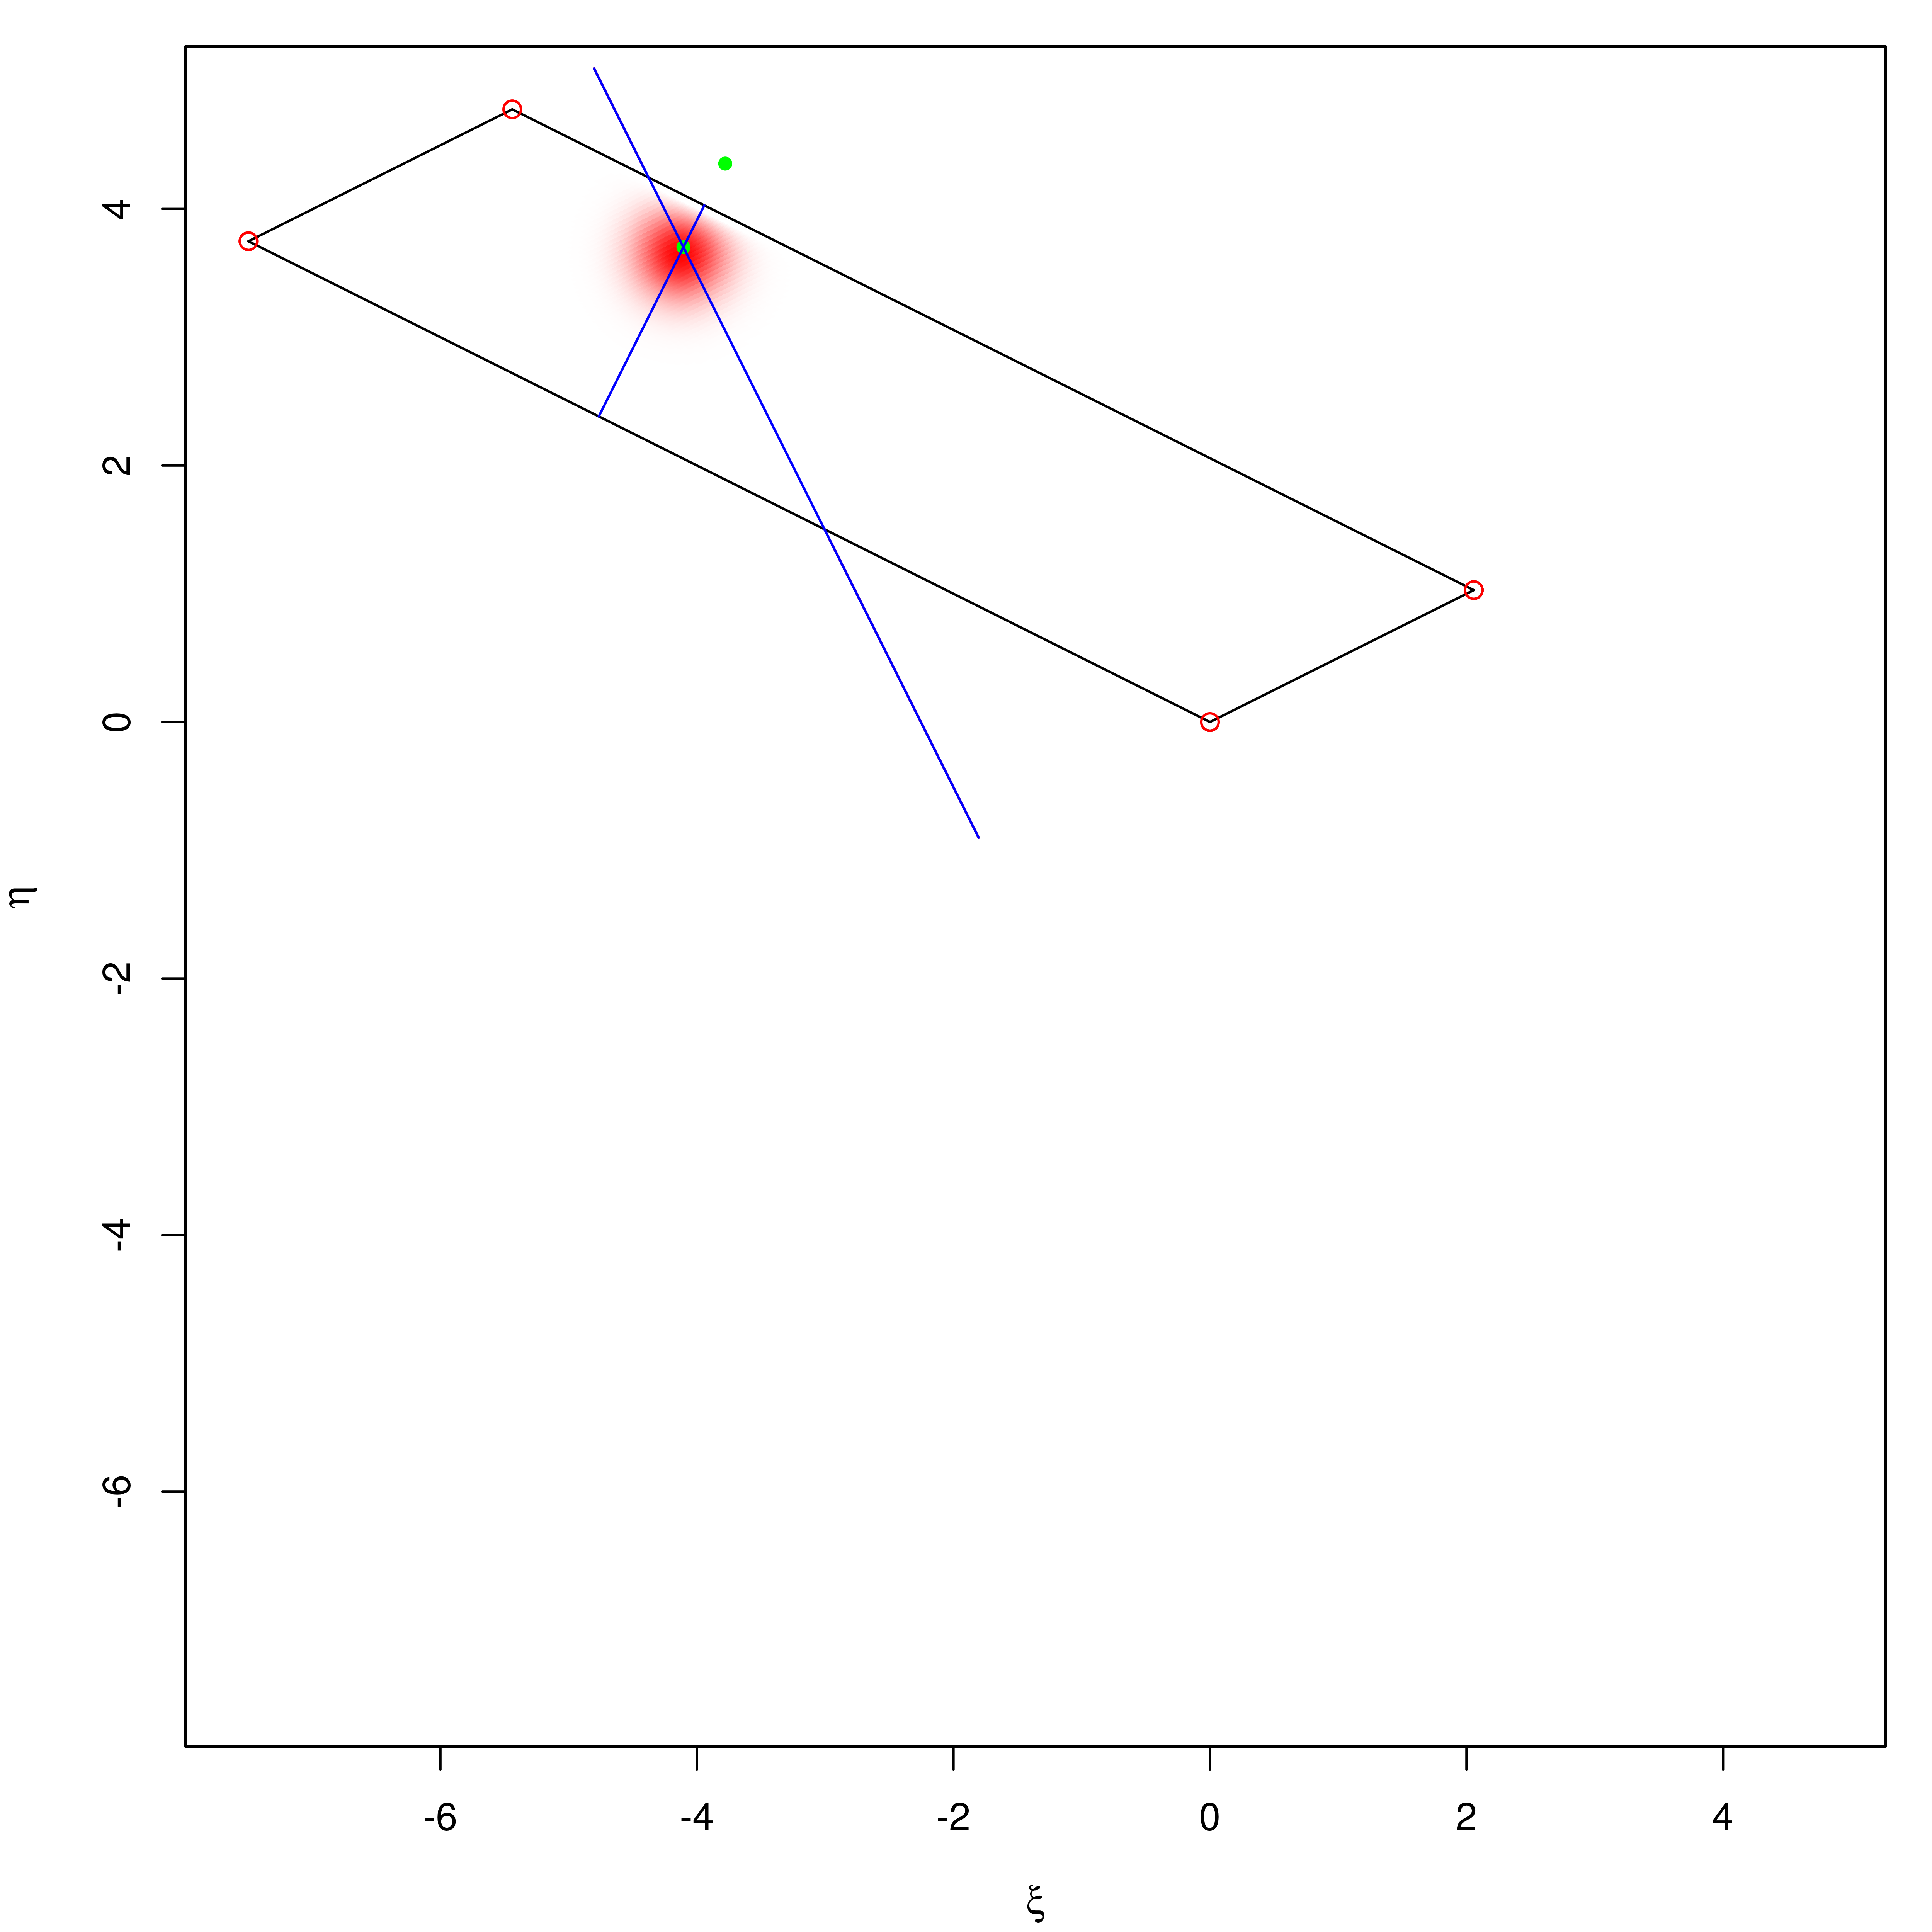
\includegraphics[width=1\linewidth]{../kernel-expansion/documentation/small-time-solution.png}
    \end{minipage}p
    %% 
    & \begin{minipage}{0.5\textwidth}
      \centering
      %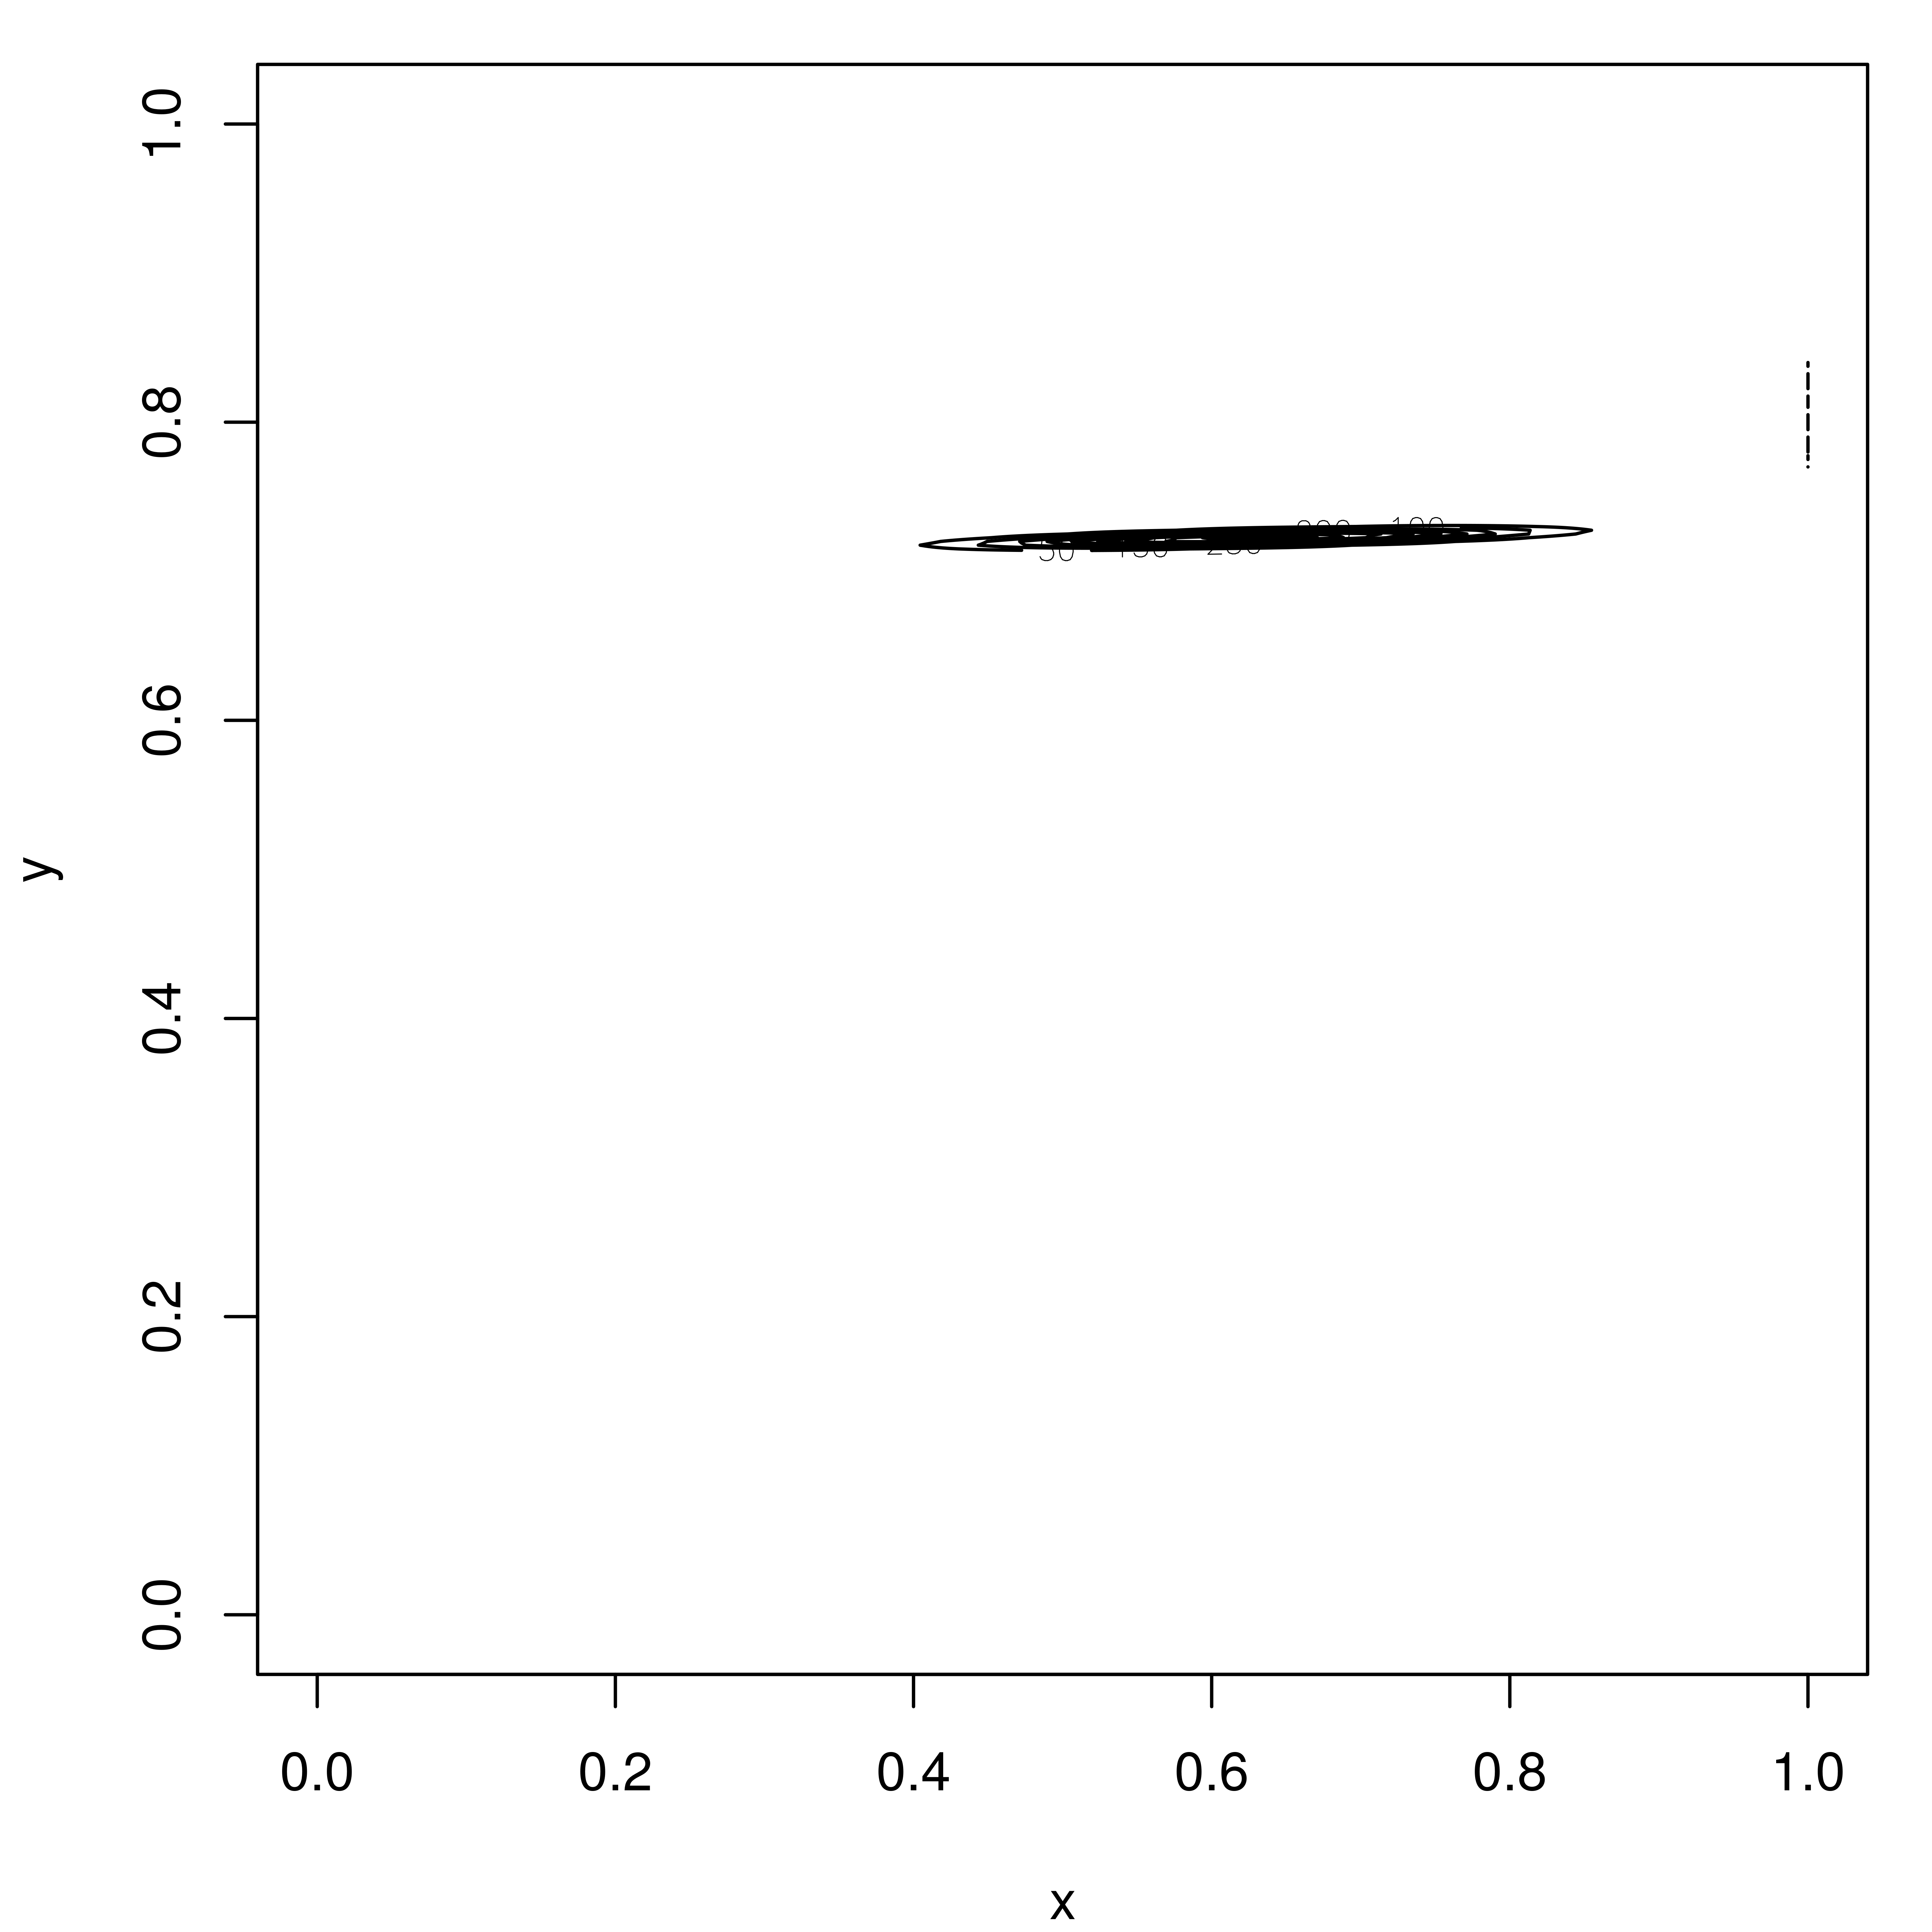
\includegraphics[width=1\linewidth]{../kernel-expansion/documentation/small-time-solution-contour.png}
    \end{minipage}
  \end{tabular}
  %%
  %%
  \caption{An example of the small-time solution
    $p(\xi,\eta,t_\epsilon)$ on the transformed domain
    $\tilde{\Omega}$ with $\tau_x = \tau_y = 1$ and $\rho=0.6$. Right:
    The shaded red region is a heatmap of the small-time solution in
    the transformed coordinate frame, while the blue line segments
    represent the distance between the boundaries and the initial
    condition coordinate. The green point outside of the computational
    domain is the center of the reflected image $(\xi_0', \eta_0')$
    about the closest boundary. Left: The small-time solution
    transformed back to the original coordinate system. Here, the
    contours denote the level-sets for the function. They very closely
    approximate the level sets for the fundamental solution of the
    unbounded problem (\ref{eq:qq})}
  \label{fig:step-1-small-time}
\end{figure}
Using Theorem 5.E of \cite{zeidler1995applied}, we can solve for
$p(x,y,t)$ by considering the smooth $p(x,y,t_\epsilon)$ as an initial
condition and evolving it forward in time by $t-t_\epsilon$. This
replaces initial condition orthogonality condition in
(\ref{eq:orthogonality-conditions-mat-2}) with
\begin{align}
  M \mathbf{c}(t_\epsilon) &= \mathbf{p}(t_\epsilon), \\
   [\mathbf{p}(t_\epsilon)]_i &= \displaystyle \int_\Omega p(x,y,t_\epsilon) \psi_i(x,y) dx\,dy. \nonumber
\end{align}
Intuitively, the bigger $t_\epsilon$, the smaller both $R_e(k)$ and
$R_0(k)$ will be, and the better our method will do.
% less eigenmodes present in $p(x,y,t_\epsilon)$, and the more accurate
% our weak solution according to the error estimate
% \[
%   \| e(t) \|_{L_2(\Omega)} \leq C h(k)^2 \| p(x,y,t_\epsilon) \|_{2}.
% \]


\subsection{Orthonormal Basis Family}
% An upper bound of the rate at which the Galerkin approximation
% converges to $p(x,y,t)$ is given by condition (\ref{eq:ic-bound}),
% namely by how well the initial condition may be approximated via a
% projection onto $S_k$.
We motivate the construction of the orthonormal basis functions by
once again considering the fundamental solution for the unbounded
problem (\ref{eq:qq}). In the absence of boundaries, (\ref{eq:qq}) is
solved by the function
\[
  G(x,y,t | x_0', y_0') = \frac{1}{2\pi\,\,t\,\, \tau_x\tau_y\sqrt{1-\rho^2}} \exp\left\{ -\frac{1}{2\,t(1-\rho^2)} \left( \frac{(x - x_0')^2}{\tau_x^2} - 2\rho \frac{(x-x_0')(y-y_0')}{\tau_x\tau_y} + \frac{(y - y_0')^2}{\tau_y^2}\right) \right\},
\]
with
$x_0' = (x_0 - a_x)/(b_x-a_x),\quad y_0' = (y_0 - a_y)/(b_y-a_y)$. We
choose the family of basis functions
$S_k = \left\{\psi_i(x,y), \,\, 0 \leq i \leq k \right\}$
\begin{align}
  \psi_i(x,y) &= \frac{1}{2\pi \sigma^2\sqrt{1-\tilde{\rho}^2} } \exp\left\{ -\frac{1}{2(1-\tilde{\rho}^2)\sigma^2} \left( (x - x_i)^2 - 2\tilde{\rho} (x-x_i)(y-y_i) + (y - y_i)^2 \right) \right\} x\left(1-x\right)\, y(1-y)
\end{align}
for some parameters $(\tilde{\rho}, \sigma)$ and a collection of nodes
$\{ (x_i,y_i) \}_{i=0}^k$ which form a grid over $\Omega$.

This grid is determined by the choice of kernel parameters
$(\tilde{\rho}, \sigma)$ with a scaling parameter $l$, and it is
defined in the following way. For $(\tilde{\rho}, \sigma, l)$, overlay
a grid $\{ (x'_j, y'_j) \}_{j=0}^{k'}$ such that
$(x'_0, y'_0) = (0.5,0.5)$ and the subsequent grid points are
$l\sigma(1 + \tilde{\rho})$ units apart in the $x-$direction and
$l\sigma(1 - \tilde{\rho})$ units apart in the $y-$direction over
$[1/2 - 1/\sqrt{2}, 1/2 + 1/\sqrt{2}] \, \times [1/2 - 1/\sqrt{2}, 1/2
+ 1/\sqrt{2}]$ (see left panel of Figure (\ref{fig:grids})).
%%
%%
\begin{figure}
  \centering
  %%
  %%
  \begin{tabular}{cc}
    \begin{minipage}{0.4\textwidth}
      \centering
      %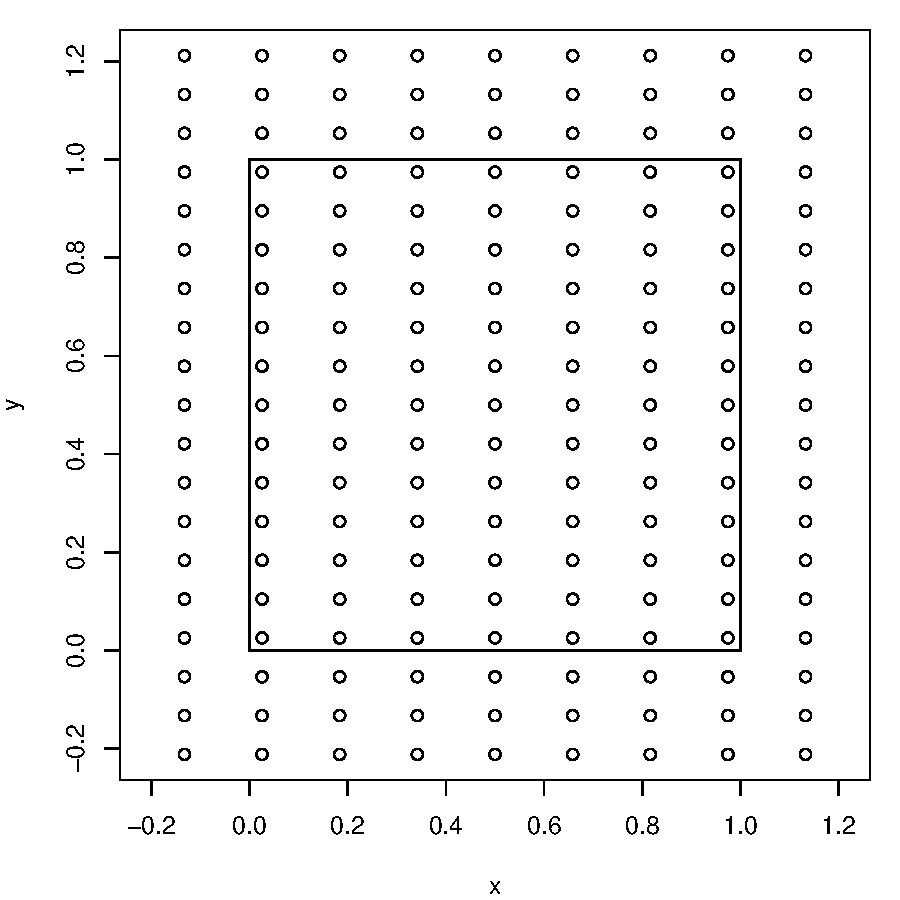
\includegraphics[width=1\linewidth]{../kernel-expansion/documentation/nodes-1.pdf}
    \end{minipage}
    %% 
    & \begin{minipage}{0.4\textwidth}
      \centering
      %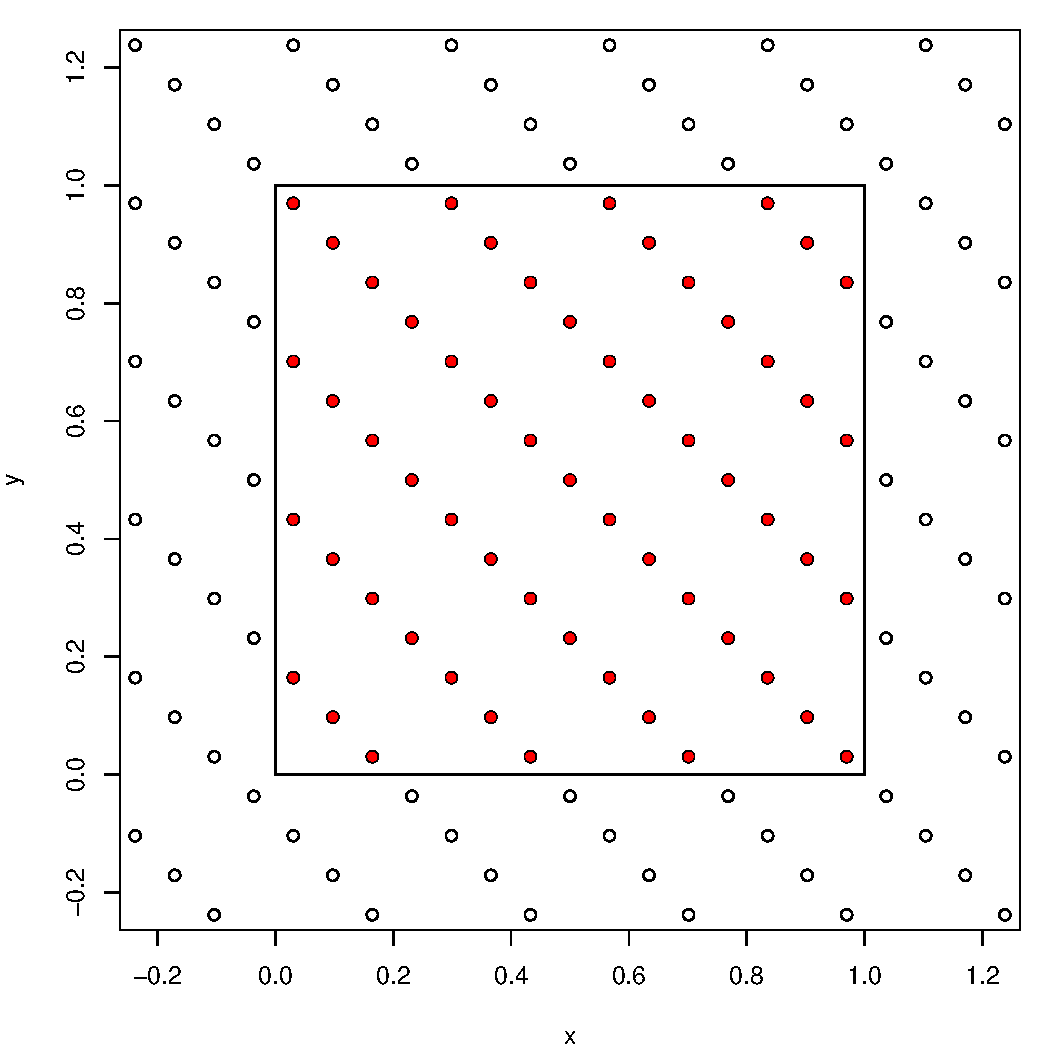
\includegraphics[width=1\linewidth]{../kernel-expansion/documentation/nodes-2.pdf}
    \end{minipage}
  \end{tabular}
  %%
  %%
  \caption{A sample grid design for $l=1$, $\sigma=0.3$ and $\rho=0.6$. The
    left panel corresponds to the initial grid
    $\{ (x'_j,y'_j) \}_{j=0}^{k'}$ over $\Omega$ (solid black
    square). The right panel depicts the rotated initial grid. The set
    of final node points $\{ (x_i,y_i) \}_{i=0}^{k}$ is contained
    within $\Omega$ and is denoted by the red solid points.}
  \label{fig:grids}
\end{figure}
%%
%%
Next, apply the clockwise, $\pi/4$ rotation centered on
$(1/2, 1/2)$ to each node
\begin{align*}
  \left( \begin{array}{c}
           x_j \\
           y_j
         \end{array} \right) =
       \left( \begin{array}{cc}
                1/\sqrt{2} & 1/\sqrt{2} \\
                -1/\sqrt{2} & 1/\sqrt{2}
              \end{array} \right) 
            \left( \begin{array}{c}
                     x'_j - 1/2\\
                     y'_j -1/2
                   \end{array} \right) +
  \left( \begin{array}{c}
           1/2 \\ 1/2
           \end{array} \right).
\end{align*}
The grid is comprised of all nodes within $\Omega$:
$\left\{(x_i, y_i)\right\}_{i=0}^k = \left\{ (x_j, y_j) | (x_j, y_j)
  \in \Omega, j = 0, \ldots, k' \right\}$ (see right panel of Figure
(\ref{fig:grids})). It should be noted that the level sets of the heat
kernel for the basis functions are ellipses with major and minor axes
aligned with the node points. Further, there is more resolution
(ie. the node layout is denser) along the direction corresponding to
the smaller standard deviation of the basis heat kernel in the
principal coordinate frame. Finally, for a given $l$, nodes in either
principal direction are separated by $l$ standard deviations of the
basis heat kernel. This layout naturally takes into account some
degree of correlation $\tilde{\rho}$ so that the small-time solution,
having level sets similar to those of the kernels, can be better
resolved. Essentially, the collection
$\{ \psi_i(x,y| \tilde{\rho}, \sigma) \}_{i=0}^k$ is composed of
fundamental solutions to a heat diffusion problem tuned by $\sigma$
and $\tilde{\rho}$, tampered such that their support is on $\Omega$,
zero on the boundaries, still smooth, and inheriting the correlation
structure of the fundamental solution to the problem. More basis
elements are added by decreasing $\sigma$ and altering $l$, while the
degree of correlation is controlled by $\tilde{\rho}$. For
the purposes of this paper, we found that keeping fixed $l=1$ with a
moderate $\tilde{\rho}$ ($|\tilde{\rho}| \sim 0.6$) yields reasonable
results. It is important, however, that
$\mbox{sign}(\tilde{\rho}) = \mbox{sign}(\rho)$ so that the
problematic, narrow component of the small-time solution (which can be
seen in the minor axis of the contours of the small-time solution in
the right panel of Figure (\ref{fig:step-1-small-time})) can be
resolved.

%
%In this manner,
% our basis function choice is in keeping with the golden rule for the
% rate of convergence: \textbf{The smoother the solution to the original
%   problem and the smoother the functions in the basis space, the
%   faster the convergence of the Ritz-Galerkin method.} (Remark 1(c) in
%   Chapter 2 of \cite{zeidler1995applied}).

At this point, having explicitly defined
$\psi_i(x,y|\sigma,\tilde{\rho})$, it should be noted that these basis
functions are constant with respect to the normalized problem
parameters $(\tau_x, \tau_y, \rho)$. Thus, the derivative of Galerkin
approximation $p^{(k)}$ with respect to the boundaries takes on the
form
\[
  \frac{\partial^4}{\partial a_x \partial b_x \partial a_y \partial
    b_y} p^{(k)}(x,y,t) = \boldsymbol{\psi}(x,y)^T
  \frac{\partial^4}{\partial a_x \partial b_x \partial a_y \partial
    b_y} \left\{ \exp\left( M^{-1}S\, t \right) \mathbf{c}(0) \right\},
\]
which is well-defined given the discussion above.

\subsection{Error Bound} \label{sec:error-bound}
A bound on the closeness of the approximate solution $p^{(k)}(x,y,t)$
to the strong solution $p(x,y,t)$ is developed in
\cite{bramble1977some}.  Their result shows that the Galerkin
approximation we use converges to the strong solution in
$L_2(\Omega)$, and it motivates the thrust of our numerical
solution. First, we define the \textit{error} term
\[
  e^{(k)}(t) = p(x,y,t) - p^{(k)}(x,y,t),
\]
as well as the norm
\[
  \| w \|_2 = \sum_{j=0}^\infty \lambda_j^2 \left<w, \phi_j\right>^2
\]
for the eigenpairs $(\lambda_j, \phi_j)$ of the operator
$\mathcal{L}$. As referred to in \cite{bramble1977some}, functions
$w \in L_2(\Omega)$ with $\|w\|_2 < \infty$ are also in
$W_2^2(\Omega)$. Finally, if we have the condition (corresponding to
equation 2.1 in \cite{bramble1977some})
\begin{align}
  \| p(x,y,t_\epsilon) - p^{(k)}(x,y,t_\epsilon) \|_{L_2(\Omega)} &\leq C\, h(k)^2 \| p(x,y,t_\epsilon) \|_2, \label{eq:ic-bound}
\end{align}
where $h(\cdot)$ is a decreasing function of $k > 0$, Theorem 2.1 in
\cite{bramble1977some} applies and we have the error estimate
\begin{align}
  \| e^{(k)}(t) \|_{L_2(\Omega)} \leq C h(k)^2 \| p(x,y,t_\epsilon) \|_{2}. \label{eq:error-est}
\end{align}
Here, the  constant $C$  and the  function $h(k)$ are  the same  as in
(\ref{eq:ic-bound}). The implication is that if the basis functions in
$S_k$ represent  the small-time  solution $p(x,y,t_\epsilon)$  with no
error, the Galerkin solution forward in time is also without error.

We can ensure condition (\ref{eq:ic-bound}) is met if $S_k$ is
complete in $L_2(\Omega)$ as $k$ grows. The other two conditions
necessary for the error bound to apply are demonstrated by
\cite{bramble1977some} for the Galerkin method. Equation
(\ref{eq:error-est}) can be summarized in a simple way: the
\textit{error} of the method is controlled by how much variation the
small-time solution has; the \textit{rate} of decrease of the error is
controlled by how well the span of $S_k$ represents the small-time
solution compared to the variation of the initial condition as $k$
increases. In the context of (\ref{eq:error-est}), our method, with
its small-time analytic solution and choice of basis functions, is
specifically tailored to minimize the error between the strong
solution and its Galerkin approximation under $L_2(\Omega)$.

% However, the initial condition for (\ref{eq:qq}) requires all in
% eigenmodes being included in the representation of the initial
% conditions, so that
% \[
%   \| p(x,y,0) \|_{2} = \left\| \delta\left( x - \frac{x_0 - a_x}{b_x-a_x}
%   \right) \delta\left( y - \frac{y_0 - a_y}{b_y-a_y} \right)\right\|_{2} = +\infty.
% \]
% It is obvious that we cannot apply the error estimates above. However,
% evolving the solution forward in time, even for a short period,
% diffuses the delta-function IC and attenuates out the highest
% frequency modes. Further, because solutions to the diffusion equation
% are smooth, $p(x,y,t_\epsilon)$ will give us a smooth initial function
% which will make the error bounds admissible.


\section{Estimation}
Consider the problem of estimating the parameters
$(\mu_x, \mu_y, \sigma_x, \sigma_y, \rho)$ from an i.i.d. set of
samples $(Z_1, \ldots, Z_n)$ from random variable $Z(t)$ at a given
value of $t$ in the process in (1)-(2). Specifically, $Z(t)$ is formed
as
$$ Z(t) =( X(t), Y(t), m_x(t), M_x(t), m_y(t), M_y(t)) $$
where 
$$m_x(t)= \min_{0 \le t' \le t} X(t), \;\; 
M_x(t)= \max_{0 \le t' \le t} X(t), \;\; m_y(t)= \min_{0 \le t' \le t}
Y(t), \;\; M_y(t)= \max_{0 \le t' \le t} Y(t). $$ We say that $Z_i$ is
sampled from the distribution corresponding to the probability density
function (\ref{eq:pdf})
\[
  Z_i \sim F(\theta),
\]
where the cumulative distribution function $F$ has the usual interpretation
\begin{align*}
  F(z = (x, y, a_x, b_x, a_y, b_y) | \theta) &= \Pr\left(X(t) \leq x,
    Y(t) \leq y, m_x \leq a_x, M_x \leq b_x, m_y \leq a_y, M_y \leq b_y\right).
\end{align*}

This estimation problem is of particular importance in quantitative
finance where the model equations (\ref{eq:X}) - (\ref{eq:Y}) (with
various bells and whistles attached) are widely used. However, to the
best of our knowledge, all current \textit{likelihood} methods in the
literature either ignore the observed maximum/minimum information or
use only some of it. Likelihood-free approaches, like that of
\cite{rogers1991estimating}, on the other hand suffer from not being
able to be easily integrated into inferential frameworks that require
explicit estimates of probability.

Since we do not have a closed-form solution for the likelihood, we
will use an iterative derivative-free maximization algorithm (the
Nelder-Mead method; see \cite{lagarias1998convergence} for review and
convergence properties) which requires repeated evauluation of the
likelihood. For moderate to large samples sizes this is feasible,
because our numerical method is specifically designed for
computational efficiency for repeatedly evaluating the density
function (\ref{eq:pdf}). The maximum likelihood estimator (MLE) for
the true parameters based on $n$ samples, which we call
$\hat{\theta}_n := (\hat{\mu}_x, \hat{\mu}_y, \hat{\sigma}_x,
\hat{\sigma}_y, \hat{\rho})$, is especially useful in practical
settings when it exhibits \textit{consistency}, \textit{i.e.}: the MLE
gets closer to the true parameter vector $\theta$ as more data is
collected and included in the likelihood (assuming the model and its
parameters remain constant during the data collection). More
precisely, the estimator $\hat{\theta}_n$ is consistent if it
converges in probability to the true parameter:
\[
  \Pr( | \hat{\theta}_n - \theta | ) \to 0 \qquad \mbox{as} \qquad n \to \infty.
\]

\subsection{Consistency}
In this section we prove that the MLE based on the Galerkin
approximation $p^{(k)}(x,y,t)$ to the governing Fokker-Planck equation
(\ref{eq:1}) is consistent. To do so, we first show that the
distribution on $Z$ based on the approximate $p^{(k)}(x,y,t)$ converges to
the true distribution $F(\cdot | \theta)$. Define the probability densities
\begin{align}
  f(z) &= f(x,y,a_x,b_x,a_y,b_y) := \Pr\left(X(t) \in dx, Y(t) \in dy, m_x \in da_x,
         M_x \in db_x, m_y \in da_y, M_y \in db_y \left| \theta \right.\right) \label{eq:stong-density} \\
    f^{(k)}(z) &= f^{(k)}(x,y,a_x,b_x,a_y,b_y) := \frac{\partial^4}{\partial a_x \partial b_x \partial a_y \partial
         b_y} q^{(k)}(x,y,t | a_x, b_x, a_y, b_y). \label{eq:galerkin-density}
\end{align}
The function $f(z)$ is the probability density function corresponding
to $q(x,y,t)$, the strong solution to the governing Fokker-Planck
equation; $f^{(k)}(z)$ corresponds to the approximate solution
$q^{(k)}$ of the unnormalized equation obtained from the Galerkin
approximation $p^{(k)}$ of the normalized equation. Before proceeding,
we should note that both $f(z)$ and $f^{(k)}(z)$ exist. So see the
case for $f(z)$, consider the relation
\begin{align*}
  &f(x,y,a_x,b_x,a_y,b_y) = \\
  &\Pr\left(X(t) \in dx, Y(t) \in dy, m_x \in da_x, M_x \in db_x, m_y
  \in a_y, M_y \in db_y \left| \theta \right.\right) = \\
  &\mathbb{P}_{W}\left( \underbrace{\left\{ \omega \in W \left| X_\omega(t) = x,
  Y_\omega(t)=y, \inf_{t'\in [0,1]} X_\omega(t') = a_x,
  \sup_{t'\in [0,1]} X_\omega(t') = b_x, \inf_{t'\in [0,1]}
        Y_\omega(t') = a_y, \sup_{t'\in [0,1]} Y_\omega(t') = b_y
      \right. \right\}}_{A(x,y,a_x,b_x,a_y,b_y) = A(z)}\right)
\end{align*}
where $\mathbb{P}_{W}$ is the Wiener measure on the sample space $W$
of all realizations (paths) $(X_\omega(t), Y_\omega(t))$ from the
stochastic process (\ref{eq:X}) - (\ref{eq:Y}) defined in the usal way
using Kolmogorov's extension of measure over cylinder sets on
$t \to \mathbb{R}^2$ (see \cite{freidlin1985functional}, Section
1.2). Sets of the form $A(x,y,a_x,b_x,a_y,b_y)$ can be defined as a
countable intersection/union of cyliner sets on $t \to \mathbb{R}^2$,
hence they are measurable under $\mathbb{P}_{W}$; therefore $f(z)$ exists and
is bounded above by 1. Moreover, since $q(x,y,t|a_x,b_x,a_y,b_y)$ represents the
integral of $f(z)$ with respect to the boundary variables, we have
\[
  f(x,y,a_x,b_x,a_y,b_y) = \frac{\partial^4}{\partial a_x \partial b_x \partial a_y \partial
         b_y} q(x,y,t | a_x, b_x, a_y, b_y).
\]
The existence of $f^{(k)}(z)$ as defined in
(\ref{eq:galerkin-density}) is guaranteed by Theorem 4.1 in
\cite{singler2008differentiability}. The result states that weak
solutions to parabolic problems are differentiable with respect to
parameters as long as the weak (Galerkin-form) operator
$\left< \mathcal{L} \psi_i(x,y), \psi_j(x,y) \right>$ is
differentiable with respect to the parameters. The condition certainly
holds for the normalized problem (\ref{eq:qq}) with our choice of
basis functions $S_k$, as they are infinitely differentiable with
repsect to $x,y$, the boundaries, and the diffusion parameters. 

At this point we will assume that for a sufficiently large $k$,
$f^{(k)}(z)$ is positivie for all $z \in Z$ and is integrable over
$Z$. As such, we may regard it as a proper probability density
function with the cumulative probability density and probability
measure over $Z$ being 
\begin{align}
  F^{(k)}(z | \theta) &= \displaystyle \int_{-\infty}^{a_x} \displaystyle \int_{-\infty}^{a_y} \displaystyle \int_{-\infty}^{b_x} \displaystyle \int_{-\infty}^{b_y} \displaystyle \int_{-\infty}^x \displaystyle \int_{-\infty}^y \frac{\partial^4}{\partial a'_x \partial b'_x \partial a'_y \partial b'_y} q^{(k)}(x', y', t | a'_x, b'_x, a'_y, b'_y)\,\,\, dx'\, dy'\, da'_x\, db'_x\, da'_y\, db'_y, \label{eq:approx-measure} \\
                          \Pr_{k}(A) &:= \displaystyle \int_{A} f^{(k)}(z)\, dz, \quad \mbox{ for any measurable } A \subset Z. \label{eq:approx-measure-2}
\end{align}
We will prove that for every $z \in Z$,
\[
  \lim_{k\to \infty} F^{(k)}(z | \theta) = F(z | \theta).
\]
First, we prove the Lemma
\begin{lemma}\label{lem:1}
  For $z = (x, y, a_x, b_x, a_y, b_y)$,
  \[
    \lim_{k\to \infty} \displaystyle \int_{a_x}^{b_x} \displaystyle
    \int_{a_y}^{b_y} f^{(k)}(x,y,a_x,b_x,a_y,b_y)\, dx\,dy =
    \displaystyle \int_{a_x}^{b_x} \displaystyle \int_{a_y}^{b_y}
    f(x,y,a_x,b_x,a_y,b_y)\, dx\,dy.
  \]
\end{lemma}
\begin{proof}
  Define the sets of form, for $z = (x,y,a_x,b_x,a_y,b_y)$,
  \begin{align*}
    B(a_x, b_x, a_y, b_y) &= \left\{ z' \in Z \left| z' \in [a_x, b_x]
        \times [a_y, b_y] \times [a_x, \infty) \times (-\infty, b_x]
                            \times [a_y, \infty) \times (-\infty, b_y] \right.\right\}.
  \end{align*}
  Elements within $B(a_x, b_x, a_y, b_y)$ are equivalent to sample paths that stay within the region $[a_x, b_x] \times [a_y, b_y]$:
  \begin{align*}
    B(a_x, b_x, a_y, b_y) &= \left\{ \omega \in W | X_\omega(t) \in [a_x, b_x], Y_\omega(t) \in [a_y, b_y], m_x \in [a_x,b_x), M_x \in (a_x, b_x] \right\}
  \end{align*}

  Then
  \begin{align}
    \Pr(B(a_x, b_x, a_y, b_y)) &= \displaystyle \int_{B(a_x, b_x, a_y, b_y)} f(z)\, dz \nonumber \\ 
                               &= \displaystyle \int_{a_x}^{\infty} \displaystyle \int_{-\infty}^{b_x} \displaystyle \int_{a_y}^{\infty} \displaystyle \int_{-\infty}^{b_y} \displaystyle \int_{-\infty}^{b_x} \displaystyle \int_{-\infty}^{b_y} f(x', y', a'_x, b'_x, a'_y, b'_y) dx' dy' da_x' db_x' da_y' db_y' \label{eq:full-form} \\
                               &= \displaystyle \int_{a_x}^{b_x} \displaystyle \int_{a_y}^{b_y} q(x,y,a_x,b_x,a_y,b_y)\, dx\, dy, \nonumber
  \end{align}
  
  where the last equality employs the interpretation of $q$ in
  (\ref{eq:CDF}) and we can freely change the order of integration as
  $f$ is bounded for all $z \in Z$. Similarly,
  \begin{align*}
    \Pr_k(B(a_x, b_x, a_y, b_y)) &= \displaystyle \int_{a_x}^{b_x} \displaystyle \int_{a_y}^{b_y} q^{(k)}(x,y,a_x,b_x,a_y,b_y)\, dx\, dy.
  \end{align*}
  From (\ref{eq:full-form}), the partial derivative of the probability
  $\Pr(B(a_x,b_x,a_y,b_y))$ is well-defined and can be written as
  \begin{align*}
    \frac{\partial^4}{\partial a_x \partial b_x \partial a_y \partial b_y} \Pr(B(a_x, b_x, a_y, b_y)) &= \displaystyle \int_{a_x}^{b_x} \displaystyle \int_{a_y}^{b_y} f(x,y,a_x,b_x,a_y,b_y)\, dx\, dy.
  \end{align*}
  The second-order \textbf{finite difference} approximation the above
  expression can be expressed as a linear combination of probabilities
  of perturbed sets $B(\cdot)$:
  \begin{align*}
    \lim_{\epsilon \to 0}\quad \frac{1}{\epsilon^4} \sum_{i=1}^{16} c(i) \Pr(B(a_x + k_1(i)\epsilon, b_x + k_2(i)\epsilon, a_y + k_3(i)\epsilon, b_y + k_4(i)\epsilon) &= \\
    \MoveEqLeft[8] \frac{\partial^4}{\partial a_x \partial b_x \partial a_y \partial b_y} \Pr(B(a_x, b_x, a_y, b_y)),
  \end{align*}
  where $c$ and $k$ are functions from $i$ to the appropriate
  coefficients in the second-order finite difference approximation
  $c(i) \to \left\{-1, 1\right\}$, $k_j(i) \to \{-1,1\}$. Using Big-O
  notation, for a sufficiently small $\epsilon$
  \begin{align}
    \sum_{i=1}^{16} c(i) \Pr(B(a_x + k_1(i)\epsilon, b_x +
    k_2(i)\epsilon, a_y + k_3(i)\epsilon, b_y + k_4(i)\epsilon) &= \nonumber \\
    \MoveEqLeft[10] \epsilon^4 \frac{\partial^4}{\partial a_x \partial b_x \partial
      a_y \partial b_y} \Pr(B(a_x, b_x, a_y, b_y)) + O(\epsilon^6 ;
    a_x, b_x, a_y, b_y). \label{eq:fin-diff}
  \end{align}
  The convergence result in Section \ref{sec:error-bound} implies that
  \begin{align*}
    \Pr_k(B(a_x + k_1(i)\epsilon, b_x + k_2(i)\epsilon, a_y +
    k_3(i)\epsilon, b_y + k_4(i)\epsilon) &= \\
    \MoveEqLeft[10] \displaystyle \int_{a_x +
    k_1(i)\epsilon}^{b_x + k_2(i)\epsilon} \displaystyle \int_{a_y + k_3(i)\epsilon}^{b_y +
    k_4(i)\epsilon} q^{(k)}(x,y,a_x,b_x,a_y,b_y)\, dx\, dy \to \\
   \displaystyle
     \int_{a_x + k_1(i)\epsilon}^{b_x + k_2(i)\epsilon} \displaystyle \int_{a_y +
     k_3(i)\epsilon}^{b_y + k_4(i)\epsilon} q(x,y,a_x,b_x,a_y,b_y)\, dx\, dy &= \\
    \MoveEqLeft[20] \Pr(B(a_x + k_1(i)\epsilon, b_x + k_2(i)\epsilon, a_y +
    k_3(i)\epsilon, b_y + k_4(i)\epsilon) \mbox{ as } k \to \infty \mbox{ in } L_2(\Omega).
  \end{align*}
  Hence, for a sufficiently large $k$ dependent on the supremum over
  $i$, and given the error estimate in (\ref{eq:error-est}), we have
  the relation
  \begin{align*}
    \Pr_k(B(a_x + k_1(i)\epsilon, b_x + k_2(i)\epsilon, a_y +
    k_3(i)\epsilon, b_y + k_4(i)\epsilon) &= \\
    \Pr(B(a_x + k_1(i)\epsilon, b_x + k_2(i)\epsilon, a_y +
    k_3(i)\epsilon, b_y + k_4(i)\epsilon) &\\
    + O(h(k)^2; a_x + k_1(i)\epsilon, b_x + k_2(i)\epsilon, a_y + k_3(i)\epsilon, b_y + k_4(i)\epsilon) &
  \end{align*}
  Note here that the dominating terms $O(h(k)^2; \cdot)$ are
  differentiable with respect to the boundary parameters
  $(a_x, b_x, a_y, b_y)$ since $q$ and $q^{(k)}$ have this
  property. Therefore, if we replace $\Pr(\cdot)$ in
  (\ref{eq:fin-diff}) with $\Pr_k(\cdot)$
  \begin{align*}
    \sum_{i=1}^{16} c(i) \Pr_k(B(a_x + k_1(i)\epsilon, b_x +
    k_2(i)\epsilon, a_y + k_3(i)\epsilon, b_y + k_4(i)\epsilon) &= \\
    \sum_{i=1}^{16} c(i) \Pr(B(a_x + k_1(i)\epsilon, b_x +
    k_2(i)\epsilon, a_y + k_3(i)\epsilon, b_y + k_4(i)\epsilon) &  \\
    + \sum_{i=1}^{16} c(i) O(h(k)^2; a_x + k_1(i)\epsilon, b_x +
    k_2(i)\epsilon, a_y + k_3(i)\epsilon, b_y + k_4(i)\epsilon) &= \\
    \epsilon^4 \frac{\partial^4}{\partial a_x \partial b_x \partial
    a_y \partial b_y} \Pr(B(a_x, b_x, a_y, b_y)) + O(\epsilon^6 ;
    a_x, b_x, a_y, b_y) & \\
    + \sum_{i=1}^{16} c(i) O(h(k)^2; a_x + k_1(i)\epsilon, b_x +
    k_2(i)\epsilon, a_y + k_3(i)\epsilon, b_y + k_4(i)\epsilon). &
  \end{align*}
  Dividing both sides by $\epsilon^4$ produces
  \begin{align*}
    \frac{1}{\epsilon^4} \sum_{i=1}^{16} c(i) \Pr_k(B(a_x + k_1(i)\epsilon, b_x +
    k_2(i)\epsilon, a_y + k_3(i)\epsilon, b_y + k_4(i)\epsilon) &= \frac{\partial^4}{\partial a_x \partial b_x \partial
                                                                  a_y \partial b_y} \Pr(B(a_x, b_x, a_y, b_y)) + O(\epsilon^2;
                                                                  a_x, b_x, a_y, b_y) \\
                                                                &+ \frac{1}{\epsilon^4}\sum_{i=1}^{16} c(i) O(h(k)^2; a_x + k_1(i)\epsilon, b_x +
                                                                  k_2(i)\epsilon, a_y + k_3(i)\epsilon, b_y + k_4(i)\epsilon) \\
    % = \frac{\partial^4}{\partial a_x \partial b_x \partial
    % a_y \partial b_y} \Pr(B(a_x, b_x, a_y, b_y)) + O(\epsilon;
    % a_x, b_x, a_y, b_y) + \frac{\partial^4}{\partial a_x \partial b_x \partial
    % a_y \partial b_y} O(h(k)^2 ; a_x, b_x, a_y, b_y)
  \end{align*}
  As mentioned above $O(h(k)^2; \cdot)$ is differentiable with respect
  to the boundary parameters, so that the right-most term is still
  $O(h(k)^2)$ as $\epsilon \to 0$. Taking the limit in $\epsilon$, we have
  \begin{align*}
    \displaystyle \int_{a_x}^{b_x} \displaystyle \int_{a_y}^{b_y}
    f^{(k)}(x,y,a_x,b_x,a_y,b_y)\, dx\, dy =
    \frac{\partial^4}{\partial a_x \partial b_x \partial a_y \partial
    b_y} \Pr_k(B(a_x, b_x, a_y, b_y)) \\
    = \frac{\partial^4}{\partial
      a_x \partial b_x \partial a_y \partial b_y} \Pr(B(a_x, b_x, a_y,
    b_y)) +  O(h(k)^2; a_x, b_x, a_y, b_y) \\
    =\displaystyle \int_{a_x}^{b_x} \displaystyle \int_{a_y}^{b_y}
    f(x,y,a_x,b_x,a_y,b_y)\, dx\, dy + O(h(k)^2; a_x, b_x, a_y, b_y).
  \end{align*}
  Therefore, we have the desired result:
  \[
    \lim_{k\to \infty} \displaystyle \int_{a_x}^{b_x} \displaystyle
    \int_{a_y}^{b_y} f^{(k)}(x,y,a_x,b_x,a_y,b_y)\, dx\,dy =
    \displaystyle \int_{a_x}^{b_x} \displaystyle \int_{a_y}^{b_y}
    f(x,y,a_x,b_x,a_y,b_y)\, dx\,dy.
  \]
\end{proof}

\begin{lemma}[Convergence in distribution] \label{lem:conv-dist}
  For any $z \in Z$,
  $ \lim_{k \to \infty} F^{(k)}(z | \theta) = F(z).$

\end{lemma}

\begin{proof}
  Let
  $I^{(k)}(z) = \displaystyle \int_{a_x}^{x} \displaystyle
  \int_{a_y}^{y} f^{(k)}(u,v,a_x,b_x,a_y,b_y)\, du\,dv$ and let
  $I(z) = \displaystyle \int_{a_x}^{x} \displaystyle \int_{a_y}^{y}
  f(u,v,a_x,b_x,a_y,b_y)\, du\,dv$. It is possible to show that
  $\lim_{k\to \infty} I^{(k)}(z) = I(z)$ as a consequence of Lemma
  \ref{lem:1} by considering some $\chi_k(z) \in S_k$ approximating
  the indicator $1(u \leq x, v \leq y)$ as $k \to \infty$ and setting up a triangle
  inequality. However, we will omit this technical detail here.

  Next, we know that $I(z)$ is integrable over $(a_x, b_x, a_y, b_y)$
  as $\Pr(Z) = \mathbb{P}_{W}(W) = 1$. The Dominated Convergence
  Theorem applies, and we therefore have
  \[
    \lim_{k \to \infty} \displaystyle \int_{-\infty}^{a_x} \displaystyle \int_{-\infty}^{b_x} \displaystyle \int_{-\infty}^{a_y} \displaystyle \int_{-\infty}^{b_y} I^{(k)}(z) da_x' db_x' da_y' db_y' = \displaystyle \int_{-\infty}^{a_x} \displaystyle \int_{-\infty}^{b_x} \displaystyle \int_{-\infty}^{a_y} \displaystyle \int_{-\infty}^{b_y} I(z) da_x' db_x' da_y' db_y',
  \]
  which implies the result of the Lemma.
\end{proof}
% \begin{align*}
%   q(x,y,t) = \\
%   \Pr\left(X(t) \in dx, Y(t) \in dy,  \min_{t'}X(t') \geq a_x,
%   \max_{t'}X(t')\leq b_x, \min_{t'} Y(t')\geq a_y, \max_{t'} Y(t')\leq b_y|  X(0)=x_0, Y(0)=y_0, \theta \right) = \\
%   \Pr_{W}\left(\left\{ \omega \in \Omega | X_\omega(t) \in dx,\,\, Y_\omega(t) \in dy,\,\,  \forall t' \in [0,t]\,\, a_x \leq X_\omega(t') \leq b_x,\,\, \forall t' \in [0,t] \,\, a_b \leq Y_\omega(t') \leq b_y,\,\, X_\omega(0) = Y_\omega(0) = 0 \right\} \right)
% \end{align*}
% Our strategy will be to define a family of sets $\left\{ \tilde{A}_m(z) \right\}_{m=0}^\infty$ for any $z=(x,y,a_x,b_x,a_y,b_y)$ such that
% \begin{align*}
%   \lim_{m \to \infty} \Pr_W \left(  \tilde{A}_m(z) \right) = 
%   \Pr \left( X(t) \leq x,
%   Y(t) \leq y, \min_{t' \leq t} X(t') \leq a_x, \max_{t' \leq t}
%   X(t') \leq b_x, \min_{t' \leq t} Y(t') \leq a_y, \max_{t' \leq t}
%   Y(t') \leq b_y \right) = F(z | \theta)
% \end{align*}

% \begin{lemma}
%   For $z = (x,y,a_x,b_x,a_y,b_y)$, 
%   \[\lim_{m \to \infty} \displaystyle \int_{-\infty}^x \displaystyle
%     \int_{-\infty}^y q(x',y',t, a_x-m, b_x, a_y-m, b_y)\,\, dx'\,dy' -
%     \displaystyle \int_{-\infty}^x \displaystyle \int_{-\infty}^y
%     q(x',y',t, a_x, b_x, a_y, b_y)\,\, dx'\,dy' = F(z | \theta)\]
% \end{lemma}
% \begin{proof}
% Given some $z = (x,y,a_x,b_x,a_y,b_y)$, define the sets
% \begin{align*}
%   A_m(z) &= \left\{ \omega \in \Omega | X_\omega(t) \leq x,\,\,
% Y_\omega(t) \leq y,\,\, \right. \\ & \forall t' \in [0,t]\,\, a_x-m
% \leq X_\omega(t') \leq b_x,\,\, \\ & \forall t' \in [0,t] \,\, a_y -
% m\leq Y_\omega(t') \leq b_y,\,\, \\ & \left.X_\omega(0) = Y_\omega(0)
% = 0 \right\}, \quad \quad m = 0,1,2,... \\
% \end{align*}
% Note here that $\Pr_{W}(A_m(z)) = \displaystyle \int_{-\infty}^x \displaystyle \int_{-\infty}^y q(x',y',t, a_x-m, b_x, a_y-m, b_y)\,\, dx'\,dy'$.  Next, we define
% \begin{align*}
%   \tilde{A}_{m}(z) &= A_m(z) \,\, \bigcap \,\, A_0^C(z) \\
%                    &= \left\{ \omega \in \Omega | X_\omega(t) \in dx,\,\, \right.\\
%                    & \quad \quad \forall t' \in [0,t]\,\, a_x-m \leq X_\omega(t') \leq b_x,\,\, \\
%                    & \quad \quad \forall t' \in [0,t] \,\, a_y - m\leq Y_\omega(t') \leq b_y,\,\, \\
%                    & \quad \quad \exists t_{a_x} \in [0,t] \,\, s.t. \,\, X_\omega(t_{a_x}) < a_x \,\, , \exists t_{a_y} \in [0,t] \,\, s.t. \,\, X_\omega(t_{a_y}) < a_y, \\
%                    & \quad \quad \left.X_\omega(0) = Y_\omega(0) = 0 \right\}
% \end{align*}
% It is easy to see that $A_{m}(z) \subset A_{m+1}(z)$ and that
% $\tilde{A}_{m}(z) \subset \tilde{A}_{m+1}(z)$. Because of the former
% relation,
% \[
%   \Pr_{W}(\tilde{A}_m(z)) = \Pr_W(A_m(z)) - \Pr_{W}(A_0(z)) = \displaystyle \int_{-\infty}^x \displaystyle \int_{-\infty}^y q(x',y',t, a_x-m, b_x, a_y-m, b_y)\,\, dx'\,dy' - \displaystyle \int_{-\infty}^x \displaystyle \int_{-\infty}^y q(x',y',t, a_x, b_x, a_y, b_y)\,\, dx'\,dy'.
% \]
% Finally,
% \begin{align*}
%   \bigcup_{m=0}^\infty \tilde{A}_m(z) &= \left\{ \omega \in \Omega | X_\omega(t) \in dx,\,\, \right.\\
%                    & \quad \quad \forall t' \in [0,t]\,\, -\infty \leq X_\omega(t') \leq b_x,\,\, \\
%                    & \quad \quad \forall t' \in [0,t] \,\, -\infty \leq Y_\omega(t') \leq b_y,\,\, \\
%                    & \quad \quad \exists t_{a_x} \in [0,t] \,\, s.t. \,\, X_\omega(t_{a_x}) < a_x \,\, , \exists t_{a_y} \in [0,t] \,\, s.t. \,\, X_\omega(t_{a_y}) < a_y, \\
%                    & \quad \quad \left.X_\omega(0) = Y_\omega(0) = 0 \right\},
% \end{align*}
% such that for $\omega \in \bigcup_{m=0}^\infty \tilde{A}_m(z)$,
% $X_\omega(t) \leq x, Y_\omega(t) \leq y, \min_{t'} X_{\omega}(t') \leq
% a_x, \min_{t'} Y_{\omega}(t') \leq a_y, \max_{t'} X_{\omega}(t') \leq
% b_x$, $\max_{t'} Y_{\omega}(t') \leq b_y$, and
% \[
%   \Pr_W\left( \bigcup_{m=0}^\infty \tilde{A}_m(z) \right) = \lim_{M \to \infty} \Pr_W\left( \bigcup_{m=0}^M \tilde{A}_M(z) \right) = F(z |
%   \theta).
% \]
% Since $\tilde{A}_{m}(z) \subset \tilde{A}_{m+1}(z)$,
% \[
%   \lim_{m\to \infty} \Pr_W(\tilde{A}_m(z)) = \lim_{m \to \infty} \displaystyle \int_{-\infty}^x \displaystyle \int_{-\infty}^y q(x',y',t, a_x-m, b_x, a_y-m, b_y)\,\, dx'\,dy' - \displaystyle \int_{-\infty}^x \displaystyle \int_{-\infty}^y q(x',y',t, a_x, b_x, a_y, b_y)\,\, dx'\,dy'  = F(z | \theta)
% \]
% \end{proof}
% For a shorthand, denote
% $
%   \mu_k(\tilde{A}_m(z)) = \displaystyle \int_{-\infty}^x \displaystyle \int_{-\infty}^y q_k(x',y',t, a_x-m, b_x, a_y-m, b_y)\,\, dx'\,dy' - \displaystyle \int_{-\infty}^x \displaystyle \int_{-\infty}^y q_k(x',y',t, a_x, b_x, a_y, b_y)\,\, dx'\,dy'.
% $

% \begin{lemma} \label{lem:weak}
%   For a fixed $m$, $\mu_k(\tilde{A}_m(z)) \to \Pr_W(\tilde{A}_m(z))$ as $k\to \infty$.
% \end{lemma}
% \begin{proof}
%   The proof for this lemma follows direcly from the convergence result
%   $p^{(k)} \to p$ as $k\to \infty$ under the $L_2(\Omega)$ norm from
%   Section \ref{sec:semidiscrete-galerkin}.
% \end{proof}
% With the result from Lemma \ref{lem:weak}, we can now define the
% function $k(m; z)$ as
% \[
%   k(m; z) := \inf_{k'}\left\{ \left| \mu_{k'}(\tilde{A}_m(z)) - \Pr_W(\tilde{A}_m(z)) \right| < 1/2m  \right\}
% \]

% \begin{lemma}\label{lem:convergence-in-dist}
%   For $F_{k(m;z)}$, $F$, and $z$ defined above,
%   \[ \lim_{m\to \infty} F_{k(m;z)}(z | \theta) = F(z | \theta). \]
% \end{lemma}

% \begin{proof}
%   For any $\epsilon > 0$, let $M_1 = 2/\epsilon$. By Lemma
%   \ref{lem:1}, we can find $M_2$ such that $\forall m > M_2$
%   $\left| \Pr_W(\tilde{A}_m(z) - F(z | \theta) \right| <
%   \epsilon/2$. Let $M = \max\{M_1, M_2\}$. For any $m > M$,
%   \begin{align*}
%     \left| F_{k(m)}(z) - F(z) \right | &= \left| \mu_{k(m)}(\tilde{A}_m(z)) - F(z) \right | \\
%                                        &\leq \left|  \mu_{k(m)}(\tilde{A}_m(z)) - \Pr_W(\tilde{A}_m(z)) \right| + \left|  \Pr_W(\tilde{A}_m(z)) - F(z | \theta) \right|. \\
%                                        &\leq \epsilon/2 + \epsilon/2
%   \end{align*}
%   The left term bound is defined by $k(m;z)$.
% \end{proof}

% % \begin{lemma}
% %   For a fixed $k$,
% %   $\lim_{m\to \infty} \mu_k(\tilde{A}_m(z)) = c \in \mathbb{R},$ i.e.
% %   $\left\{ \mu_k(\tilde{A}_m(z))\right\}_{m=0}^\infty$ is a convergent
% %   sequence.
% % \end{lemma}

% % \begin{proof}[Proof idea]
% %   Here we will present a formal argument, without giving all of the
% %   necessary technical details. As $m \to \infty$, the parameters
% %   $\tau_x, \tau_y$ in the normalized problem are $O(1/m)$.  Further,
% %   the initial condition coordinates tend to
% %   $((1-1/m),(1-1/m))$. Letting $\gamma = 1/m$ for $m >> 1$, the
% %   normalized problem becomes
% %   \begin{equation*}
% %     \frac{\partial}{\partial t} p(x,y,t) = \mathcal{L}p(x,y,t),\quad (x,y) \in = \Omega
% % \end{equation*}
% % with the initial condition
% % \begin{align*}
% %   p(x,y,0) &= \delta\left( x - (1-\gamma) \right) \delta\left(y-(1-\gamma)\right),
% % \end{align*}
% % where the differential operator $\mathcal{L}$ is of order
% % \[
% %   \mathcal{L} = \frac{1}{2} \gamma^2 \frac{\partial^2}{\partial x^2}
% %   + \rho\gamma^2 \frac{\partial^2}{\partial x \partial y} + \frac{1}{2}\gamma^2 \frac{\partial^2}{\partial y^2}.
% % \]
% % This means that fundamental solution to the unbounded problem above is
% % the Gaussian density
% % \[
% %   G(x,y,t'| \gamma) = \frac{1}{2\pi\,\,t'\,\, \gamma^2\sqrt{1-\rho^2}} \exp\left\{ -\frac{1}{2\, t' \, (1-\rho^2)} \left( \frac{(x - 1 + \gamma)^2}{\gamma^2} - 2\rho \frac{(x-1+\gamma)(y-1+\gamma)}{\gamma^2} + \frac{(y - 1 + \gamma)^2}{\gamma^2}\right) \right\}, t' \in (0,t]
% % \]
% % We claim that according to our method, we can find a constant $\Gamma$
% % such that for $\gamma < \Gamma$, $t_\epsilon > t$ for the small-time
% % solution $p(x,y,t_\epsilon)$, which means that $G(x,y,t | \gamma)$
% % solves the above problem. This means that, \textbf{for fixed} $k$, the
% % Galerkin approximation generated by our method is the projection of
% % $p(x,y,t)$ onto the basis family $S_k$ (there is no forward evolution
% % of the problem).

% % Further, because
% % $G(x,y,t | \gamma) \to \delta(x-1+\gamma)\delta(y-1+\gamma)$ weakly as
% % $\gamma \to 0$, each of the projections of $G(x,y,t | \gamma)$ onto $S_k$ converge to the basis functions evaluated at $((1-\gamma), (1-\gamma))$:
% % \[
% %   \displaystyle \int_\Omega G(x,y,t | \gamma) \psi_i(x,y) dx\,dy \to \psi_i(1-\gamma,1-\gamma).
% % \]
% % Given $S_k$, the above coefficients uniquely define $p^{(k)}$
% % projection is defined only by $p(x,y,t_\epsilon)$ and $S_k$ only on
% % $\mathbf{p}(t_\epsilon)$ (see equation
% % (\ref{eq:orthogonality-conditions-mat-2})) become the same. Because
% % $k$ is fixed, the mass $M$ stays the same, which means that the
% % initial condition vectors in the Galerkin method also converge at
% % $\gamma \to 0$. Fu
% % \end{proof}

\begin{lemma}
  The maximum likelihood estimator is consistent as $n \to \infty$ and $m \to \infty$:
  \[ \hat{\theta}_{n,k} \to \theta \].
\end{lemma}
\begin{proof}
  By Lemma \ref{lem:conv-dist}
    \[ Z_k \xrightarrow[]{d} Z \mbox { as } k \to \infty. \] Next,
    given Theorem 4.1 in \cite{singler2008differentiability}, we know
    that, for each $k$, $q_k$ is analytic in both the diffusion
    parameters and boundary parameters. Hence, the probability density
    function satisfies the criteria A1 - A6 in
    \cite{casella2002statistical} to guarantee that, for data
    $Z_{k} \sim F_k(\theta)$,
    \[ \hat{\theta}_{n,k}(Z_k) \xrightarrow[]{p} \theta \mbox{ as } n
      \to \infty. \]

    Now we need to show that the same holds for data sampled from $F$
    as $k \to \infty$. To do this, we will use Chebyshev's inequality:
  \[
    \Pr_{Z}\left( \left| \hat{\theta}_{n,k}(Z) - \theta \right| \geq
      \epsilon \right) \leq \frac{ \mbox{E}_{Z}\left[
        (\hat{\theta}_{n,k}(Z) - \theta)^2 \right] }{ \epsilon^2 }.
  \]
  By the Maximum theorem [REFERENCE], $\hat{\theta}_{n,k}(x)$ is a continuous
  function with respect to $x$, and further because we have bounded
  $\hat{\theta}$ from below and above,
  \[
    \mbox{E}_{Z_k}\left[ (\hat{\theta}_{n,k}(Z_k) - \theta)^2 \right]
    \to \mbox{E}_{Z}\left[ (\hat{\theta}_{n,k}(Z) - \theta)^2 \right]
    \mbox{ as } k \to \infty
  \]
  by the portmanteau lemma. Finally, we can show that
  \begin{equation}
    \mbox{E}_{Z_k}\left[ (\hat{\theta}_{n,k}(Z_k) - \theta)^2 \right]
    \to 0 \mbox{ as } n \to \infty, \label{eq:var-lim}
  \end{equation}
  since the expected value of the estimator tends to $\theta$ and its
  variance goes to 0 when $n \to \infty$. Therefore, given any
  $\epsilon > 0$ and $\delta > 0$, we can find a sufficiently large
  $n$ and $k$ such that
  \[
    \Pr_{Z}\left( \left| \hat{\theta}_{n,k}(Z) - \theta \right| \geq
      \epsilon \right) \leq \frac{ \mbox{E}_{Z}\left[
        (\hat{\theta}_{n,k}(Z) - \theta)^2 \right] }{ \epsilon^2 } < \delta    
  \]
\end{proof}

\subsection{Simulation Study}
Next we present some numerical simulation results for the Galerkin
method. The finite-difference step used to derive the likelihood
function is of size $\Delta = 1/16$ with the $\mathcal{O}(\Delta^2)$
order accuracy. If the inital/final condition is forced outside of the
computation domain, the $\mathcal{O}(\Delta)$ finite difference
approximation is used instead. The inner products that need to be
computed to establish the system of equations for the method are
computed using the trapezoidal rule on a regular $400 \times 400$
grid.

Data is generated from the model with zero drift via forward
Euler discretization where the obtained discrete-time extrema are
recorded and used as the realized extrema of the process. We use 500
data sets, each comprised of 128 simulations generated with the same
parameters
\[
  \mu_x = 0,\quad \mu_y  = 0,\quad \sigma_x = 1,\quad \sigma_y = 1,\quad \rho = 0.6.
\]
The drift parameters are assumed known, so that the MLE is comprised
of the diffusion and correlation parameters:
$\hat{\theta} = (\hat{\sigma}_x, \hat{\sigma}_y, \hat{\rho}).$ For
each dataset, the MLE found is a sample from the repeated-sampling
distrubtion for $\hat{\theta}$. Results are compared to the
repeated-sampling distribution of the MLE based on the usual bivariate
normal likelihood which does not take into account the
boundaries. Results are shown in Figure (\ref{fig:mle-comparison}),
including the root-mean-square-errors of the two estimators.

\begin{figure}
  \centering
  %%
  %%
  \begin{tabular}{ccc}
    \begin{minipage}{0.3\textwidth}
      \centering
      %\includegraphics[width=1\linewidth]{../kernel-expansion/documentation/mle-comparison-sigma-x.pdf}
    \end{minipage}
    %% 
    & \begin{minipage}{0.3\textwidth}
      \centering
      %\includegraphics[width=1\linewidth]{../kernel-expansion/documentation/mle-comparison-sigma-y.pdf}
    \end{minipage}
    & \begin{minipage}{0.3\textwidth}
      \centering
      %\includegraphics[width=1\linewidth]{../kernel-expansion/documentation/mle-comparison-rho.pdf}
    \end{minipage}
  \end{tabular}
  \caption{Kernel-density plots of the MLE samples obtained from the
    Galerkin likelihood (blue) and the classical likelihood
    (green). The data-generating parameters are denoted with the
    vertical solid line. The root-mean-square errors for the pairs of
    estimators are included. As expected, the Galerkin-based
    likelihood outperforms the Gaussian likelihood for each
    parameter.}
  \label{fig:mle-comparison}
\end{figure}


\chapter{Analytically Resolving the Transient Region of the Galerkin Solution}
\label{ch:small-time}

% In this chapter we have established the existence of an approximate,
% analytic solution for small values of $t$ whose applicability is
% well defined in terms of error rates at the boundaries (BCs) and the
% locations of the images (ICs).
Chapter \ref{ch:galerkin} introduced a semidiscrete (finite element)
Galerkin method for solving the standardized diffusion problem
(\ref{eq:qqq}). The Galerkin method is most appropriate for moderate
to large times, since numerical errors are attenuated with increasing
diffusion time $\tilde{t}$. Further, numerical simulations
demonstrated the need to resolve the likelihood function for small
$\tilde{t}$ in order to fully use the information present in OCHL
data. We will call this parameter rage the \textit{incomputable
  region} of the Galerkin solver. For parameters in the incomputable
region, a sufficient condition to flag them as such is if the
numerical derivative of the finite element solution with respect to
the boundary parameters produces a negative value. However, this is
not a \textit{necessary} condition, and in practice this is an
insidious problem: parameter combinations which should be attributed
with a very small likelihoods may be given values orders of magnitude
higher than they should and thus bias any inferential procedure (see
Figure \ref{fig:limitations-rho-0.95-1} in Chapter \ref{ch:galerkin})
for an illustration). In this chapter, we develop an analytic solution
applicable in a small-$\tilde{t}$ region. In addition to having its
own well-defined criteria for appropriate use (namely an upper bound
on $\tilde{t}$ as well as an upper bound on $\tilde{\sigma}$). In this
chapter we also develop an analytic matching solution that bridges the
small-$\tilde{t}$ solution and the Galerkin solution across the
transient $\tilde{t}$ region. 

\section{A small-time solution to the PDE, revisited}
As part of the overall Galerkin method, Chapter \ref{ch:galerkin}
introduced a small-time approximation for the normalized diffusion
problem \eqref{eq:qqq} via the method of images (see Section
\ref{sec:pde-small-t}). By reflecting the fundamental solution
(i.e. the solution to the governing PDE without the boundary conditions) about the
closest boundary and picking a sufficiently small
$\tilde{t}_\epsilon$, the sum of images function \eqref{eq:p-epsilon}
\begin{align}
  p_\epsilon(\tilde{x}, \tilde{y}, \tilde{t}) &= G(\tilde{x}, \tilde{y}, \tilde{t} | \tilde{x}_0, \tilde{y}_0) - G(\tilde{x}, \tilde{y}, \tilde{t} | \tilde{x}'_0, \tilde{y}'_0)
\end{align}
satisfies the initial condition, the governing PDE, and the boundary
conditions. However, because the analytic dependence of this
small-time approximation on the boundaries is only through the
location parameters $(\tilde{x}'_0, \tilde{y}'_0)$ of the single
reflected image, differentiating with respect to all four boundaries
yields a uniform zero value in computing the transition density
$\frac{\partial^4}{\partial a_x \partial b_x \partial a_y \partial
  b_y} p(\tilde{x}, \tilde{y}, \tilde{t})$.

\subsection{Uniqueness and Symmetry Condition}
The insufficiency of the previous small-time solution suggests
extending the system of images by performing more than a single
reflection. If there exists an image whose location is the
result of at least one reflection about each of the four boundaries,
then this image is guaranteed to have a non-trivial contribution to
the density
$\frac{\partial^4}{\partial a_x \partial b_x \partial a_y \partial
  b_y} p(\tilde{x}, \tilde{y}, \tilde{t})$. An immediate problem with
the extension, however, is the uniqueness of the resultant approximate
density function. To illustrate the problem, consider the two systems
of images constructed by carrying out the series of reflections
\begin{align}
  & R_1 := \left\{ 1,2,3,4 \right\}, & R_2 := \left\{ 2,3,4,1 \right\}, & \label{eq:reflection-sets}
\end{align}
where $\left\{ r_i, r_j, r_k, r_l \right\}$ denotes the set of images
generated by the following steps
\begin{enumerate}
\item $r_i:$ Reflect the initial condition
  $(\tilde{x}_0, \tilde{y}_0)$ abour boundary $r_i$ to produce
  coordinate $(\tilde{x}_{r_i}, \tilde{y}_{r_i})$. The system of
  images consists of locations
  \begin{align*}
    \left\{(\tilde{x}_0, \tilde{y}_0), (\tilde{x}_{r_i},
  \tilde{y}_{r_i})\right\}
  \end{align*}
  with signs $\left\{1, -1\right\}$.
\item $r_j:$ Reflect each of $\left\{(\tilde{x}_0, \tilde{y}_0), (\tilde{x}_{r_i},
  \tilde{y}_{r_i})\right\}$ about boundary $r_j$ and add to existing set of images to produce
  \begin{align*}
    \left\{ (\tilde{x}_0, \tilde{y}_0), (\tilde{x}_{r_i},
    \tilde{y}_{r_i}), (\tilde{x}_{r_j}, \tilde{y}_{r_j}), (\tilde{x}_{r_j, r_i},
    \tilde{y}_{r_j, r_i}) \right\}
  \end{align*}
  with signs $\left\{1,-1,-1,1\right\}$.

\item $r_k:$ Reflect each of $\left\{ (\tilde{x}_0, \tilde{y}_0), (\tilde{x}_{r_i},
    \tilde{y}_{r_i}), (\tilde{x}_{r_j}, \tilde{y}_{r_j}), (\tilde{x}_{r_j, r_i},
    \tilde{y}_{r_j, r_i}) \right\}$ about boundary $r_k$ and add to existing set of images to produce
  \begin{align*}
    & \left\{ (\tilde{x}_0, \tilde{y}_0), (\tilde{x}_{r_i},
    \tilde{y}_{r_i}), (\tilde{x}_{r_j}, \tilde{y}_{r_j}), (\tilde{x}_{r_j, r_i},
    \tilde{y}_{r_j, r_i}), \right. & \\
    & \left. (\tilde{x}_{r_k}, \tilde{y}_{r_k}), (\tilde{x}_{r_k, r_i},
    \tilde{y}_{r_k, r_i}), (\tilde{x}_{r_k, r_j}, \tilde{y}_{r_k, r_j}), (\tilde{x}_{r_k, r_j, r_i},
    \tilde{y}_{r_k, r_j, r_i})  \right\}&
  \end{align*}
  with signs $\left\{1,-1,-1,1, -1,1,1,-1\right\}$.
\item $r_l:$ Reflect each of the existing image locations about
  boundary $r_l$ and add to the existing set of images.
\end{enumerate}
Here, boundary $1$ corresponds to $\tilde{y}=0$, boundary 2 to
$\tilde{x}=1$, boundary 3 to $\tilde{y}=1$, and boundary 4 to
$\tilde{x} = 0$.  Given the set $\left\{r_i,r_j,r_k,r_l\right\}$, we
re-define $p_\epsilon$ as the the sum of all $J = 16$ images
\begin{equation*}
  p_\epsilon(\tilde{x}, \tilde{y}, \tilde{t}) = \sum_{j=1}^J (-1)^{n(j)}
  G(\tilde{x},\tilde{y},\tilde{t}|\tilde{x}_{(j)},\tilde{y}_{(j)}),
\end{equation*}
where $n(j)$ is the number of reflections performed to produce image
$j$, and $(\tilde{x}_{(j)},\tilde{y}_{(j)})$ is the $j^{th}$ image
location in the sequence at the end of Step 4 above. The newly defined
$p_\epsilon$ analytically satisfies the boundary condition at $r_l$
(since it is the last reflection), and it also satisfies the PDE. Once
again we can choose a sufficiently small $\tilde{t}_\epsilon$ such
that the boundary conditions at $r_i, r_j,$ and $r_k$ hold numerically
as well.

Referring back to the example reflection sets in
\eqref{eq:reflection-sets}, although not identical, the two solutions
to the PDE problem corresponding to $R_1$ and $R_2$ have minimal
relative differences, and they depart from the true analytic solution
minimally. From a numerical implementation standpoint, there is only
near machine-$\varepsilon$ difference between them. However, the two
solutions have a single image,
$(\tilde{x}_{1,2,3,4}, \tilde{y}_{1,2,3,4})$ and
$(\tilde{x}_{2,3,4,1}, \tilde{y}_{2,3,4,1})$ respectively, whose
location is a function of all four boundaries, and this single image
entirely defines the corresponding density function
$\frac{\partial^4}{\partial a_x \partial b_x \partial a_y
  \partial b_y}p_\epsilon$. Because the location parameters of these images are
different, the joint densities of $(x_0, y_0, x, y, a_x, b_x, a_y, b_y)$
derived from the two PDE solutions are consequently very different as
well. Uniqueness of the solution using the method of images is
achieved by performing an infinite number of reflections, which is not
always possible (see Section \ref{sec:proof} below).

A condition weaker than uniqueness which nonetheless restricts the
solution space is the symmetry obeyed by the problem. We consider the transformation
\begin{align}
  x^{new} = (a_x + b_x) - 2x^{old}, \\
  y^{new} = (a_y + b_y) - 2y^{old}.
\end{align}
The PDF solution to the initial-boundary problem of the diffusion
equation and joint density of $(x_0,y_0,x,y,a_x,b_x,a_y,b_y)$ are
invariant with respect to this transformation. In order for the sum of
images solution to obey this symmetry condition, the proposed system
of images must be preserved under the corresponding coordinate
transformation. Further, if we require that the system of images
contain the fewest possible elements, then the unique system of images
is the union of the sets of reflections
\begin{align}
  \left\{ 1,2,3,4 \right\} \cup \left\{ 2,3,4,1 \right\} \cup \left\{ 3,4,1,2 \right\} \cup \left\{ 4,1,2,3 \right\}. \label{eq:union}
\end{align}
When $(\tilde{x}_0, \tilde{y}_0) = (1/2,1/2)$, the set of
images from \eqref{eq:union} is closed under the transformation as
desired:
\begin{align*}
  \{1,2,3,4 \} & \to \{3,4,1,2 \}, \\
  \{2,3,4,1 \} &\to \{4,1,2,3 \}, \\
  \{3,4,1,2 \} &\to \{1,2,3,4 \}, \\
  \{4,1,2,3 \} &\to \{2,3,4,1 \}.
\end{align*}
Removing duplicate member images of \eqref{eq:union} and summing over
the remaining $J^* \leq 64$, we define the new small-time solution
\begin{equation}
  p_\epsilon(\tilde{x}, \tilde{y}, \tilde{t}) = \sum_{j=1}^{J^*} (-1)^{n(j)}
  G(\tilde{x},\tilde{y},\tilde{t}|\tilde{x}_{(j)},\tilde{y}_{(j)}). \label{eq:small-time-sol}
\end{equation}
We can control the relative error of the approximation by setting the
minimum absolute value of $p_\epsilon$ at the boundaries and solving
for $\tilde{t}_\epsilon$.
% For a boundary error rate of at most $1 \cdot 10^{-12}$, the
% solution based on the distribution bound by the symmetric (green)
% images from Figure (\ref{fig:illustration-1}) produces palatable
% relative errors across $\Omega$ compared to the true closed-form
% solution, as shown in Figure (\ref{fig:illustration-rel-error}) where
% the maximum relative error on a $30 \times 30$ grid is $O(10^{-5})$.
% Decreasing the error rate on the boundary to $1 \cdot 10^{-14}$ forces
% $t^* \approx 0.047$ and the max relative error on the same grid is
% $O(10^{-6})$.
%
% As in Chapter 2, we can scale,
% rotate, and scale again the problem, so that the boundaries of the
% computational domain have changed, but the fundamental solution to the
% problem is defined by an uncorrelated bivariate Gaussian distribution
% with variance $t$ in each direction. The transformed problem is shown
% in Figure (\ref{fig:transformed-problem-rho-0}).
% The topology under the transformed problem (under $T_{(3)}$ in
% \eqref{eq:T3}) permits the repeated reflection of the fundamental
% solution about the boundaries without any of the images falling within
% the computational domain $\Omega_3$. This further allows for
% subsequent images for fall further from the domain (scaling linearly
% in distance) so that there exists an asymptotic series composed of an
% infinite number of reflections which enforce the IC/BCs and satisfy
% the governing PDE.

\begin{figure}
  \centering
  %%
  %%
  \begin{tabular}{cc}
    \begin{minipage}{0.40\textwidth}
      \centering
      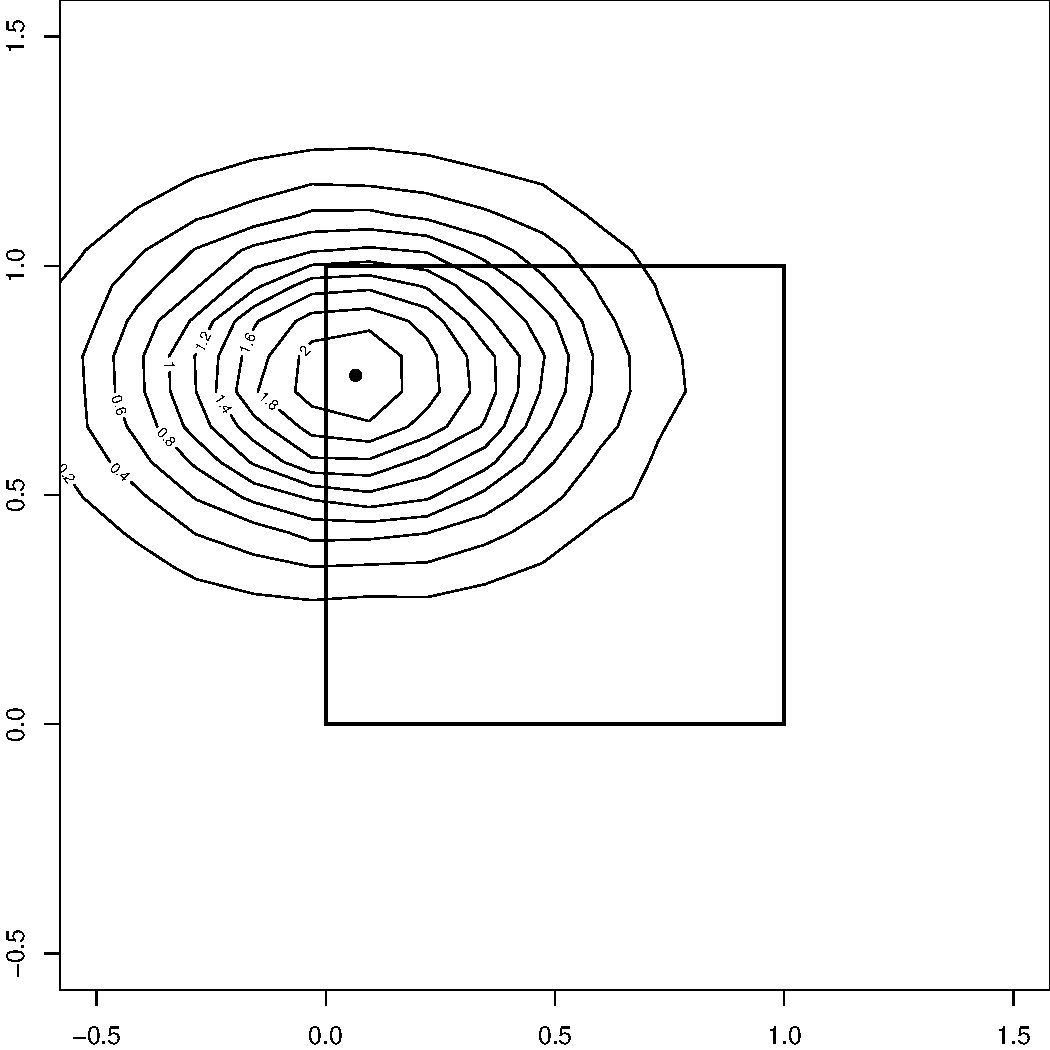
\includegraphics[width=1\linewidth]{../chapter-3/illustration-rho-0-normalized.pdf}
      \caption{The computational domain $\Omega_2$ for the normalized
        problem (\ref{eq:qqq}) is the unit square centered on
        $(0.5,0.5)$, shown in the figure as a square box. Level sets
        of the fundamental solution with $\rho = 0$ and
        $\sigma_{\tilde{y}} < 1$ are also shown at an initial
        condition in the upper-left corner of $\Omega_2$.}
      \label{fig:normalized-problem-rho-0}
    \end{minipage} &
    %%
    \begin{minipage}{0.40\textwidth}
      \centering
      \includegraphics[width=1\linewidth]{../chapter-3/illustration-rho-0-transformed.pdf}
      \caption{The problem in Figure
        \ref{fig:normalized-problem-rho-0} is scaled by
        $1/\tilde{\sigma}$ in the $y-$direction, then rotated $\pi/4$
        counter-clockwise, then scaled again in the principal axes
        direction in order to eliminate the mixing term in the
        resultant PDE problem. Since $\rho=0$ here, the final scaling
        is the identity transformation and the boundaries remain
        orthogonal. The fundamental solution is symmetric under
        rotations centered on the IC under the new topology, as shown
        here.}
      \label{fig:transformed-problem-rho-0}
    \end{minipage}
  \end{tabular}
\end{figure}

% We can compose such a finite system of images by reflecting about each
% of the boundaries a number of times and picking the greatest possible
% time $t^{*}$ such that all boundaries are either numerically or
% analytically enforced. One candidate for such a set of reflections is
% shown in Figure (\ref{fig:illustration-1}), where the set of images is
% produced by the reflections (left, right, left, top, bottom, top). The
% solid colored points are image positions having non-zero derivatives
% with respect to all four boundary parameters. The green points bound a
% symmetric solution respect to a family of transformations centered the
% IC (red).

\begin{figure}
  \begin{tabular}{cc}
    \begin{minipage}{0.40\textwidth}
      \centering
      \includegraphics[width=1\linewidth]{../chapter-3/chapter-3-figure-illustration-1.pdf}
      \caption{A finite system of images resultant from the sequence
        of reflections (left, right, left, top, bottom, top), where
        ``left'' refers to left boundary of $\Omega$ running along
        $x=0$, ``right'' refers to the right boundary along $x=1$,
        etc. The red point is the initial condition
        $(x_0,y_0) = (0.1, 0.3)$ which centers the fundamental
        solution. All points outside $\Omega$ are image position
        resulting from the reflections, where the solid colored points
        have positions dependent on $(x_0,y_0)$ \textit{as well as all
          of the boundaries.} The green colored points are symmetric
        about the IC with respect to horizontal and vertical
        reflections centered on $(x_0, y_0)$. The blue points are also
        dependent on all four boundaries, but they violate such
        transformations centered on $(x_0, y_0)$.}
      \label{fig:illustration-1}
    \end{minipage}
    %%
    & \begin{minipage}{0.40\textwidth}
      \centering
      \includegraphics[width=1\linewidth]{../chapter-3/chapter-3-figure-illustration-rel-error.pdf}
      \caption{Relative error across $\Omega$ on a $30 \times 30$
        regular grid based on solution (\ref{eq:small-time-sol}) for
        the symmetric distribution (green set) of images in Figure
        \ref{fig:illustration-1}. The max admissible small time
        $t^*$ is bounded above by $0.058$ and used here. The relative
        error rate is on the order of $0.01\%$}
      \label{fig:illustration-rel-error}
    \end{minipage}
      \end{tabular}
\end{figure}


\section{Calculation of the Joint Density}
Out of the $J^*$ images in \eqref{eq:small-time-sol}, exactly four
have location parameters dependent on all of the boundary parameters
$(a_x, b_x, a_y, b_y)$. Hence, the density calculation with the
small-time solution becomes
\begin{equation}
  \frac{\partial^4 p_\epsilon(\tilde{x}, \tilde{y}, \tilde{t})}{\partial a_x \partial b_x \partial a_y \partial b_y}  = \sum_{j'=1}^{4}
                                                                                                                        \frac{\partial^4G(\tilde{x},\tilde{y},\tilde{t}|\tilde{x}_{(j')},\tilde{y}_{(j')})}{\partial a_x \partial b_x \partial a_y \partial b_y}. \label{eq:derivs-1}
\end{equation}
One approach to compute the derivatives in (\ref{eq:derivs-1}) is to
numerically perturb the boundary parameters $(a_x,b_x,a_y,b_y)$ and
use a finite difference approximation directly on the sum
(\ref{eq:small-time-sol}). However, since the small-time solution
generally requires the use of a small time
$\tilde{t} \leq \tilde{t}_\epsilon \ll 1$, numerical underflow makes
direct application of finite difference hopeless.  We can, however,
leverage the very tractable analytic form of the Gaussian kernel
$G(\cdot)$ in \eqref{eq:Gfundamental} by defining the following
factors to more easily express the higher-order derivatives applied to
(\ref{eq:derivs-1})
\begin{align}
  \mathcal{C}(\tilde{t}, \sigma_{\tilde{y}}, \rho) &:= -\frac{1}{2\,\,\tilde{t}\, \sigma_{\tilde{y}}^2 (1-\rho^2)}, \\
  \mathcal{P}_j(\tilde{x},\tilde{y} | \tilde{x}_{(j)}, \tilde{y}_{(j)}) &:= \left(\tilde{x}- \tilde{x}_{(j)}\right)^2 \sigma_{\tilde{y}}^2 + \left(\tilde{y}-\tilde{y}_{(j)}\right)^2 - 2\rho(\tilde{x}-\tilde{x}_{(j)})(\tilde{y}-\tilde{y}_{(j)})\sigma_{\tilde{y}}.
\end{align}
The two key observations here are that $\mathcal{P}_j(\cdot)$ is
independent of $\tilde{t}$, meaning $\mathcal{C}(\cdot)$ carries the
$\tilde{t}$ dependency in differentiation and that only
$\mathcal{P}_j$ is dependent on the boundary parameters through
$\tilde{x}_{(j)}$ and $\tilde{y}_{(j)}$. Without loss of generality,
we can express the derivatives:
\begin{align}
  % \frac{\partial}{\partial a_x} G(x,y|t^{*}, \tilde{\sigma}, \rho, x_0^{(j^*)}, y_0^{(j^*)}) &= G \cdot \mathcal{C}\,\,\cdot \left( \frac{\partial \mathcal{P}}{\partial a_x} \right)\\
  % \frac{\partial^2}{\partial a_x \partial b_x} G(x,y|t^{*}, \tilde{\sigma}, \rho, x_0^{(j^*)}, y_0^{(j^*)}) &= G \cdot \mathcal{C}^2 \left( \frac{\partial \mathcal{P}}{\partial b_x} \right) \left( \frac{\partial \mathcal{P}}{\partial a_x} \right) + G \cdot \mathcal{C} \cdot \left( \frac{\partial^2 \mathcal{P}}{\partial a_x \partial b_x} \right) \\
  % %% %% %%
  % \frac{\partial^3}{\partial a_x \partial b_x \partial a_y} G(x,y|t^{*}, \tilde{\sigma}, \rho, x_0^{(j^*)}, y_0^{(j^*)}) &= G \cdot \mathcal{C}^3 \left( \frac{\partial \mathcal{P}}{\partial b_x} \right) \left( \frac{\partial \mathcal{P}}{\partial a_x} \right) \left( \frac{\partial \mathcal{P}}{\partial a_y} \right) \nonumber \\
  %                                                                                            &\,\, + G \cdot \mathcal{C}^2 \left[\left( \frac{\partial^2 \mathcal{P}}{\partial a_x \partial a_y} \right) \left( \frac{\partial \mathcal{P}}{\partial b_x} \right) + \left( \frac{\partial^2 \mathcal{P}}{\partial b_x \partial a_y} \right) \left( \frac{\partial \mathcal{P}}{\partial a_x} \right) + \left( \frac{\partial^2 \mathcal{P}}{\partial a_x \partial b_x} \right) \left( \frac{\partial \mathcal{P}}{\partial a_y} \right)\right] \nonumber \\
  %                                                                                            &\,\, + G \cdot \mathcal{C} \left( \frac{\partial^3 \mathcal{P}}{\partial a_x \partial b_x \partial a_y} \right) \nonumber \\
  %                                                                                            %% %% %%
  \frac{\partial^4}{\partial a_x \partial b_x \partial a_y \partial b_y} G(\tilde{x},\tilde{y},\tilde{t} |  \tilde{x}_{(j)}, \tilde{y}_{(j)}) &= \\
  \MoveEqLeft[10] G \cdot \mathcal{C}^4 \cdot \left(\partial_{a_x}\partial_{b_x} \partial_{a_y}\partial_{b_y} \right)\mathcal{P}&  \nonumber \\
  \MoveEqLeft[10] \,\, + G \cdot \mathcal{C}^3 \cdot \left( \partial^2_{a_x\, b_x} \partial_{a_y} \partial_{b_y} + \partial^2_{a_x\, a_y} \partial_{b_x} \partial_{b_y} + \partial^2_{a_x\, b_y} \partial_{b_x} \partial_{a_y} + \right. &\nonumber \\
  \MoveEqLeft[10] \left. \qquad\qquad\qquad +\partial^2_{b_x\, a_y} \partial_{a_x} \partial_{b_y} + \partial^2_{b_x\, b_y} \partial_{a_x} \partial_{a_y} \partial^2_{a_y\, b_y} \partial_{a_x} \partial_{b_x} \right) \mathcal{P} &  \nonumber \\
  \MoveEqLeft[10] \,\, + G \cdot \mathcal{C}^2 \cdot \left( \partial^3_{a_x\,b_x\,a_y} \partial_{b_y} + \partial^2_{a_x\,b_x}\partial^2_{a_y\,b_y} + \partial^3_{a_x\,b_x\,b_y}\partial_{a_y}  + \right.& \nonumber \\
  \MoveEqLeft[10] \left. \qquad\qquad\qquad + \partial^3_{a_x\,a_y\,b_y} \partial_{b_x} + \partial^2_{a_x\,a_y} \partial^2_{b_y\,b_x} + \partial^3_{b_x\,a_y\,b_y}\partial_{a_x} + \partial^2_{b_x\,a_y}\partial_{a_x}\partial_{b_y} \right) \mathcal{P} & \nonumber \\
  \MoveEqLeft[10] \,\, + G \cdot \mathcal{C} \cdot \partial^4_{a_x\,b_x\,a_y\,b_y} P,& \label{eq:fourth-deriv}
\end{align}
where $\partial_{x}G := \partial G/\partial x\,$,
$\partial^2_{x\,y}G := \partial^2 G/\partial x \partial y,$
$\partial_{x}\partial_{y}G := \partial G/\partial x \cdot \partial
G/\partial y,$ etc.  With (\ref{eq:fourth-deriv}), we can express each
of the derivatives in (\ref{eq:derivs-1}) as the sum of derivatives of
the polynomial $\mathcal{P}_j$ with respect to the boundary
parameters. In particular, the derivatives in (\ref{eq:fourth-deriv})
avoid the previous numerical underflow problems and lend themselves to
finite difference approximation even at high orders.

Thinking of $\tilde{t}$ as variable allows us to further simplify
(\ref{eq:fourth-deriv}). Since
$\mathcal{C} = \mathcal{O}(1/\tilde{t})$, all three terms
$G\cdot \mathcal{C}^3, G\cdot \mathcal{C}^2,$ and $G\cdot \mathcal{C}$
are
$o\left( G\cdot \mathcal{C}^4 \cdot \left(\partial_{a_x}\partial_{b_x}
    \partial_{a_y}\partial_{b_y} \right)\mathcal{P} \right)$, so that
the $G\cdot \mathcal{C}^4$ order term in (\ref{eq:fourth-deriv})
dominates the others for sufficiently small $\,\,\tilde{t}$. This
truncation, when appropriate, is useful for reducing computational
complexity \textit{and} it guarantees that the numerical
implementation of the derivatives produces positive values for all
$\tilde{t}$ as long as
$\left(\partial_{a_x}\partial_{b_x} \partial_{a_y}\partial_{b_y}
\right)\mathcal{P}$ is positive. Truncating at $\mathcal{C}^4$, the
analytic likelihood approximation given by the sum of images is of the
form:
\begin{align}
  \frac{\partial^4 p_\epsilon(\tilde{x}, \tilde{y}, \tilde{t})}{\partial a_x
  \partial b_x \partial a_y \partial b_y} &\approx \sum_{j'=1}^{4} G(\tilde{x},\tilde{y},\tilde{t}|\tilde{x}_{(j')},\tilde{y}_{(j')}) \cdot \mathcal{C}^4 \cdot \left(\partial_{a_x}\partial_{b_x} \partial_{a_y}\partial_{b_y} \right)\mathcal{P}_{j'}. \label{eq:truncated-approx}
  % &\sum_{j} \left\{ \frac{1}{2\pi\,\, t\tilde{\sigma}\sqrt{1-\rho^2}} \exp\left(
  %   -\frac{1}{2\,\,t^*\, \tilde{\sigma}^2 (1-\rho^2)} \left[
  %     \left(x-x_0^{(j)}\right)^2 \tilde{\sigma}^2 +
  %     \left(y-y_0^{(j)}\right)^2 -
  %     2\rho(x-x_0^{(j)})(y-y_0^{(j)})\tilde{\sigma} \right]\right)
  %   \cdot \right. & \nonumber \\
  % &\qquad \qquad \left. \left( -\frac{1}{2\,\,t^*\, \tilde{\sigma}^2 (1-\rho^2)} \right)^4 \cdot \left(\partial_{a_x}\partial_{b_x}
  %   \partial_{a_y}\partial_{b_y} \right)\mathcal{P} \right\}. & \nonumber
  % % & \propto IG\left( t^* | \alpha = 4, \beta = -\frac{1}{2\, \tilde{\sigma}^2 (1-\rho^2)} \left[
  % %     \left(x-x_0^{(j)}\right)^2 \tilde{\sigma}^2 +
  % %     \left(y-y_0^{(j)}\right)^2 -
  % %     2\rho(x-x_0^{(j)})(y-y_0^{(j)})\tilde{\sigma} \right] \right)
\end{align}
\begin{figure}
  \begin{tabular}{c}
    \begin{minipage}{0.90\textwidth}
      \centering
      \includegraphics[width=1\linewidth]{../chapter-3/chapter-3-figure-illustration-likelihood-profile.pdf}
      \caption{Log-likelihood profile comparison between small-time
        truncated solution (as given in (\ref{eq:truncated-approx}),
        solid black line) and the true analytic solution (red
        points). The small time for which the approximation is valid
        is $\log(t^*) \approx -9$. We see that in this example the
        truncated approximation deteriorates for $\mathcal{O}(t) = 1$,
        well after the technical bound set by $t^*$.}
      \label{fig:illustration-likelihood-profile}
    \end{minipage}
  \end{tabular}
\end{figure}
The above approximate solution is close to the untruncated (i.e. the
one that includes all the term
$\mathcal{C}^4, \mathcal{C}^3, \mathcal{C}^2,$ and $\mathcal{C}^1$
term solution) small-time solution for
$\tilde{t} \leq \tilde{t}_\epsilon$. Extending beyond
$\tilde{t}_\epsilon$ produces a positive function dominated by the
hyperbolic term $\mathcal{C}^4$. Figure
\ref{fig:illustration-likelihood-profile} shows a profile comparison
of the log-likelihood with respect to $\tilde{t}$ for a representative
sample configuration. The truncated approximate solution tracks well
with the untruncated solution up to $\mathcal{O}(\tilde{t}) =
1$. Applying a first-order finite difference approximation with a
finite step $\Delta = 10^{-5}$ to compute the polynomial derivatives
produces relative errors with a maximum of order
$\mathcal{O}(10^{-4})$ on a $30 \times 30$ grid shown in Figure
\ref{fig:illustration-rel-error-likelihood}.
\begin{figure}
  \centering
  \begin{tabular}{c}
    \begin{minipage}{0.90\textwidth}
      \centering
      \includegraphics[width=1\linewidth]{../chapter-3/chapter-3-figure-illustration-rel-error-likelihood.pdf}
      \caption{Relative error for the likelihood problem comparing the
        untruncated solution to the truncated small-time approximation in
        (\ref{eq:truncated-approx}) on a $30 \times 30$ regular grid
        over $\Omega$. }
      \label{fig:illustration-rel-error-likelihood}
    \end{minipage}
    \end{tabular}
    % %%
    % & \begin{minipage}{0.40\textwidth}
    %   \centering
    %   \includegraphics[width=1\linewidth]{chapter-3-figure-illustration-rel-error-likelihood.pdf}
    %   \caption{}
    %   \label{fig:illustration-rel-error-likelihood-truncated}
    % \end{minipage}
    %   \end{tabular}
\end{figure}



% An empirical
% validation is discussed below (see Figures (\ref{fig:modes-histogram})
% - (\ref{fig:modes-histogram-3})), which provide views of the errors in
% approximating the true value $\tilde{t}$ maximizing the likelihood and
% the approximation derived from the truncated small-time solution:
% \[ \min_{j'} \{ \beta_{j'}/(\alpha_{j'}+1) \} - \tilde{t}_{\max},
% \] where $\tilde{t}_{\max}$ is the $\tilde{t}$ value maximizing the
% true likelihood (for $\rho=0$) given some parameter combination
% $(\tilde{x}_0, \tilde{y}_0, \tilde{x}_{\tilde{t}},
% \tilde{y}_{\tilde{t}})$ and $\sigma_{\tilde{y}}$. Each data point in
% the histograms/scatterplots corresponding to such a combination is
% generated by sampling
% \begin{align*} \sigma_x &\sim \mbox{Lognormal}(2, 2), & \sigma_y &\sim
%   \mbox{Lognormal}(2, 2), & \rho &= 0,
% \end{align*} then simulating from a bivariate Brownian process using a
% forward Euler method and a small time step. Normalizing to the
% standard diffusion problem (see equation
% (\ref{eq:qqq})), $\tilde{t}_{\max}$ is found numerically
% conditional on $(\tilde{x}_0, \tilde{y}_0, \tilde{x}_{\tilde{t}},
% \tilde{y}_{\tilde{t}})$ and $\sigma_{\tilde{y}}$, since we
% have the closed-form likelihood for the $\rho=0$ case. For the same
% input parameters, we generate four images as given by our method above
% and then find $\min_{j'} \{ \beta_{j'}/(\alpha_{j'}+1) \}$. We compare how
% the Galerkin solution performs at this boundary of the computable
% region and beyond in the following figures.
% The histogram in Figure (\ref{fig:modes-histogram}) shows the
% distribution of signs and magnitudes of the error differences in
% approximating the modes
% $\tilde{t}_{\mbox{max}} - \min_{j'} \{ \beta_{j'}/(\alpha_{j'}+1) \}$,
% which are correlated with small $\sigma_{\tilde{y}}$ (Figure
% (\ref{fig:modes-scatterplot})). Further, can see from the plot of true
% mode vs. error in Figure (\ref{fig:modes-scatterplot-2}) that largest
% errors occur for modes that are large on relative to the
% $\tilde{t}-$scale. The distribution of true log-likelihood values at
% the approximate modes is given in Figure
% (\ref{fig:modes-histogram-2}). We can see that these function values
% are relatively large and should be resolvable by the finite element
% solver. This is confirmed in Figure
% (\ref{fig:modes-histogram-3}), which shows the relative error using
% the Galerkin solver.
\begin{figure}
  \begin{tabular}{cc}
    \begin{minipage}{0.50\textwidth}
      \centering
      \includegraphics[width=1\linewidth]{../chapter-3/chapter-3-figure-validation-modes-histogram.pdf}
      \caption{A histogram of differences
        $t_{\max} - \min_{j'} \{ \beta_{j'}/(\alpha_{j'}+1) \}$ between the
        approximate mode of the truncated small-time solution and the
        true mode of closed-form solution, when $\rho=0$. We see that
        the order magnitude of error in approximating the true point of
        maximum for the likelihood function is 0.1, where the bias is
        towards underestimating the mode.}
      \label{fig:modes-histogram}
    \end{minipage} &
    \begin{minipage}{0.50\textwidth}
      \centering
      \includegraphics[width=1\linewidth]{../chapter-3/chapter-3-figure-validation-modes-scatterplot.pdf}
      \caption{Scatterplot of $\tilde{\sigma}$ vs.
        $\min_{j'} \{ \beta_{j'}/(\alpha_{j'}+1) \} -
        t_{\max}$. Larger approximation errors in the mode point are
        correlated with smaller $\sigma_{\tilde{y}}$.}
      \label{fig:modes-scatterplot}
    \end{minipage}
  \end{tabular}
\end{figure}
\begin{figure}
  \begin{tabular}{cc}
    \begin{minipage}{0.50\textwidth}
      \centering
      \includegraphics[width=1\linewidth]{../chapter-3/chapter-3-figure-validation-modes-scatterplot-2.pdf}
      \caption{Scatterplot of true mode value vs.
        $\min_{j'} \{ \beta_{j'}/(\alpha_{j'}+1) \} - \tilde{t}_{\max}$. Larger
        approximation errors in the mode point are correlated with
        higher mode locations.}
      \label{fig:modes-scatterplot-2}
    \end{minipage} &
    \begin{minipage}{0.50\textwidth}
      \centering
      \includegraphics[width=1\linewidth]{../chapter-3/chapter-3-figure-validation-modes-histogram-2.pdf}
      \caption{Histogram of log-likelihood values at approximate mode
        locations.  We can see that, with respect to machine
        $\epsilon$ the true function values at the approximate modes
        are large and ought to be resolved by the finite element
        solver.}
      \label{fig:modes-histogram-2}
    \end{minipage}
  \end{tabular}
\end{figure}
%
\begin{figure}
  \begin{tabular}{c}
    \begin{minipage}{0.90\textwidth}
      \centering
      \includegraphics[width=1\linewidth]{../chapter-3/chapter-3-figure-validation-modes-histogram-3.pdf}
      \caption{Histogram of relative error of FEM solver at the
        approximate modes.}
      \label{fig:modes-histogram-3}
    \end{minipage}
  \end{tabular}
\end{figure}

% \begin{figure}
%   \centering
%   %%
%   %%
%   \includegraphics[scale=0.8]{illustration-rho-0-all-configurations.pdf}
%   \caption{All 24 non-unique systems of images that result from
%     reflecting about each of the boundaries once. Blue dots represent
%     location parameters of images whose weight is positive, while
%     green dots represent locations of images with negative
%     weights. The red dot is the image location that is a function of
%     all four boundaries.}
%   \label{fig:all-configurations}
% \end{figure}


\begin{figure}
  \begin{tabular}{cc}
    \begin{minipage}{0.50\textwidth}
      \centering
      \includegraphics[width=1\linewidth]{../chapter-3/chapter-3-figure-counterexample-1.pdf}
      \caption{When $\rho=0.9$, the system of images generated by the
        set of reflections in Figure (\ref{fig:illustration-1}) now
        violates the IC as at least one of the images falls within
        $\Omega$. }
      \label{fig:counterexample-1}
    \end{minipage} &
    %%
    \begin{minipage}{0.50\textwidth}
      \centering
      \includegraphics[width=1\linewidth]{../chapter-3/chapter-3-figure-proof-1.pdf}
      \caption{Geometry characteristic of the transformed problem when
        $\rho>0$. The thick dashed line defines the axis along which
        images resultant from reflecting about boundaries 2 and 4
        fall. The blue point denotes the intersection of the axis and
        the extension of boundary 3. When reflect with respect to
        boundary 1, for example, some of the images shown will fall
        into region $\Omega$.}
      \label{fig:proof-1}
    \end{minipage} \\
    %%
    \begin{minipage}{0.50\textwidth}
      \centering
      \includegraphics[width=1\linewidth]{../chapter-3/chapter-3-figure-proof-3.pdf}
      \caption{Set of images in the original topology when
        $\sigma_{\tilde{y}} = 0.1$. All images fall outside of
        $\Omega$ for $\rho = 0.9$.}
      \label{fig:proof-3}
    \end{minipage} &
        \begin{minipage}{0.50\textwidth}
      \centering
      \includegraphics[width=1\linewidth]{../chapter-3/chapter-3-figure-proof-2.pdf}
      \caption{Set of images in the transformed topology when
        $\tilde{\sigma} = 0.1$. All images fall outside of $\Omega$
        for $\rho = 0.9$.}
      \label{fig:proof-2}
    \end{minipage}
  \end{tabular}
\end{figure}

\section{Existence of valid systems of images} \label{sec:proof} For
$\rho=0$, the above procedure is guaranteed to produce an admissible
set of images regardless of the initial condition and
$\sigma_{\tilde{y}}$ used. However, this is not the case for a general
combination of $\rho$ and $\sigma_{\tilde{y}}$. Consider Figure
(\ref{fig:counterexample-1}), which features the same configuration of
parameters and reflections as above, except that $\rho=0.9$. We can
see that applying the above procedure produces a system with images
within the computational domain, violating the IC.  However, below we
prove that for any IC and $\rho$ combination, we can find a
sufficiently small $\sigma_{\tilde{y}}$ such that a series of
reflections used for $p_\epsilon$ does not violate the problem.
\begin{lemma}
  Given $\rho > 0$, and $(x_0, y_0) \in \tilde{\Omega}$, there exists
  $0 < \sigma_{\tilde{y}} \leq 1$ such that
  $(x_0^{(j)}, y_0^{(j)}) \notin \tilde{\Omega}, \forall \, j\in
  \left\{1, \ldots, J\right\}$, where the collection of image
  locations $\left\{1, \ldots, J\right\}$ is the result of a finite
  set of reflections about the boundaries of $\tilde{\Omega}$.
\end{lemma}

\begin{proof}
  Given that in the normalized problem $\tilde{\Omega}$ is a unit
  square whose lower-left corner is centered on the origin, applying
  the transformation $T_{(3)}$ in \eqref{eq:T3} produces a
  characteristic geometry for the IC/BV problem that is illustrated in
  Figure (\ref{fig:proof-1}). Corners a) and c) are obtuse, while b)
  and d) are acute. Further, lines $(1,3)$ and $(2, 4)$ are each
  parallel and of the same length, with lines 2 and 4 being
  longer. This can be observed from the coordinates of the four
  corners defining $\Omega$ in the transformed topology:
  \begin{align*}
    a &= (0,\quad 0),&
                       b &= \frac{\sqrt{2}}{2} \left( \frac{1}{\sqrt{1-\rho}},\quad \frac{1}{\sqrt{1+\rho}} \right), \\
    c &= \frac{\sqrt{2}}{2} \left( \frac{1-1/\sigma_{\tilde{y}}}{\sqrt{1-\rho}},\quad \frac{1+1/\sigma_{\tilde{y}}}{\sqrt{1+\rho}} \right),&
                                                                                                                                     d &= \frac{\sqrt{2}}{2} \left( \frac{-1/\sigma_{\tilde{y}}}{\sqrt{1-\rho}},\quad \frac{1/\sigma_{\tilde{y}}}{\sqrt{1+\rho}} \right), \\
    IC &= \frac{\sqrt{2}}{2} \left( \frac{x_0 - y_0/\sigma_{\tilde{y}}}{\sqrt{1-\rho}},\quad \frac{x_0 + y_0/\sigma_{\tilde{y}}}{\sqrt{1-\rho}} \right)
  \end{align*}

  Now consider placing the images $j = 1, \ldots, J$ by performing a
  finite number of alternating reflections about lines 4 and 2. This
  places images along a finite segment of a line running through the
  IC position and orthogonal to lines 2 and 4 (dashed line and
  black/red dots in Figure (\ref{fig:proof-1})). If the number of
  reflections is kept constant and $\sigma_{\tilde{y}}$ is sufficiently
  small such that all thus placed images are in the interior region
  formed by extending lines 1 and 3. This is proved from the following
  observations:
  \begin{enumerate}
  \item The slopes of both lines 2 and 4 are equal to
    $-\frac{\sqrt{1+\rho}}{\sqrt{1-\rho}}$ and are therefore
    \textit{independent of the choice} of $\sigma_{\tilde{y}}$. Hence,
    shrinking $\sigma_{\tilde{y}}$ moves corners d) and c) along lines 4
    and 2, respectively, away from the origin and thereby increasing
    the interior region formed by extending lines 1 and 3.
  \item From observation i), the length of the chord covering the
    reflection line within $\Omega$ is a constant independent of
    $\sigma_{\tilde{y}}$.  This implies that the length of the finite
    segment covering the reflected images is also constant and
    independent of $\sigma_{\tilde{y}}$.
  \item The coordinate of the point of intersection between the
    reflection line and the extension of line 3 (blue point in Figure
    (\ref{fig:proof-1})) is $(x,y)$ where
    \begin{align*}
      x &= \frac{\sqrt{2}}{2} \left( \frac{-2 x_0\rho + 2
      y_0/\sigma_{\tilde{y}} -
      2/\sigma_{\tilde{y}}(1-\rho)}{-2\rho\sqrt{1-\rho}}\right), \\
      y &= \frac{\sqrt{2}}{2} \left( \frac{\sqrt{1-\rho}}{\sqrt{1+\rho}}\frac{-2 x_0\rho + 2
      y_0/\sigma_{\tilde{y}} -
      2/\sigma_{\tilde{y}}(1-\rho)}{-2\rho\sqrt{1-\rho}} +
      \frac{1}{\sqrt{2}\sigma_{\tilde{y}}\sqrt{1+\rho}} \right).
    \end{align*}
    The lengths of the $x-$ and $y-$segments of the chord connecting
    the IC and the point of intersection are
    \begin{align*}
      \Delta x &= \frac{\sqrt{2}}{2}\left\{ \frac{1}{\sigma_{\tilde{y}}}\cdot\frac{\sigma_{\tilde{y}}x_0 - y_0/\rho + (1-\rho)/\rho + y_0}{\sqrt{1-\rho}} - \frac{x_0}{\sqrt{1-\rho}} \right\},\\
      \Delta y &= \frac{\sqrt{2}}{2} \left\{ \frac{1}{\sigma_{\tilde{y}}}\cdot\frac{(\sigma_{\tilde{y}}x_0 - 2y_0/\rho + (1-\rho)/\rho + 1/\sqrt{2})\sqrt{1-\rho} - y_0\sqrt{1+\rho}}{\sqrt{1-\rho}\sqrt{1+\rho}}- \frac{x_0}{\sqrt{1-\rho}} \right\}.
    \end{align*}
    Hence, as $\sigma_{\tilde{y}} \to 0$, both $\Delta x^2 \to \infty$ and
    $\Delta y^2 \to \infty$, so that the distance between the point of
    intersection and the IC grows. The symmetry of the problem (in
    terms of reflections $x \to -x$ and $y \to -y$) makes the argument
    applied to line 3 and the line of reflection applicable to the
    extension of line 1 as well. Figures (\ref{fig:proof-2}) and
    (\ref{fig:proof-3}) show the reflected images falling within the
    interior region with $\sigma_{\tilde{y}} = 0.1$ in both geometries.
  \end{enumerate}
  Observations ii) and iii) imply that we can always find a
  sufficiently small $\sigma_{\tilde{y}}$ to cover the line segment
  containing the positions of images resulting from a finite number of
  reflections about boundaries 2 and 4.  Hence, any subsequent
  reflections about lines 1 and 3 are guaranteed to place reflected
  images outside of the computational region $\Omega$.

  For any such finite, admissible collection of images, we can make
  $t^*$ sufficiently small such that the BVs are numerically
  enforced on three out of the four boundaries (since with a finite
  set of reflections the BVs are analytically enforced at the last
  boundary of reflection). Therefore, we have a collection of images
  $J$ whose sum satisfies the IC/BV problem \textit{and} is
  nontrivially differentiable with respect to the four boundary
  parameters for $\Omega$.
\end{proof}

\section{Matching the Small-time and Galerkin Solutions}
So far we have developed an analytic likelihood solution valid for
certain small $\tilde{t}_\epsilon$ determined by the geometry of the
initial-boundary value problem. The Galerkin likelihood solution from
Chapter \ref{ch:galerkin}, on the other hand, applies for relatively
larger $\tilde{t}$.  The results of the simulation studies in Chapter
\ref{ch:galerkin} showed the need to resolve the likelihood in the
\textit{transient} region $\tilde{t}$ between where the small-time
likelihood is applicable and where the Galerkin likelihood is
applicable. This is achieved by a two-step process where we first
approximate the Galerkin likelihood with a few low-frequency modes via
least squares then match the first two derivatives of the small-time
likelihood to those of the low-frequency approximation. The resultant
interpolation is a matching solution which also resolves the transient
region.

The likelihood computed with the Galerkin solution as a
function of $\tilde{t}$ is of the form
\begin{align*}
  \frac{\partial^4 p_{\mbox{Galerkin}}(\tilde{x}, \tilde{y}, \tilde{t})}{\partial a_x
  \partial b_x \partial a_y \partial b_y} = \sum_{k=1}^{K} e^{-\lambda_k\tilde{t}} p_k^{(4)}(\tilde{t}),
\end{align*}
where $p_i^{(4)}(\tilde{t})$ is a fourth-order polynomial. This
proceeds from the Galerkin solution being dependent on $\tilde{t}$
only through the exponential term: the eigenfunctions of the solution
are by design solely functions of $(a_x, b_x, a_y, b_y)$ and
$(\tilde{x}, \tilde{y})$. Expanding the polynomials, we see that the
generating functions for the likelihood are of the form
\begin{align}
  g_{k,j}(t) &:= e^{-\lambda_k \tilde{t}}\, t^{\alpha_j}, & \alpha_j = 0, 1, 3, 4.
\end{align}
The Laplace approximation of $g_{k,j}$ with $\alpha_j > 0$ is useful
in elucidating how each of the generating functions contribute to the
overall likelihood. Letting
\begin{align}
  \tilde{T} = \log(\tilde{t}), 
\end{align}
to stabilize the tails of the approximant and performing a
second-order Taylor expansion of $g(\tilde{T})$ about the maximum
of $g_{k,j}$ produces the Gaussian approximation
\begin{align}
  g_{k,j}(\tilde{T}) \approx C(\lambda_k, \alpha_j) \exp\left\{ -\frac{1}{2}\alpha_j (\tilde{T} - \log(\alpha_j/\lambda_k))^2 \right\}. \label{eq:G-approx}
\end{align}
Up to second order, therefore, the Galerkin likelihood (as a function
of $\tilde{t}$) is a linear combination of Gaussian kernels $g_{k,j}$
whose bandwidth is controlled by the degree of polynomial multiplier
$\alpha_j$ and whose location is controlled by the eigenvalue
$\lambda_j$ and $\alpha_j$. In particular, the solution exhibits the
behavior of resolving smaller $\tilde{t}$ regions with
higher-frequency modes. The Laplace approximation of the generating
functions is especially appropriate for the transient region of
$\tilde{t}$. There, the ``non-Gaussian'' generating functions
$e^{-\lambda_k\tilde{t}}$ tend to unity, while the approximately
Gaussian $g_{k,j}$ are dominated by the $\tilde{t}^{\alpha_j}$ terms
(left-hand tails of \eqref{eq:G-approx}).

The first part of the matched solution is constructed from the
generating functions $g_{k,j}$ by fitting via least squares to values
produced outside the transient region, $i.e.$ using big-$\tilde{t}$
likelihood values. We need to use as few points as possible in the
fitting exercise, as evaluating the Galerkin likelihood is relatively
expensive, while still accurately representing the right-hand tail of
the solution in the big-$\tilde{t}$ region. For this reason, we choose
the first two generating functions $g_{1,4}, g_{2,4}$ as proportional
to the matched solution
\begin{align*}
  f_{LS}(\tilde{t}) = \tilde{t}^4 \left( \omega_1 e^{-\lambda_1\tilde{t}} + \omega_2 e^{-\lambda_2\tilde{t}}\right)
\end{align*}
$f_{LS}$ is asymptotically valid for large $\tilde{t}$; on the other
hand, the largest possible degree of $\tilde{t}^{\alpha}$ used can
more easily fit the small-$\tilde{t}$ likelihood which rapidly drops
near $\tilde{t} = 0$. The weights $\omega_{1}, \omega_{2}$ are
estimated from two likelihood values outside the transient region. The
two points of evaluation are $\tilde{t}_1 = 0.80$ and
$\tilde{t}_2 = 1.80$. If the Galerkin solver produces an invalid
likelihood at $0.80$, then both trial points are increased by $1$
until valid likelihoods are produced. The reason for the large jumps
in this case is the relatively high cost of using the Galerkin solver
and the guarantee of the existence of a valid likelihood for
sufficiently large $\tilde{t}$. Once obtained, the two likelihood
values are used to compute the best-fitting $\omega_{1}, \omega_{2}$
via least squares. This matching scheme is applied to the same points
as in Figures (\ref{fig:limitations-rho-0.95-1}) -
(\ref{fig:limitations-rho-0.95-3}) and are shown in Figures
(\ref{fig:matched-rho-0.95-1}) - (\ref{fig:matched-rho-0.95-3}). This
least-squares solution is used to approximate the location and value
of the maximum of the Galerkin solution, as well as its first two
derivatives analytically. Our empirical observations show that LS
solution matches the Galerkin solution well at the maximum point. We
use the LS solution because running computations with the solver is
expensive. Next, we use the small-time likelihood to pick the
functional form of the interpolation between the small-time region and
the maximum point of the Galerkin solution.

Closer observation of (\ref{eq:truncated-approx}) reveal that each of
the summands of the truncated small-time solution share a common
polynomial factor:
\begin{align*}
  \frac{\partial^4 p_\epsilon(\tilde{x}, \tilde{y}, \tilde{t})}{\partial a_x
  \partial b_x \partial a_y \partial b_y} &\approx \\
  \MoveEqLeft[10] \approx \sum_{j' = 1}^{4} \frac{1}{\pi\sqrt{2}} \left(\frac{1}{2\,\,\tilde{t}\, \sigma_{\tilde{y}}^2 (1-\rho^2)} \right)^{4.5}
  \exp\left( -\frac{1}{2\,\,\tilde{t}\, \sigma_{\tilde{y}}^2 (1-\rho^2)} \mathcal{P}_{j'}\right)
  \left(\partial_{a_x}\partial_{b_x} \partial_{a_y}\partial_{b_y} \right)\mathcal{P}_{j'} \\
                                          &= K \left(\frac{1}{\tilde{t}} \right)^{4.5} \sum_{j'=1}^4 c_j' \exp\left( -\frac{\beta_{j'}}{\tilde{t}} \right), \\
  K &= \frac{1}{\pi\sqrt{2}} \left(\frac{1}{2\,\, \sigma_{\tilde{y}}^2 (1-\rho^2)} \right)^{4.5}, \\
  \beta_{j'} &= \frac{1}{2\,\, \sigma_{\tilde{y}}^2 (1-\rho^2)} \mathcal{P}_{j'}, \\
  c_{j'} &= \left(\partial_{a_x}\partial_{b_x} \partial_{a_y}\partial_{b_y} \right)\mathcal{P}_{j'}
\end{align*}
The summand with the greatest $\beta_{j'}$ contributes the most to the
truncated small-time solution in the $\tilde{t} \leq 1$ region where
the matched solution will be applied. Indexing $j'$ such that
$\beta_1 \geq \beta_2 \geq \beta_3 \geq \beta_4$, the small-time
log-likelihood is
\begin{align}
  \log\left( \frac{\partial^4 p_\epsilon(\tilde{x}, \tilde{y}, \tilde{t})}{\partial a_x
  \partial b_x \partial a_y \partial b_y} \right) &\approx \log(K) - 4.5\log(\tilde{t}) + \log(c_1) - \frac{\beta_1}{\tilde{t}} \nonumber \\
  &\quad + \log\left(1 + \sum_{j \neq 1} \frac{c_j}{c_1}\exp\left( -\frac{(\beta_j-\beta_1)}{\tilde{t}} \right) \right) \nonumber \\
  &\approx \log(K) - 4.5\log(\tilde{t}) + \log(c_1) - \frac{\beta_1}{\tilde{t}} + \log\left(1 + \epsilon(\tilde{t}) \right), \label{eq:small-time-log-like}
\end{align}
where we are assuming that the non-dominant exponential terms are
small relative to the $\beta_1$ term. When
constructing the matched solution, we ignore $\epsilon(\tilde{t})$
since the likelihood function is dominated by the $\log(\tilde{t})$
term away from zero.

The assumed form for the matched solution is the same as
(\ref{eq:small-time-log-like}):
\[
  \log f_{\mbox{matched}}(\tilde{t}) = \log(\omega(\tilde{t})) -
  \gamma(\tilde{t})\log(\tilde{t}) -
  \frac{\beta(\tilde{t})}{\tilde{t}}
\]
where the parameters $\omega(\tilde{t}), \gamma(\tilde{t}),$ and
$\beta(\tilde{t})$ vary with $\tilde{t}$. The variational form adopted
for these parameters is generally such that at the greatest small-time
$\tilde{t}^*$ $\log f_{\mbox{matched}}(\tilde{t}^*)$ is equal to the
small-time likelihoods. This is one side of the matching. The other
side of the matching is performed at the point $\tilde{t}$ which
maximized $\log f_{LS}(\tilde{t})$. We pick this point, because it is
close to the maximum under the Galerkin solution and as such it is the
inflection point where the dynamics of the solution move from being
dominated by the $-\beta/\tilde{t}$ term to those dominated by
$-\lambda_1\tilde{t}$ term. At this point, we have
$\omega(\tilde{t}), \gamma(\tilde{t})$, and $\beta(\tilde{t})$ be such
that $\log f_{\mbox{matched}}(\tilde{t})$ matches the value, first,
and second derivatives of $\log (f_{LS}(\tilde{t}))$.

% The log-likelihood in this case is
% \begin{multline}
%   \log\left(\frac{\partial^4 p_{\mbox{Galerkin}}(\tilde{x}, \tilde{y}, \tilde{t})}{\partial a_x \partial b_x \partial a_y \partial b_y}\right) = -\lambda_1\tilde{t} + \log(p_1^{(4)}(\tilde{t})) + \log\left( 1 + \sum_{k=2}^K e^{-(\lambda_k-\lambda_1)\tilde{t}}\frac{p_k^{(4)}(\tilde{t})}{p_1^{(4)}(\tilde{t})} \right) \label{eq:galerkin-log-like}
% \end{multline}
% % As in the small-time likelihood, we ignore the effects of higher order
% % eigenvalues and is appropriate to do so as long as
% % $e^{-(\lambda_k-\lambda_1)\tilde{t}}$ is small relative to 1.

% To construct the matched solution, we first approximate
% \eqref{eq:galerkin-log-like} with the ansatz
% \begin{align}
%     \log\left(\frac{\partial^4 p_{\mbox{Galerkin}}(\tilde{x}, \tilde{y}, \tilde{t})}{\partial a_x
%       \partial b_x \partial a_y \partial b_y}\right) \approx C + \alpha\log(\tilde{t}) - \lambda_1\tilde{t}. \label{eq:ansatz}
% \end{align}
% The parameters $\alpha$ and $C$ are found by evaulating the likelihood
% at two points $\tilde{t}_1$ and $\tilde{t}_2$ in the computable
% domain. Figures \ref{fig:limitations-rho-0.95-1} -
% \ref{fig:limitations-rho-0.95-3} suggest that suitable candidates for
% these points are $\tilde{t}_1 = 0.5$ and $\tilde{t}_2 = 2$ since they
% mostly cover the inflection point of the likelihood function but stay
% within the computable region of the parameter space. Next, we posit
% that the log-likelihood in the transient region has the form
% \begin{align}
%   f_{\mbox{transient}}(\tilde{t}) = \kappa - \gamma\log(\tilde{t}) - \frac{\beta_1}{\tilde{t}}. \label{eq:transient}
% \end{align}
% This is the same form as \eqref{eq:small-time-log-like}, where we have
% introduced two degrees of freedom in the parameters $\kappa$ and
% $\gamma$ to match the Galerkin log-likelihood ansatz up to first
% order. We find $\gamma$ by setting it such that the maximum of
% \eqref{eq:transient} occurs at the same value $\tilde{t}^*$ as for
% \eqref{eq:ansatz}. Then $\kappa$ is found such that the transient form
% \eqref{eq:transient} values matches that of the Galerkin solution at
% $\tilde{t}^*$. Figure \ref{fig:matched-rho-0.95-1} details the method
% for a single data point and demonstrates a typical outcome when using
% this technique. Figures \ref{fig:matched-rho-0.95-2} and
% \ref{fig:matched-rho-0.95-3} demonstrate the technique applied to the
% data points introduced in Chapter \ref{ch:galerkin} to ascertain the
% applicable range for the Galerkin likelihood. 

\begin{figure}
  \centering
  \includegraphics[width=1\linewidth]{../chapter-3/figures/{matched-rho-0.95-data-point-4}.pdf}
  \caption{Galerkin and matched log-likelihoods for the point in
    Figure \ref{fig:limitations-rho-0.95-1}, computed with different
    $(\tilde{\rho} = 0.60, \tilde{\sigma} = 0.08)$. Also shown is the
    ansatz approximation of the Galerkin likelihood fit to the data at
    $\tilde{t} = 0.5$ and $\tilde{t} = 2$. We see that the location of the maximum of
    the ansatz approximation is very close to the maximum of the
    Galerkin solution. The matched solution preserves the asymptotic
    behavior of the small-time likelihood but also matches the
    Galerkin likelihood away from 0.}
  \label{fig:matched-rho-0.95-1}
\end{figure}

\begin{figure}
  \centering
  \begin{tabular}{cc}
    \begin{minipage}{0.45\textwidth}
      \centering
      \includegraphics[width=1\linewidth]{../chapter-3/figures/{matched-rho-0.95-data-point-2}.pdf}
    \end{minipage}
    & \begin{minipage}{0.45\textwidth}
      \centering
      \includegraphics[width=1\linewidth]{../chapter-3/figures/{matched-rho-0.95-data-point-3}.pdf}
    \end{minipage} \\
        \begin{minipage}{0.45\textwidth}
      \centering
      \includegraphics[width=1\linewidth]{../chapter-3/figures/{matched-rho-0.95-data-point-1}.pdf}
    \end{minipage}
    & \begin{minipage}{0.45\textwidth}
      \centering
      \includegraphics[width=1\linewidth]{../chapter-3/figures/{matched-rho-0.95-data-point-5}.pdf}
    \end{minipage} \\
    \begin{minipage}{0.45\textwidth}
      \centering
      \includegraphics[width=1\linewidth]{../chapter-3/figures/{matched-rho-0.95-data-point-6}.pdf}
    \end{minipage}
    & \begin{minipage}{0.45\textwidth}
      \centering
      \includegraphics[width=1\linewidth]{../chapter-3/figures/{matched-rho-0.95-data-point-7}.pdf}
    \end{minipage}
  \end{tabular}
  \caption{Data points 2 through 12 used in Figure
    \ref{fig:limitations-rho-0.95-2} with the Galerkin solution and
    the matched asymptotic solution in the transient region. The
    parameters for the Galerkin solution are
    $(\tilde{\rho} = 0.60, \tilde{\sigma} = 0.08, l=1)$}
  \label{fig:matched-rho-0.95-2}
\end{figure}


\begin{figure}
  \centering
  \begin{tabular}{cc}
    \begin{minipage}{0.45\textwidth}
      \centering
      \includegraphics[width=1\linewidth]{../chapter-3/figures/{matched-rho-0.95-data-point-8}.pdf}
    \end{minipage}
    & \begin{minipage}{0.45\textwidth}
      \centering
      \includegraphics[width=1\linewidth]{../chapter-3/figures/{matched-rho-0.95-data-point-9}.pdf}
    \end{minipage} \\
        \begin{minipage}{0.45\textwidth}
      \centering
      \includegraphics[width=1\linewidth]{../chapter-3/figures/{matched-rho-0.95-data-point-10}.pdf}
    \end{minipage}
    & \begin{minipage}{0.45\textwidth}
      \centering
      \includegraphics[width=1\linewidth]{../chapter-3/figures/{matched-rho-0.95-data-point-11}.pdf}
    \end{minipage} \\
    \begin{minipage}{0.45\textwidth}
      \centering
      \includegraphics[width=1\linewidth]{../chapter-3/figures/{matched-rho-0.95-data-point-12}.pdf}
    \end{minipage}
    & \begin{minipage}{0.45\textwidth}
      \centering
      \includegraphics[width=1\linewidth]{../chapter-3/figures/{matched-rho-0.95-data-point-13}.pdf}
    \end{minipage}
  \end{tabular}
  \caption{Data points 8 through 13 used in Figure
    \ref{fig:limitations-rho-0.95-3} with the Galerkin solution and
    the matched asymptotic solution in the transient region. The
    parameters for the Galerkin solution are
    $(\tilde{\rho} = 0.60, \tilde{\sigma} = 0.08, l=1)$}
  \label{fig:matched-rho-0.95-3}
\end{figure}

\chapter{Conclusion}
\label{ch:conclusion}

\appendix 
\chapter{Details of the Markov chain Monte Carlo algorithm}
\input{/home/gdinolov/PDE-solvers/src/SV-with-leverage/paper-revisions-7-11-2016/appendix.tex}

\nocite{*}
\bibliographystyle{plainnat}
\singlespacing
\bibliography{../master-bibliography}
\doublespacing

\end{document}